\documentclass[12pt,a4paper,twoside,openright,titlepage]{book}
\usepackage[a4paper,top=3 cm ,bottom=3cm,left=4cm,right=3cm]{geometry}
\usepackage[T1]{fontenc}
\usepackage[utf8]{inputenc}
\usepackage[english]{babel}
\usepackage{amsmath,amssymb}
\usepackage{amsfonts}
  \newcommand{\overbar}[1]{\mkern 1.5mu\overline{\mkern-1.5mu#1\mkern-1.5mu}\mkern 1.5mu}
  \newcommand{\parallelsum}{\mathbin{\!/\mkern-4mu/\!}}
\usepackage{graphicx}
\usepackage{textcomp}
\usepackage{subfig}
\usepackage{footnote}
\usepackage{lipsum}
\usepackage{setspace}
\usepackage[autostyle,italian=guillemets]{csquotes}
\usepackage[style=numeric,backend = biber]{biblatex}
\usepackage{guit}
  \addbibresource{bibliografia.bib}
\usepackage{frontespizio}
\usepackage{xcolor}
\definecolor{ruspa}{RGB}{0,102,0}
\definecolor{LimeGreen}{RGB}{34,139,34}
\definecolor{Cerulean}{RGB}{0,139,139}
\definecolor{Plum}{RGB}{139,0,139}
\definecolor{SkyBlue}{RGB}{160,82,45}
\usepackage[utopia]{quotchap}
\colorlet{chaptergrey}{ruspa}
\newcommand{\pt}{p_\text{T}}
\newcommand{\RAA}{R_{\mathrm{AA}}}
\usepackage{enumerate}

%\usepackage{lmodern}

\usepackage{fancyhdr}
\renewcommand{\chaptermark}[1]{\markboth{#1}{}}
\renewcommand{\sectionmark}[1]{\markright{#1}}
\pagestyle{fancy}
\fancyhf{}
\fancyhead[LE,RO]{\thepage}
\fancyhead[LO]{\nouppercase{\rightmark}}
\fancyhead[RE]{\nouppercase{\leftmark}}
\renewcommand{\headrulewidth}{0pt}

\begin{document}

\begin{frontespizio}
  \Universita{Torino}
  \Logo[5cm]{logo}
  \Dipartimento{Fisica}
  \Corso{Fisica}
  \Annoaccademico{2015/2016}
  \Titolo{Study of the cluster shape in the upgraded silicon pixel detector of the ALICE experiment}
  \Candidato{Luca Barioglio}
  \Relatore{Prof. Massimo Masera}
  \NCandidato{Author}
  \NRelatore{Supervisor}{Supervisors}
  \Rientro{1cm}
  \Margini{2cm}{3cm}{2cm}{2cm}
\end{frontespizio}

\frontmatter
\newenvironment{abstract}%
    {\cleardoublepage\thispagestyle{empty}\null\vfill
    \begin{center}%
      \bfseries\huge\abstractname
    \end{center}}%
    {\vfill\null}
      \begin{abstract}
	ALICE (A Large Ion Collider Experiment) is designed for investigating the nature of the Quark-Gluon Plasma (QGP), a phase of deconfined strongly interacting matter, which occurs in extreme conditions of temperature (T $\sim$ 170 MeV) and baryo-chemical potential ($\mu B \sim$ 0).
	At the Large Hadron Collider, the QGP is obtained through collisions between beams of ultra-relativistic lead nuclei at $\sqrt{s_{NN}}$ = 5.02 TeV, with a collision rate of 8 kHz.\\
	The ALICE apparatus is designed to maximize the reconstruction of the tracks of the particles with low transverse momentum. In order to achieve this objective, detectors characterized by a low read-out rate are used for the Inner Tracking System (ITS). The current ITS configuration has a read-out of 1 kHz and  is not able to process all the Pb-Pb events.\\
	In 2020 there will be un upgrade of the LHC, which will translate in a higher luminosity and it will be possible to collide lead nuclei at the rate of 50 kHz. Thanks to this improvement, it will be possible to collect more statistics and, therefore, to study rare phenomena not accessible at the moment.\\
	For this reason, the ALICE experiment will undergo an upgrade as well, bringing the read-out rate from the current limit up to 50 kHz. In order to fulfill this request, there will be several changes in the detectors. In particular, the ITS, the closest detector to the interaction point and used for the tracking and the determination of the interaction point (vertexing), will be completely substituted.\\
	The ITS-upgrade will consist of seven cylindrical layers of silicon monolithic pixel sensors. These new sensors, characterized by a digital read-out system, have a maximum read-out rate of 100 kHz, making it possible to bear the interaction rate foreseen for the upgrade.\\
	The ITS-upgrade data are in the format of clusters of pixels, i.e. sets of adjacent fired pixels. Two kinds of information are associated to each cluster: its position within the matrix described by the pixels of the sensor and the cluster shape (topology), i.e. the pattern of fired pixels that constitutes the cluster itself.\\
	Starting from a cluster, an impact position with the relative error is needed: clusters with the same topology have the same impact position within the bounding box, i.e. the smallest rectangle containing the cluster itself, and the same related error.\\
	The information about the topology can be stored as a reference to a dictionary containing all the possible topologies, avoiding to store the whole bit-mask corresponding to the cluster shape and allowing to save storage space. Moreover, it is possible to avoid to compute information concerning the topology each time a cluster with a specific topology is found.\\
	Furthermore, Monte Carlo simulations show that the frequency distribution of the topologies is highly not uniform. For this reason, data can be compressed using the Huffman coding, a compression algorithm based on the relative frequency of characters, in this case topologies, which associates the shortest string to the most common character, reducing the storage space needed.\\
	However, the Huffman coding needs to work with at most few thousands of different characters in order to be efficient and for this reason the number of topologies in the dictionary must be reduced. This reduction can be done by grouping rare topologies with similar mean characteristics, in order to reduce the number of entries in the dictionary at the expense of a loss of details about rare instances.\\
	Therefore, the main aim of my thesis work is the development of an algorithm for the creation of a dictionary, containing the information of the common topologies and of the groups of rare topologies. Then, another aim of my project is the implementation of the algorithm for the identification of a topology with the corresponding key in the dictionary, in a time compatible with the read-out rate.\\
      \end{abstract}

\onehalfspacing
\tableofcontents

\mainmatter
\chapter{High Energy Nuclear Physics}
%
In this first chapter a basic description of the physics of strongly interacting matter, in particular of the properties of the Quark-Gluon Plasma (QGP) and of the main observables from which it is possible to characterize it, is given, in order to introduce the reader to the theoretical framework of the relativistic heavy-ion physics.
%
\section{QCD}
Within the Standard Model, the Quantum Chromodynamics (QCD) is the gauge theory describing the colour interaction between quarks and gluons. This theory is based on the non-abelian group $SU(3)_{C}$, whose generators are the eight Gell-Mann matrices ($\lambda^{a}$, with $a=1,...,8$). A vector boson (gluon) is associated to each generator and the algebra of the group determines the interaction vertices.\\
The QCD lagrangian is given by equation:
%
\begin{equation}
 \label{lQCD}
 \mathcal{L}_{QCD} = \overbar{\psi}(i\gamma^{\mu}D_{\mu}-m)\psi - \frac{1}{4} G^{a}_{\mu\nu}G_{a}^{\mu\nu}
\end{equation}
%
with
%
\begin{equation*}
  D_{\mu} = \partial_{\mu} - i g \, \frac{\lambda_{a}}{2} \, A^{a}_{\mu}(x)
\end{equation*}
%
and
%
\begin{equation*}
  G^{a}_{\mu\nu}(x)=\partial_{\mu}A^{a}_{\nu}(x)-\partial_{\nu}A^{a}_{\mu}(x)+ g f_{abc} A^{b}_{\mu}(x)A^{c}_{\nu}(x)
\end{equation*}
%
Since the group $SU(3)_{C}$ is non abelian, i.e. the structure constants $f_{abc}$ are not null, interactions between gauge bosons are allowed, in particular vertices with three and four gluons can be found, making QCD extremely different than QED: first, gluon are colour-charged, second, strong interaction is low range.

\subsection{Running coupling constants}

Many aspects of strong interaction can be explained considering the coupling constant $\alpha$ as a function of the energy scale: this dependence is due to the renormalization scheme of the adopted perturbative framework.\\
QED case will be first considered in order to let a better comprehension of the problem.\\
From the renormalization theory, the QED coupling constant as a function of $Q^{2}$ is given by equation:
%
\begin{equation}
  \alpha(|Q|^{2})= \frac{ \alpha(\mu^{2})}{1-\frac{\alpha(\mu^{2})}{3\pi}ln(|Q|^{2} / \mu^{2})}
  \label{eq:aqed}
\end{equation}
%
where $\mu$ is the energy scale used to fix the overall scale constant, which cannot be determined by the theory.\\
This behaviour can be explained by the analogy with a negative charge immersed in a dielectric medium: as in the case of the dielectric the negative charge polarizes the molecules of the medium, orienting the positive charges towards the negative one, causing its screening, likewise the presence of a charge in the vacuum causes the polarization of the virtual electron-positron couples and a screening of the electric charge itself. For this reason, the screening is greater at long distances and the value of the charge, then of $\alpha$, increases as the distance decreases, or rather as the transferred momentum increases, as shown in Figure \ref{qedalpha}.
%
\begin{figure}
  \centering
  \subfloat[][]
  {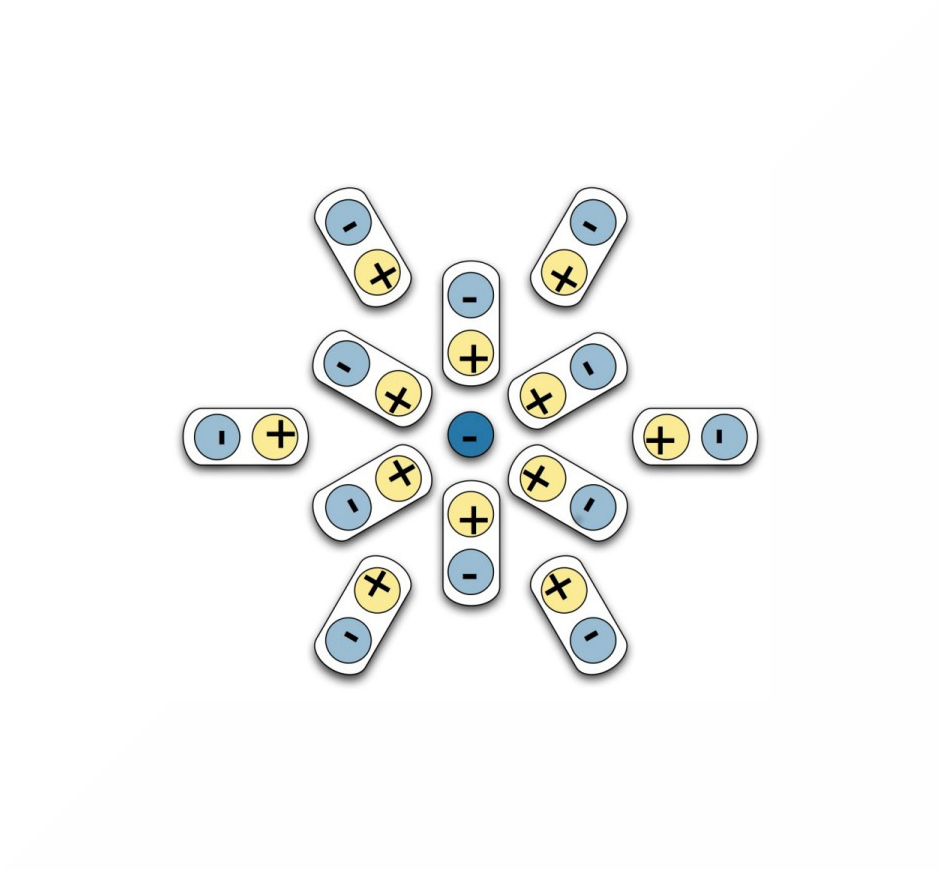
\includegraphics[scale=0.22]{figures/pol.jpg}\label{pol}}\quad
  \subfloat[][]
  {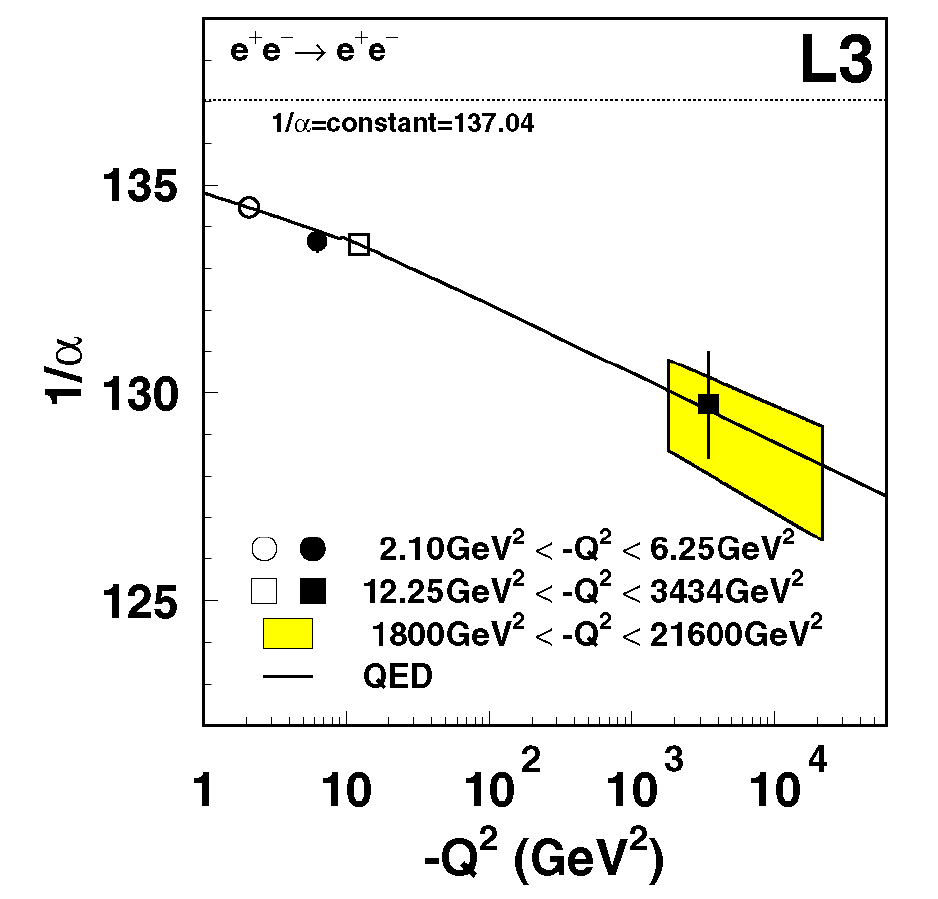
\includegraphics[scale=0.25]{figures/qedalpha.png}\label{qedalpha}}
  \caption{(a) Example of polarization (b) Measurement of the running of the electromagnetic coupling as a function of momentum-transfer at LEP \cite{achard2005}.}
\end{figure}
%
In QCD, instead, the coupling constant $\alpha_{S}$ has a different behaviour, due to the fact that there are gluon loops besides fermion loops. Indeed the renormalization theory shows that bosonic and fermionic loop contributions have opposite signs: besides the screening of the colour charge, like for electric charge in QED, there is an antiscreening effect due to gluon loops.\\
The evolution of the strong coupling constant is given by equation:
%
\begin{equation}
 \alpha_{S}(|Q|^{2})= \frac{ \alpha_{S}(\mu^{2})}{1+\frac{\alpha_{S}(\mu^{2})}{12\pi}(33-2n_{f})ln(|Q|^{2} / \mu^{2})}
 \label{eq:aqcd}
\end{equation}
%
where $n_{f}$ is the number of the quark flavours effectively contributing to the loops, namely those with mass $m_{f} < |Q|$.
%
\begin{figure}
  \centering
  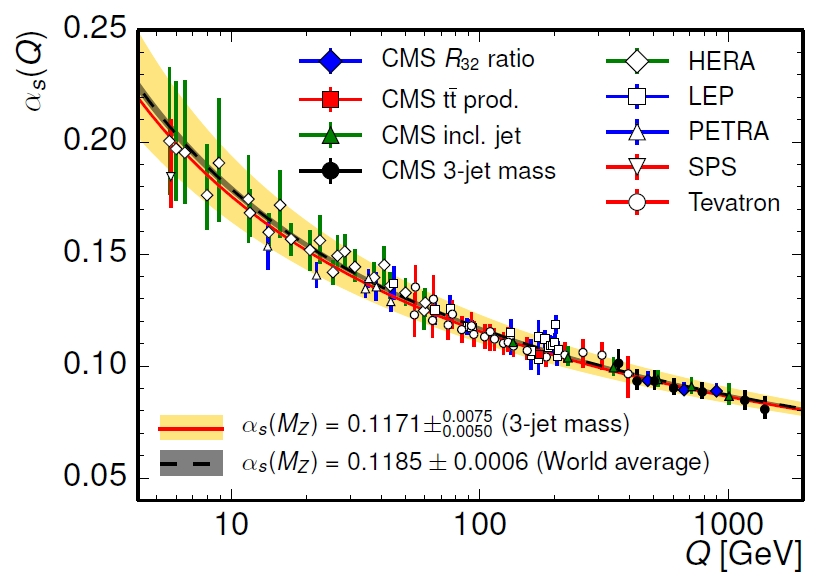
\includegraphics[scale=0.30]{figures/alphas_3j.jpg}
  \caption{Calculations and measurements of strong coupling constant $\alpha_{S}$ as a function of the energy scale Q \cite{kh2015}.}
  \label{fig:alphas}
\end{figure}
%
The value of $\alpha_{S}$ as a function of the energy scale Q can be seen in Figure \ref{fig:alphas}: it decreases when the transferred momentum increases, i.e. when the distance decreases. In particular, for small values of $Q^{2}$ the coupling constant assumes large values and the perturbative approach is not possible anymore.
For this reason, it is convenient to introduce the parameter $\Lambda_{QCD}$, which represents the limit energy scale for the perturbative approach. Using $\Lambda_{QCD}$ equation \ref{eq:aqcd} can be rewritten for large values of the transferred momentum ($|Q|^{2} \gg \Lambda^{2}$) as:
%
\begin{equation}
 \alpha_{S}(|Q|^{2})= \frac{12\pi}{(33-2n_{f})ln(|Q|^{2} / \Lambda^{2})}.
 \label{eq:aqcd2}
\end{equation}
%
For the above considerations, two regimes can be distinguished: asymptotic freedom and confinement.\\
Asymptotic freedom is the regime of high energy, where the coupling constant $\alpha_{S}$ is small enough to allow a perturbative approach: for $Q \sim$ 100 GeV - 1 TeV, $\alpha_{S}$ is about 0.1. For such energies the strong interaction becomes mild, reducing the energy necessary to divide colour charges and to release quark and gluons from their bound states. Since high $Q^{2}$ means short distances, it is possible to obtain this state of free partons by compressing or heating QCD matter: the result is a plasma of quark and gluons, the QGP, of which it will be discussed in the next section.\\
Confinement, instead, is the regime of low energy, where the perturbative approach is not valid anymore but other theoretical methods can be used, like, e.g., lattice QCD. In this range of energy, as already said before, the strong interaction becomes more important thanks to the formation of gluon loops and to the consequent antiscreening of the colour charges. Moreover, the energy necessary to separate two colour charges increases with the separation itself, making the system move towards a stable equilibrium characterized by the absence of free colour charges and by the formation of colourless states. Two methods used for the study of confined will be discussed in the next section.

\clearpage

\section{QCD phase space diagram}
%
\begin{figure}
  \centering
  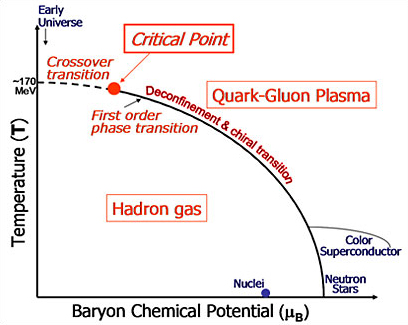
\includegraphics[scale=0.5]{figures/phase.jpg}
  \caption{Phase diagram for strongly interacting matter}
  \label{fig:phase}
\end{figure}
%
Nuclear matter is expected to exhibit different behaviours depending on its temperature T and baryo-chemical potential $\mu_{b}$. The latter is defined
as the energy needed to increase by one unity the total number of baryons and anti-baryons, $\mu_{B}= \partial E / \partial N_{B}$, and is related to the baryon density. An example of phase diagram is given in Figure \ref{fig:phase}.\\ At low temperatures and small $\mu_{B}$ ($\sim$1 GeV), nuclear matter is confined in hadrons and atomic nuclei. A state of hadronic gas can be reached either by increasing T or compressing the nuclear matter, i.e. increasing $\mu_{B}$: in these conditions, the nucleons can interact and form pions, excited states or other hadrons.
For even larger values of T and $\mu_{B}$ the transition to the phase of QGP, a state of deconfined strongly interacting matter, is predicted. These conditions necessary to the formation of QGP existed in the very first stages of the Universe: in facts, according to the Big Bang theory, about fourteen billion years ago the Universe was concentrated in a very small region of space, characterized by almost infinite temperature and energy, and then it started expanding and consequently cooling down. In the first stages, corresponding to few microseconds after the Big Bang, the temperature was so high that hadrons could not be formed and all the strongly interacting matter existed in form of QGP. However, for the expansion and the cooling, the energy density and the temperature of the Universe decreased under critical values, respectively $\epsilon_{c}\approx1 \;$GeV$/fm^{3}$ and $T_{c}\approx 170\; $MeV $ \approx 2\cdot10^{12}\; K$, for which a state of deconfined matter was not possible anymore, causing the transition to a confined state.\\ Unfortunately, it is not possible to observe the characteristics of this primordial state, since the transition from deconfined to confined matter took place when the electromagnetic radiation was still coupled with the primordial plasma constituting the universe, which therefore was opaque. For this reason, the only way to study the characteristics of the QGP, and of the transition from this to the hadronic phase, is to recreate these conditions using high energy heavy ions collisions, as it will be seen farther.
However, in orther to describe the evolution of QGP and, above all, the hadronization, it is not possible to use the perturbative approach for the reason said before and some methods to describe confined strongly interacting matter are needed.

\subsection{MIT bag model}

The MIT bag model is an effective model that describes, in a phenomenological way, quarks and gluons confined within the hadrons. Even if based on very simple hypothesis, the MIT bag model allows to give a description of confinement and phase transition, giving rough estimations of the critical temperature $T_{C}$, corresponding to the transition from deconfined to confined strong interacting matter. In the MIT bag model quarks are seen as massless fermions inside a spherical bag of finite dimensions, whose confinement is due to the balance between the pression exerted from the particles on the bag, coming from their kinetic energy, and an external pressure \textit{ad hoc} introduced, which takes into account effects that cannot be calculated through a perturbative approach. Considering these hypotheses, it is possible to evaluate the pressure on the bag for a confined state.\\
The equation of motion for a massless fermion is the Dirac equation:
%
\begin{equation}
  \gamma^{\mu}p_{\mu}\psi=0
\end{equation}
%
Imposing the confinement conditions means that on the surface of the bag the scalar density must be null:
%
\begin{equation}
  \overbar{\psi}\psi \Big|_{bag} = 0 \ \ \ \longrightarrow \ \ \ E = \frac{2.04 \hbar c}{R},
\end{equation}
%
where R is the radius of the bag.\\
Calling B the external pressure on the bag, the total energy of the system is equal to:
%
\begin{equation}
  E = \frac{2.04N \hbar c}{R} + \frac{4}{3} \pi R^{3} B,
\end{equation}
%
being N the number of particles within the bag.\\
From this equation, the radius of the bag and the external pressure B can be determined imposing the equilibrium condition, in other words minimizing the energy:
%
\begin{equation}
  \frac{dE}{dR} = -\frac{2.04 \hbar c}{R^{2}} + 4 \pi R^{2} B = 0 \ \ \ \longrightarrow \ \ \ B^{\frac{1}{4}} = \frac{\hbar c}{R}\Big(\frac{2.04N}{4\pi}\Big)^{\frac{1}{4}}
\end{equation}
%
Considering a baryon composed of three valence quarks, with a radius of 0.8 fm, the value of the fourth root of the external pressure is $B^{\frac{1}{4}} = 206 \; $MeV$ / (\hbar c)^{3/4}$. In this way, the effects of non perturbative QCD are included in the external pressure B, expressly introduced for this reason, and this pressure is balanced from the internal pressure exerted by the quarks. According to the MIT bag model, the phase transition can be seen as the increase of the internal pressure to the point at which it overcomes the external one, giving birth to a new phase in which quarks are no more confined within hadrons, but free to move in a bigger volume: the state of QGP is therefore enhanced.\\
The internal pressure can increase in two ways: by compression, i.e. increasing the baryonic density, or by increasing the temperature, i.e the kinetic energy of the quarks. Focusing on the latter, it is possible to obtain the temperature at which the phase transition occurs, requiring the external pressure to match the internal one: 
%
\begin{equation}
  P = 37 \frac{\pi^{2}}{90}T^{4}_{C} = B \ \ \ \longrightarrow \ \ \ T_{C} = \Big(\frac{90B}{37\pi^{2}}\Big)^{\frac{1}{4}}= 145 \ MeV
\end{equation}
%
As far as concerns the MIT bag model, a transition from nuclear matter to QGP is expected at $T_{C} = 145$ MeV. However, as already said, this result comes from simple hypotheses and, for this reason, a more precise result can be obtained using more sophisticated methods, such as lattice QCD, which will be discussed in the next section.\\

\subsection{Lattice QCD}
%
Lattice QCD is the main tool to study non-perturbative aspects of QCD and is based on the discretization of the space-time, treated, indeed, as a lattice. This theory offers important advantages: first of all, if in the perturbative approach there is the problem of the divergence of the integrals with respect to the momentum for large values of this, which can be solved using a renormalization method, in lattice QCD this problem does not exist because the pitch of the lattice defines a minimum distance and consequently a cut-off value for the momentum. Then, the lattice partition function can be written as a path integral and, therefore, easily calculated, for example using Monte Carlo methods. On the other hand, the computational cost of numerical simulations can increase dramatically as the lattice spacing decreases, causing a constrain on the minimum pitch to use for the calculations. Moreover, in order to reduce the computational burden, further approximation are needed. For example, one of the most common approximation is the so called \textit{pure gauge}, in which quarks are considered as static sources of the colour field, fixed in the knots of the lattice, that is equivalent to considering the masses of the quarks infinite. Corrections to include the finite masses of the quarks and a not-null baryo-chemical potential are possible but under development.\\
In order to explain the basics of lattice QCD, the quantum mechanics case will be first considered for simplicity; then, it will be extended to quantum field theory.
The grand canonical partition function of the system at a temperature T can be written as:
%
\begin{equation}
 Z = \sum\limits_{x_{a}}\langle x_{a} | e^{-\beta T} | x_{a} \rangle
\end{equation}
%
where the sum is over all the possible states $x_{a}$ of the system, $\beta=1/T$, and H is the hamiltonian operator.\\
This formula is very close to Feynman path integrals:
%
\begin{equation}
 \langle x_{b} | e^{- i H (t_{b} - t_{a})} | x_{a} \rangle = \int \prod\limits_{i=1}^{n_{t}-1} dx_{i} e^{i S_{M}(x_{a},x_{1},\dots,x_{n_{t}-1},x_{b})}
\end{equation}
where $x_{a}$ and $x_{b}$ are initial and final position, respectively at time $t_{a}$ and  $t_{b}$, $x_{i}$ is any of the $n$ intermediate positions in which it has been decided to divide the path and $S_{M}$ is the minkowskian action.\\
The two previous expressions are very alike, but there are few differences and, for this reason, in order to express the partition function as a path integral, some precautions are needed. First of all, the exponent of the former is real, while the one of the latter is imaginary: it can be solved using a change of variable $t = -i \tau$, known as \textit{Wick rotation}, that is equivalent to using an imaginary time and passing from a minkowskian to an euclidean action. Then, in the partition function formula, initial and final states are the same: this problem can be solved imposing periodic boundary conditions, i.e. $x(\tau_{b}) = x(\tau_{b})$. Choosing appropriate $\tau$ boundaries, i.e. $\tau_{a} = 0 \leq \tau \leq \tau_{b} = \tau_{n_{t}}$, the previous condition can be written as $x_{a} = x(\tau_{n_{t}})$ and the expression for Z becomes:
%
\begin{equation}
 Z = \int dx_{n_{t}} \prod\limits_{i=1}^{n_{t}-1}dx_{i} \; e^{iS_{M}\Big|_{t=-i\tau}} = \int \prod\limits_{i=1}^{n_{t}}dx_{i} \; e^{-S_{E}} \equiv \int \mathcal{D}x \; e^{-S_{E}(x)}
\end{equation}
%
The last step is the extension to the quantum field theory:
%
\begin{equation}
 Z = \int \mathcal{D}\phi(x,\tau) \; e^{-S_{E}(\phi(x,\tau))}
\end{equation}
%
The most efficient numerical approach to calculate path integrals is to estimate thermal averages over specific paths, which are identified using Monte Carlo algorithms of importance sampling. Then, the path integrals are evaluated introducing a four-dimensional space-time lattice, whose spacing is the smallest permitted by the computational limits.\\
As already said before, using lattice QCD it is possible to get more precise prediction about the phase transition, but its characteristics are, for example, strongly dependent on the treatment of quark masses and precise calculations are available only in the limit of vanishing baryo-chemical potential ($\mu_{B}\sim0$). In particular, in the limit of two quarks flavours with null mass, a second-order transition is predicted, while a first-order one is foreseen in case of three massless quarks. However, recent calculations of lattice QCD predict a critical an estimated temperature $T_{C}\approx160$ MeV, corresponding to an energy density $\epsilon_{C} = 0.7 \pm 0.3$ GeV$/fm^{3}$\cite{lattice}.

\section{Heavy ions collisions}
In order to study the properties of the QGP, it is necessary to create a system of strongly interacting matter at extreme conditions of temperature and energy density, which could be described using the thermodynamics. For this reason, this system should be characterized by a wide spatial extension, so that it could be described using macroscopic variables, such as the temperature or the pressure. Therefore, first, the system must have an extension which must be much greater than the strong interaction scale ($\sim$ 1 fm); then, it must be characterized by a great number of particles (high multiplicity). Furthermore, the system must be long lived, so that a high number of collisions between the constituents can occur and lead to thermal equilibrium, necessary for using a thermodynamic approach. The thermal equilibrium is reached when the free mean path of the constituents ($\tau_{path}$) is greater than the system dimension and smaller than the life time of the system ($\tau_{system}\gg\tau_{path}$). These hypothesis has to be verified comparing the theoretical prediction with the experimental data. However, in high energy nucleus-nucleus collisions, all these requirements are expected to be fulfilled, thanks to the multiple collisions between nucleons of the colliding nuclei. In facts, a nucleon collides with many nucleons in the other nucleus, releasing energy. For this reason, there is a large energy deposit in the interaction region, determining a high energy density of the system and, therefore, a high temperature. Moreover, a large number of primary particles is produced, determining the high multiplicity required as hypothesis.\\
In the next sections, it will be shown how to describe nucleus-nucleus collisions and how this kind of events evolves.\\

\subsection{Glauber Model}
The Glauber Model provides a description of the nucleus-nucleus interaction as an incoherent superposition of nucleon-nucleon collisions.
The key element of the Glauber model is the impact parameter $\vec{b}$, a geometrical parameter defined as the distance between the centres of the two nuclei in the transverse plane. The impact parameter is important because it determines the centrality of the collision. Central collisions are characterized by a small impact parameter: in this kind of events many nucleons are involved in the interaction and, therefore, there are many collisions between nucleons and many particles are produced. Peripheral collisions, instead, are characterized by a large impact parameter: the overlap region is smaller and so there are few nucleons involved in the interaction, hence few collisions between nucleons and few particles produced.\\
The Glauber Model is based on few assumptions, also known as \textit{optical limit}:
\begin{itemize}
 \item the nucleons are point like;
 \item the nucleons inside the nuclei are independent;
 \item the nuclei, hence the constituent nucleons, travel in a straight line: there are no deflections;
 \item only the strong interaction is considered: protons and neutrons cannot be distinguished;
 \item the cross section for an elementary nucleon-nucleon interaction is the same for all the passage of the nucleon through the target.
\end{itemize}
During the collisions we can distinguish two kinds of nucleons: the spectators are those nucleons that do not interact with any nucleon of the other nucleus; the participants are the nucleons which have interacted at least with a nucleon of the other nucleus.\\
Even if this model is based on simple hypotheses, it allows to get much information, such as the probability of interaction, the number of elementary collisions, the number of participant nucleons, the number of spectators, etc.
%
\begin{figure}
  \centering
  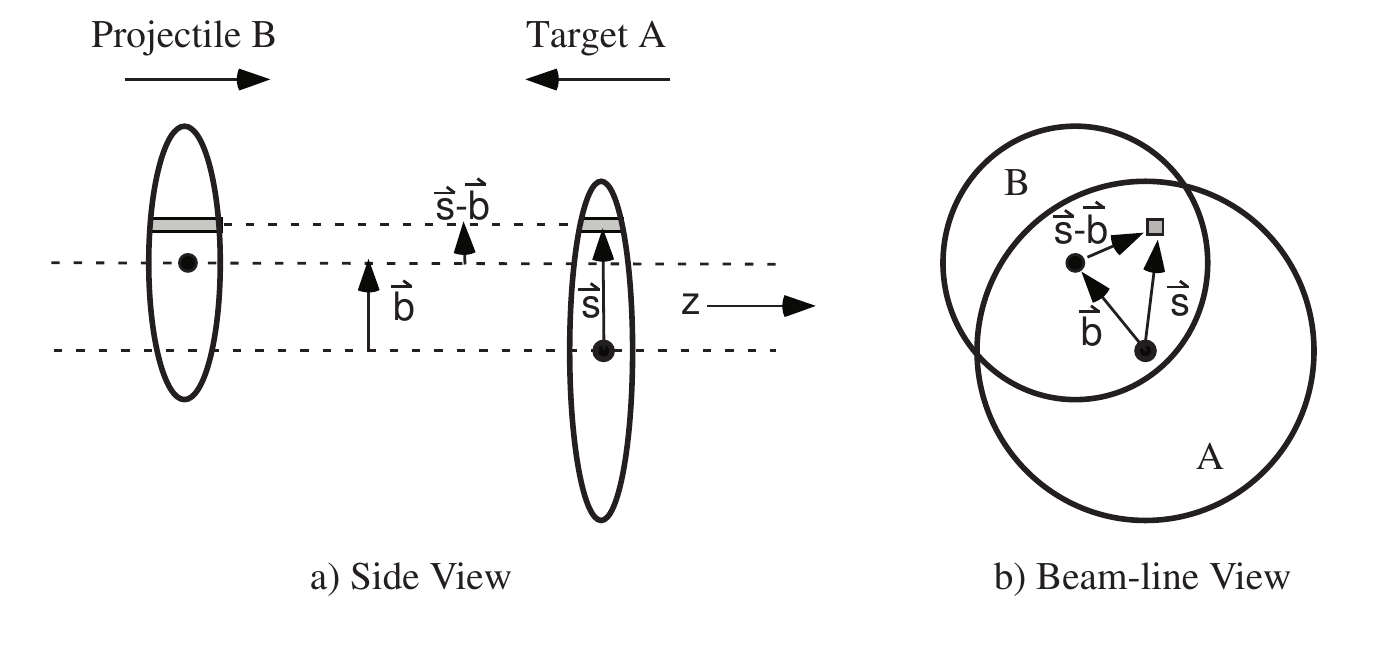
\includegraphics[scale=0.30]{figures/Impact_parameter.png}
  \caption{Schematic view of a nucleus-nucleus collision in the longitudinal (a) and transverse (b) plane.}
  \label{fig:impact}
\end{figure}
%
\subsection{Rapidity and Pseudorapidity}
Before describing the evolution of a nucleus-nucleus collision, it is necessary to introduce two important variables, essential for the description of these phenomena: the rapidity \textit{y} and the pseudorapidity $\eta$.\\
The rapidity is the parameter that arises in the linear representation of a Lorentz boost:
\begin{equation}
 \left(
    \begin{array}{c}
      E'\\
      p'_{\:\parallelsum}
    \end{array}
  \right) = 
      \begin{pmatrix}
      \cosh y & \sinh y \\
      \sinh y & \cosh y 
    \end{pmatrix}
  \;
  \left(
     \begin{array}{c}
      E\\
      p_{\:\parallelsum}
    \end{array}
  \right)
\end{equation}
%
From this equation, it can be easily shown that the rapidity, assuming a Lorentz boost along z direction, which is the beam direction, can be expressed as:
\begin{equation}
 y = \frac{1}{2}\ln\frac{E + p_{z}}{E - p_{z}}
\end{equation}
However, from an experimental point of view, the determination of the rapidity requires the identification of the particle, which, in certain cases, could be very difficult, or the measurement of two different quantities, such as $E$ and $p_{z}$. Therefore, this variable is often substituted by the pseudorapidity $\eta$, which is related uniquely to the polar angle $\theta$ by the expression:
\begin{equation}
 \eta = \frac{1}{2}\ln\frac{|\vec{p}\:| + p_{z}}{|\vec{p}\:| - p_{z}} = - \ln [\tan (\theta/2)]
\end{equation}
In the high energy limit, it can be shown that $\lim_{\beta \to c} \eta \;= \;y$.\\
These two parameters are extremely important, since many variables, like, for example, the multiplicity, are described in terms of rapidity or pseudorapidity.\\


\section{Evolution of nucleus-nucleus collisions}
The collision between two ultra-relativistic nuclei is an event characterized by a complex space-time evolution: a scheme of this process can be found in Figure \ref{fig:evol}.\\
Before the collision takes place, the two nuclei travel along the beam direction at a speed close to the speed of light and, for this reason, they are Lorentz-contracted. This means that the two nuclei can be represented as two disks.\\
At $t=0$, the two nuclei collide, hence scatterings between the nucleons of the projectile and of the target take place. In each of this collision, the nucleons lose energy ad momentum and, in case of inelastic scattering, they could become unstable baryon-like objects. Withal, at the LHC energies, after the interactions these products still have enough energy to escape the interaction region, which, in the case of a symmetric collider such as the LHC, is the mid rapidity region ($y\sim0$), and decay far away from this region. Therefore, for high energy collisions, the mid-rapidity region is characterized by a high energy density, with the generation of $q\bar{q}$ pairs, but with a low baryonic content, i.e. a vanishing baryo-chemical potential ($\mu_{B}\sim$ 0). All together these conditions form the so called \textit{transparency regime}. The transparency regime is characterized by a large number of particle for unity of rapidity ($\frac{dN}{dy}$) in the mid rapidity region. Therefore, in these distributions a plateau around $y\sim0$, whose width and height is determined by the energy of the collision, is expected.\\
If the temperature of the medium created is larger than a critical value $T_{C}$, the formation of a system of deconfined quarks and gluons is expected. The QGP could be initially not in thermal equilibrium but, thanks to the high number of scatterings, it should thermalize at a proper time $\tau_{0}$, whose value strongly depends on the centre of mass energy of the experiment. At the LHC energies, for example, $\tau_{0}<$ 0.2 fm/c. After $\tau_{0}$, the system is expected to evolve according to the hydrodynamics: the plasma expands and for this reason the temperature decreases until it reaches the critical value $T_{C}$ and the process of hadronization starts. In case of first order transition, the system is characterized by a mixed phase, where the QGP coexists along with confined hadronic matter. This mixed phase lasts for a time $\tau\sim$ 10 fm/c, after which the system appears as a gas of hadrons, in which a large number of scatterings, both elastic and inelastic, can take place.
When the temperature reaches values for which the inelastic scatterings are not possible anymore, the chemical composition is fixed: this moment is called chemical freeze-out and occurs at a temperature $T_{ch}$. After the chemical freeze-out, the system continue expanding and the elements interact via elastic scatterings until the temperature drops below the vale $T_{kin}$, at which the thermal freeze-out occurs. After the thermal freeze-out, the hadrons finally stream out of the collision region. Typical values of the chemical and thermal freeze-out temperatures, estimated at the LHC in central Pb-Pb collisions at $\sqrt{s_{NN}} =$ 2.76 TeV, are $T_{ch}\sim$ 160 MeV and $T_{kin}\sim$ 100 MeV \cite{temp}.
%
\begin{figure}
  \centering
  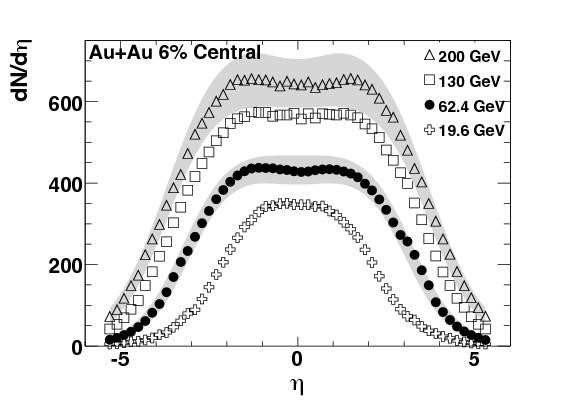
\includegraphics[scale=0.5]{figures/dNdeta.png}
  \caption{Charged particle multiplicity distributions for collisions at RHIC with four different energies as a function of pseudorapidity\cite{dndeta}.}
  \label{fig:dndeta}
\end{figure}
%
%
\begin{figure}
  \centering
  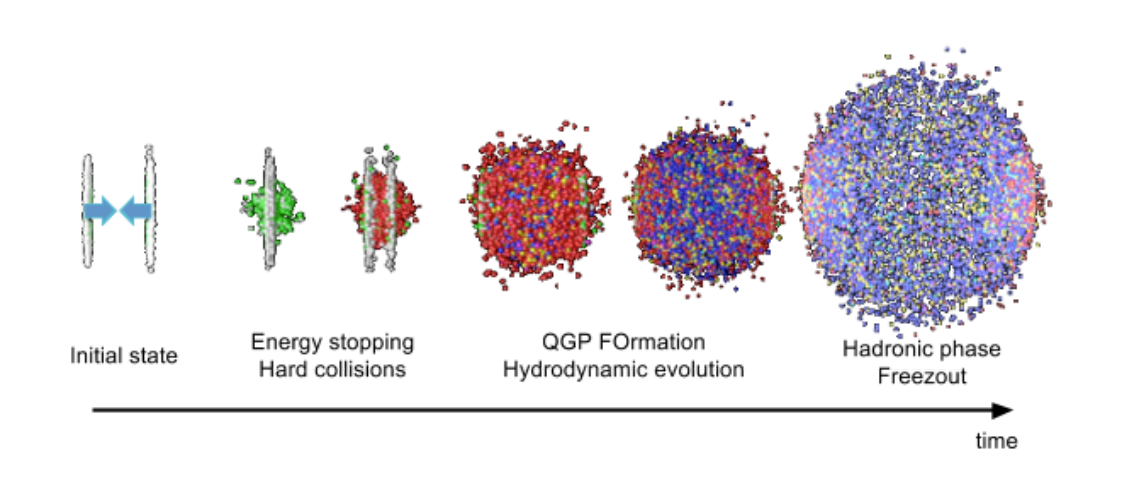
\includegraphics[scale=0.5]{figures/evolution.png}
  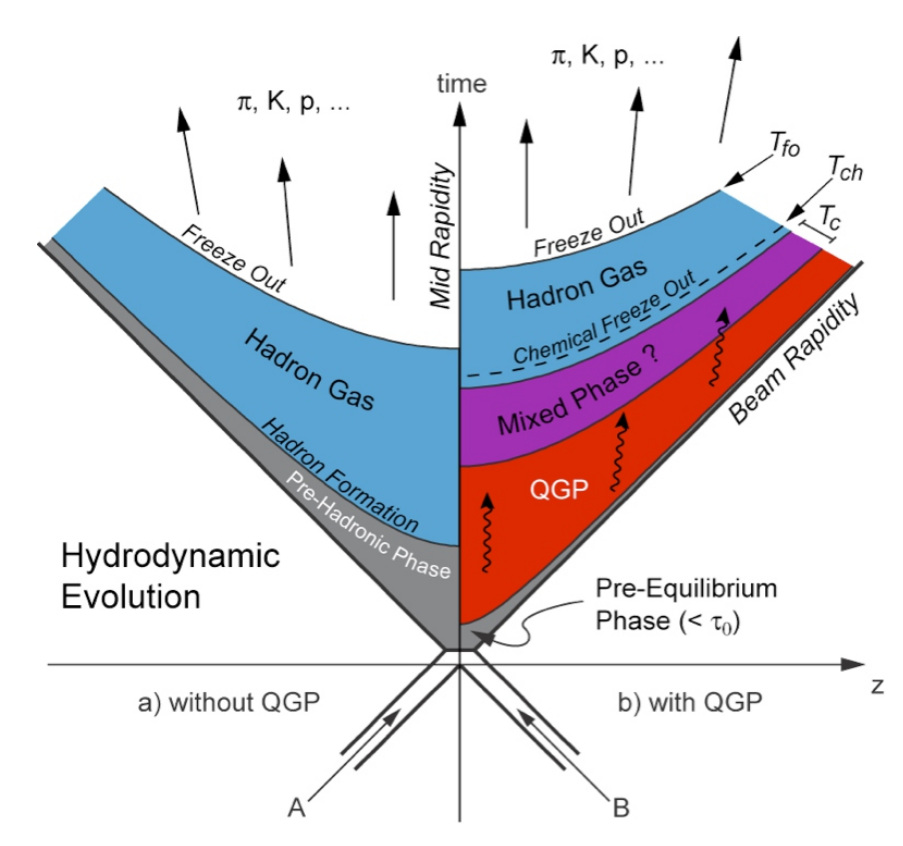
\includegraphics[scale=0.35]{figures/spacetime.png}
  \caption{Space-time evolution of a collision between nuclei, described with a hydrodynamic approach.}
  \label{fig:evol}
\end{figure}
%
\clearpage
\section{Experimental observables in ALICE}
Since the QGP, from an experimental point of view, is characterized by a short life time (few $10^{-23}$ s), the direct measurement of variables such as, for example, temperature, is not possible. Indeed, the only accessible variables are those that characterize the final state, i.e. those related to the particles present in the last stage of the collision process, as previously described. For this reason, the theoretical models are extremely important to define which characteristics of the final state could provide information about the QGP formation and the phase transition. In facts, comparing the experimental measurements with the theoretical predictions, it is possible to indirectly determine important quantities, which are parameters of the theoretical models, related to stages of the evolution of the system otherwise not accessible.\\
These quantities can be measured considering different kinds of probes: electroweak probes and hadronic probes. The formers (dielectrons and direct photons) are related to the early stages of the evolution of the fireball. In facts, they do not interact strongly and so they can pass through the generated medium unharmed. However, they are less abundant then the hadronic probes and, concerning the direct photons, it is difficult to divide these from the background generated in the following stages. The hadronic probes, otherwise, are more abundant but are influenced by the medium and by the final state effects. Consequently, it is difficult to distinguish particles produced in the earliest stages of the collision from those generated in later stages or in hadronic processes.\\
It is also possible to make another distinction among the probes, according to the value of the transferred momentum of the process in which they have been generated.\\
The hard probes are produced in the first stages of the collision, when the energy of the system has not degraded yet, in processes characterized by a high momentum transfer, like, for example, the interaction between high momentum partons. They are rare processes, whose number scales with the number of collisions among the nucleons constituting the projectile and the target nuclei, and are sensible to the following stages of the collision. The soft probes, instead, are produced in the last stages of the collisions, by processes characterized by a low momentum transfer. For this reason, they cannot resolute the the partonic structure of the nucleons. However, even if they are produced during the hadronic stage, they keep indirect information on the properties of the phase transition and on the QGP. Then, the soft probes constitute the bulk of the hadrons produced in the collision, above the 99$\%$.\\
In the next sections, the most important observables for ALICE will be described.\\
\subsection{Particle multiplicity}
The multiplicity is the number of particles produced in a collision. Two kinds of multiplicity measurements can be distinguished: the multiplicity of not identified particles, i.e. the total number of particles produced, and the multiplicity of identified particles, i.e. the number of particles of a certain species.
\subsubsection{Multiplicity of not identified particles}
In the study of the collisions between nuclei, this quantity is extremely important, since it gives information about the centrality of the collision, the energy density of the final state and the mechanisms of particles production. Moreover, it is also an important parameter for the design of an experiment for the study of ions collisions, since the occupancy of the detectors is closely related to the density of particles, hence to the multiplicity. Similarly, the radiation damage is related to the flow of the particles through the detectors and the readout electronics. As far as concerns the ALICE experiment, this was designed to run with multiplicity up to 8000 particles per unit of rapidity in the mid-rapidity region. However, this estimation was made in a period when RHIC multiplicity data were not available and happened to be overestimated, since the measured value is approximately 1600 charged particles per rapidity unity\cite{mult}.\\  
As mentioned before, the multiplicity is related to the centrality of the collision, i.e. to the value of the impact parameter. In facts, for the Glauber Model, both the number of elementary collisions and the number of participant nucleons are related to the impact parameter. Since in each elementary collision there is a release of energy, each collision contributes to the production of particles, then to the multiplicity. Typically, the measure of the total cross section per charged particle as a function of the charged multiplicity is used to express the centrality, as shown in Figure \ref{fig:centr}: it is expressed as the percentage of area under curve.\\
%
\begin{figure}
  \centering
  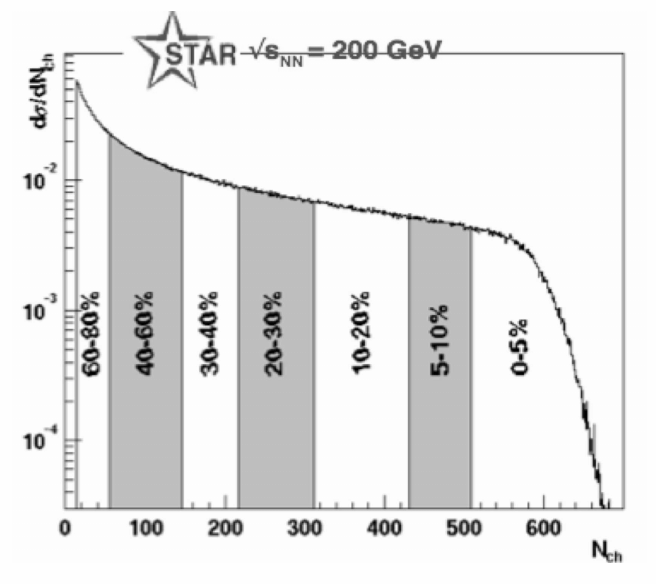
\includegraphics[scale=0.5]{figures/star.png}
  \caption{A typical event multiplicity distribution at RHIC, sliced up in centrality classes.}
  \label{fig:centr}
\end{figure}
%
Then, the measurement of the charged multiplicity per pseudorapidity unity at mid-rapidity allows an estimation of the energy density of the QGP, using a method proposed by Bjorken.\\
According to this method, in the frame in which both the colliding nuclei have high energy, the projectile and the target, that are Lorentz contracted, can be seen as two disks that rapidly pass through each other. Then, secondary particles are generated in this region bounded by the two disks, which is characterized by a low longitudinal extension. A scheme of this model can be seen in Figure \ref{fig:bjor}.\\
%
\begin{figure}
  \centering
  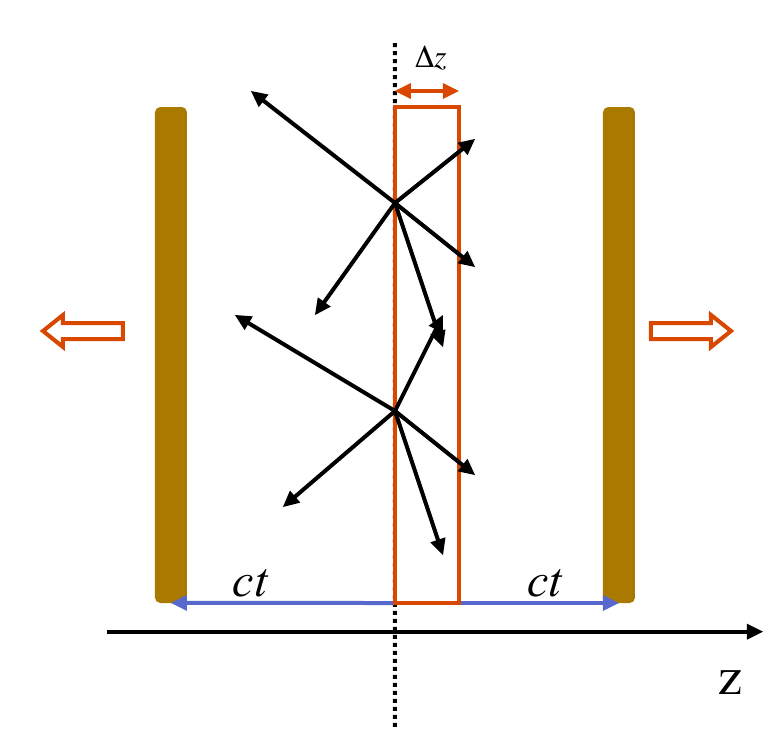
\includegraphics[scale=0.3]{figures/bjorken.png}
  \caption{A scheme of Bjorken's model for the collision between high energy nuclei.}
  \label{fig:bjor}
\end{figure}
%
According to these hypotheses, the mid-rapidity region is characterized by a certain number of particles that have formed at a time $\tau_{0}$. It is possible to determine the energy density of this region at the time of formation of these secondary particles, considering the region of longitudinal width $\Delta z$ and transverse section \textit{A} shown in Figure \ref{fig:bjor}. This region includes all the particles with a longitudinal speed in the range 0 $\leq \beta_{z} \leq \frac{\Delta z}{\tau_{0}}$. Therefore, the number of particles within this region is given by the expression:
\begin{equation}
 \Delta N \;=\; \int_{0}^{\frac{\Delta z}{\tau_{0}}} \frac{dN}{d\beta_{z}}d\beta_{z}\;\cong\;\frac{\Delta z}{\tau_{0}}\frac{dN}{d\beta_{z}}\;=\;\frac{\Delta z}{\tau_{0}}\frac{dN}{dy},
\end{equation}
where in the last passage the approximation $\beta_{z}\sim y$ has been done, since the rapidity is almost null. Then, since the rapidity is close to zero, the energy of the particles coincides with their transverse mass $m_{T} = \sqrt{m_{0}^{2} + p_{T}^{2}}$, since $E = m_{T} \cosh y \cong  m_{T}$. Hence, the average energy density of this region is:
\begin{equation}
 \langle \epsilon(\tau_{0}) \rangle \; = \; \frac{\Delta N\langle m_{T}\rangle}{\Delta z\:A}\;=\;\frac{\Delta z}{\tau_{0}}\frac{dN}{dy}\frac{\langle m_{T}\rangle}{\Delta z\:A}\;=\;\frac{1}{\tau_{0} A} \langle m_{T} \rangle \frac{dN(\tau_{0})}{dy}\;=\;\frac{1}{\tau_{0} A}\frac{dE_{T}(\tau_{0})}{dy},
\end{equation}
where $E_{T}$ is the transverse energy and \textit{A} is the area of the overlapping region.\\
Summing up, at mid-rapidity the energy density can be determined using the Bjorken's formula:
\begin{equation}
 \epsilon_{Bj}\;=\; \frac{1}{\tau_{0} A}\frac{dE_{T}}{dy}\Big|_{y=0}\;\sim\;\frac{1}{\tau_{0} A}\langle E_{T} \rangle \frac{dN}{d\eta}\Big|_{\eta=0}
\end{equation}
Measuring the pseudorapidity density $\frac{dN}{d\eta}$ and the average hadron energy transverse energy $\langle E_{T} \rangle$, which can be obtained experimentally by measuring the energy of charged hadrons, if an estimation of the time of formation $\tau_{0}$ is given, the energy density can be easily determined. ALICE obtained for Pb-Pb collisions in the centrality range 0-5 \% $\epsilon_{Bj} \approx$ 16 GeV/fm$^{3}$, considering a formation time $\tau_{0}$ = 1 fm/c. The energy density is so well above the critical energy density $\epsilon_{C} \sim$ 1 GeV/fm$^{3}$ expected for the phase transition according to the lattice QCD calculations.\\
Finally, it is interesting to compare the charged multiplicity, normalized using the number of participants nucleons, in ions collisions with the value obtained in p-p collisions. The normalization factor is important for this comparison, since in p-p collisions there are always two participants, while in ion collisions the number of participants depends on the centrality of the event and, for this reason, it is important to fix the centrality range.
%
\begin{figure}
  \centering
  \subfloat[][]
  {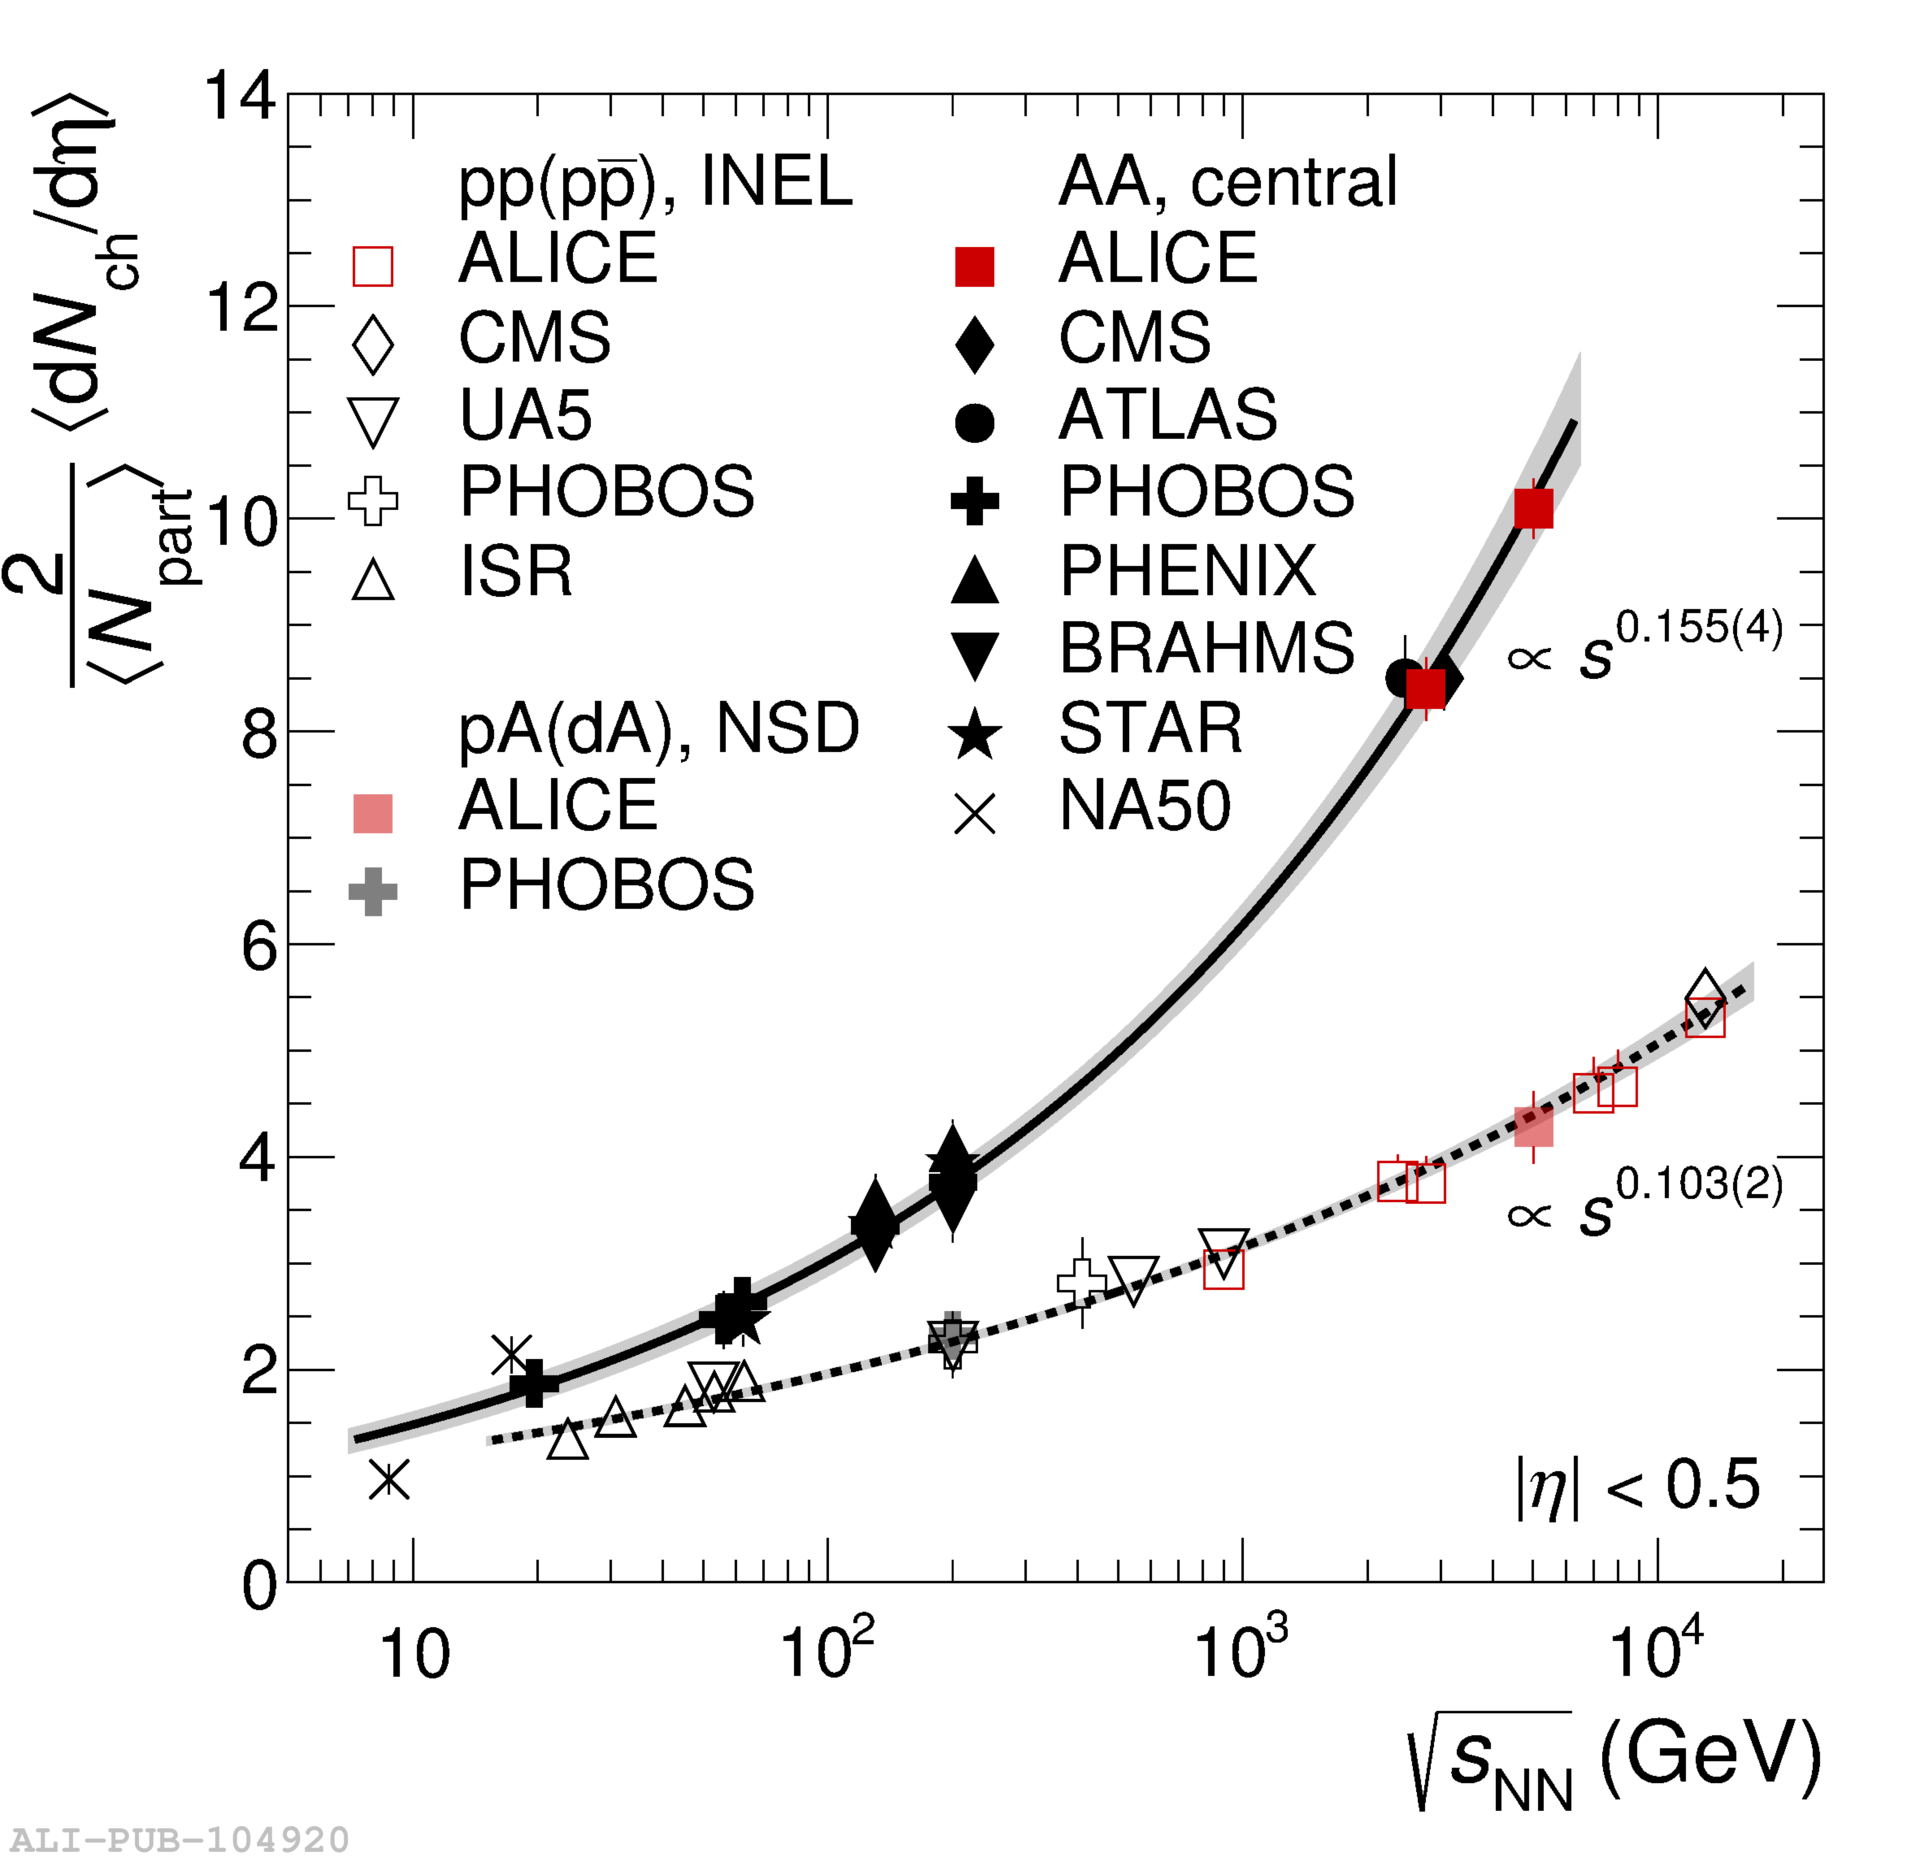
\includegraphics[scale=0.3]{figures/multen.png}\label{fig:multen}}\quad
  \subfloat[][]
  {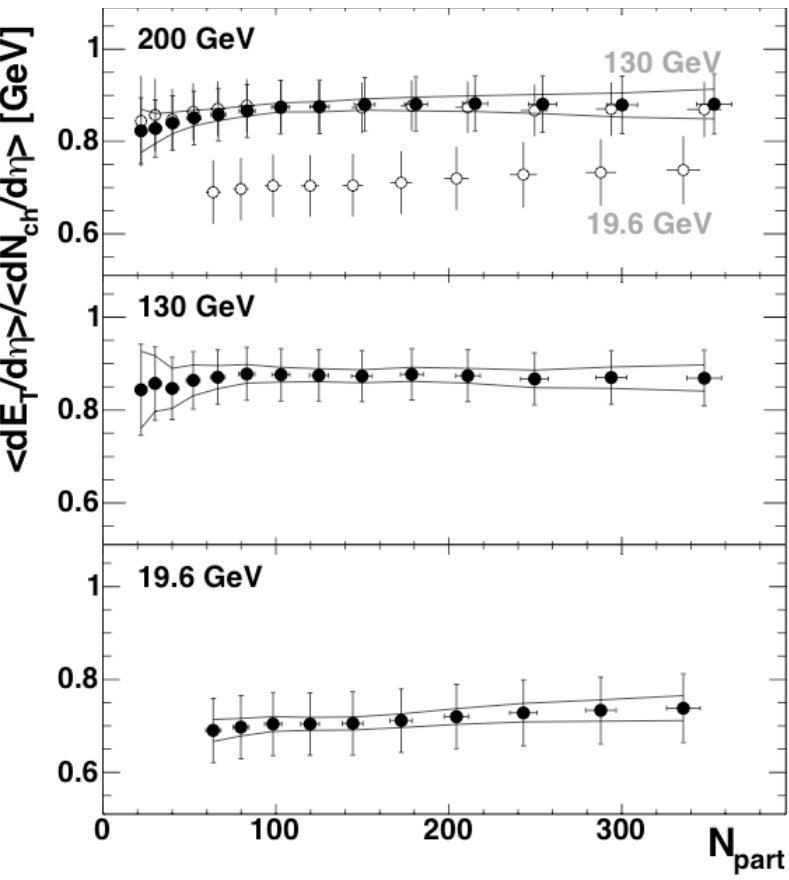
\includegraphics[scale=0.35]{figures/phenix.png}\label{fig:phenix}}
  \caption{(a) Charged pseudorapidity density per participant pair for nucleus-nucleus and p-p collisions, as a function of $\sqrt{s_{NN}}$ \cite{multen}. (b) Ratio between pseudorapidity energy density and pseudorapidity density as a function of the number participants for different values of $\sqrt{s_{NN}}$ at PHENIX experiment.}
\end{figure}
%
In Figure \ref{fig:multen}, the pseudorapidity per participant pair is shown as a function of the energy $\sqrt{s_{NN}}$: the particle production trend is steeper in AA than what obtained in p-p collisions.\\
Then, considering the ratio between the energy pseudorapidity density $\frac{dE}{d\eta}$ and  the pseudorapidity density $\frac{dN}{d\eta}$ as a function of the number of participants, it can be seen that this quantity does not change much with $\sqrt{s_{NN}}$. This means that the extra energy goes into the production of new particles rather than into kinetic energy.\\
\subsubsection{Multiplicity of identified particles}
The measurement of the multiplicity of the hadronic species. i.e. of the chemical composition of the system after the hadronization, allows to get important information about the state of the system at the chemical freeze-out, like, for example, whether the fireball was at the equilibrium or not, the temperature and the baryonic content.\\
The abundances of the different hadronic species produced in an ion collision can be described using the so called \textit{statistical thermal model}, which is based on the hypothesis that the system is at chemical and thermal equilibrium when the chemical freeze-out occurs. With this assumption, it is possible to describe the system using the statistical mechanics, in particular using a grand canonical ensemble with two parameters, the temperature and the baryo-chemical potential. It is important to note that the equilibrium is postulated: this model does not describe the evolution of the collision till the phase transition and not even how this transition takes place. It is a merely statistical equilibrium, due to the way in which the hadronization fills the phase space, realizing the most probable configuration. Secondly, the system is described as an ideal gas of hadrons and resonances (\textit{Hagedorn's gas}, from the name of the scientist who has developed the model). It contains all the degrees of freedom of a strongly interacting confined system, for not too high temperatures (T < 190 MeV). With this method, a gas of interacting hadrons is approximated by a gas of non interacting hadrons and resonances.\\
Using the grand canonical ensemble, the partition function for the gas just described is given by the product of the partition functions of each species:
\begin{equation}
 Z^{GC}(T,V,\mu)\; = \;\prod_{i}Z^{GC}_{i}(T,V,\mu_{i}),
\end{equation}
where, for the left hand side, the chemical potential $\mu$ is the parameter that in the grand canonical ensemble guarantees the average conservation of the quantum numbers:
\begin{equation}
\mu \; = \;\sum_{i} \mu_{Q_{i}}Q_{i},
\end{equation}
where $Q_{i}$ are the conserved quantum numbers, $\mu_{Q_{i}}$ are the chemical potentials associated to these quantities, and $\mu$ is the energy necessary to add to the system a particle with quantum numbers $Q_{i}$.\\
In the case of a gas of particles with a low mass (m < 1.8 GeV), i.e. without heavy quarks, there are three conserved quantum numbers: the third component of the isospin $I_{3}$, the baryonic number \textit{B}, the strangeness \textit{S}. Therefore, for each species $\mu_{i} = \mu_{I_{3}}I_{3i} + \mu_{B}B_{i} + \mu_{S}S_{i}$.
From the definition of the partition function for the single species:
\begin{equation}
 \ln Z_{i}\; = \; \frac{Vg_{i}}{2\pi^{2}}\int_{0}^{\infty}\pm\:p^{2}dp\ln[1\pm e^{-\frac{E-\mu_{i}}{T}}],
\end{equation}
the expression for the density can be derived:
\begin{equation}
n_{i}\; = \; -\frac{T}{V} \frac{\partial \ln Z_{i}}{\partial \mu} \;=\; \frac{g_{i}}{2\pi^{2}} \int_{0}^{\infty}\frac{p^{2}dp}{e^{-\frac{E-\mu_{i}}{T}}\pm1}.
\end{equation}
Finally, from this equation the average multiplicity of a particular species $\langle N_{i} \rangle$ can be easily defined.\\
Thanks to the knowledge of the electric charge, the strangeness and the baryonic number of the initial stage, only three parameters are necessary to estimate the average multiplicity: the temperature, the volume and the baryo-chemical potential. Moreover, if ratios between the multiplicity of different species are used instead of the multiplicity itself, the volume of the system, which is affected by a big uncertainty, is no needed.\\
In conclusion, the temperature and the baryo-chemical potential at the freeze-out can be determined through a $\chi^{2}$ minimization, using:
\begin{equation}
 \chi^{2}\;=\;\sum_{i}\frac{(R_{i}^{exp}-R_{i}^{model})^{2}}{\sigma_{i}^{2}}
\end{equation}
where $R_{i}$ are the ratios just described and $\sigma$ is the error associated to the measurements.\\
Considering the phase diagram, at the LHC the chemical freeze-out is extremely close to the phase transition predicted from the lattice QCD.\\
%
\subsection{Particle momentum spectra and radial flow}
The transverse momentum distributions (or transverse mass distributions) of the particles give an important information about the system created in the heavy ion collision, such as, for example, an estimation of the temperature of the thermal freeze-out. For these reason, there is the necessity to focus on the soft probes, those low transverse momentum particles generated in the last stages of the collision, which constitutes the bulk ($\sim$ 99\%) of the particle yield.\\
From the measurements in p-p collisions, it is known that the transverse mass distributions, normalized to the transverse mass, have an exponential trend:
\begin{equation}
 \frac{1}{m_{T}}\frac{dN}{dm_{T}}\; \propto \; e^{-\frac{m_{T}}{T_{slope}}} \ \ \ \longrightarrow \ \ \ \frac{dN}{dm_{T}}\; \propto \;m_{T}\: e^{-\frac{m_{T}}{T_{slope}}},
\end{equation}
where $T_{slope}$ has the same value for all the particles ($T_{slope} \approx $ 167 MeV).
Experimentally it is easier to measure the transverse momentum instead f the transverse mass, since the latter requires the identification of the particle, but the two distribution are equivalent, due to the easy change of variable:
\begin{equation}
 m_{T}\;=\;\sqrt{m^{2}+p_{T}^2} \ \ \ \longrightarrow \ \ \  p_{T}dp_{T}\;=\;m_{T}dm_{T}.
\end{equation}
Assuming that the observed distributions are thermal Boltzmann distributions, $T_{slope}$ is the temperature at which there is the emission of the particles, i.e. the thermal freeze-out. Hence, $T_{slope} \equiv T_{fo}$\\
%
\begin{figure}
  \centering
  \subfloat[][]
  {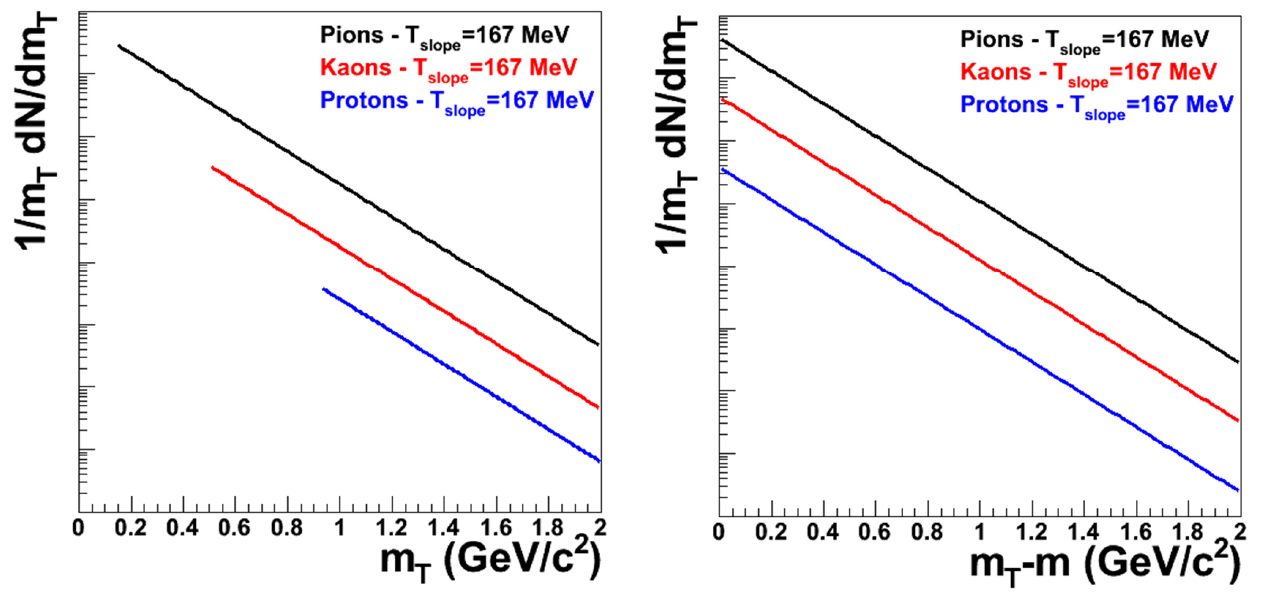
\includegraphics[scale=0.3]{figures/mt.png}\label{fig:mtd}}\quad
  \subfloat[][]
  {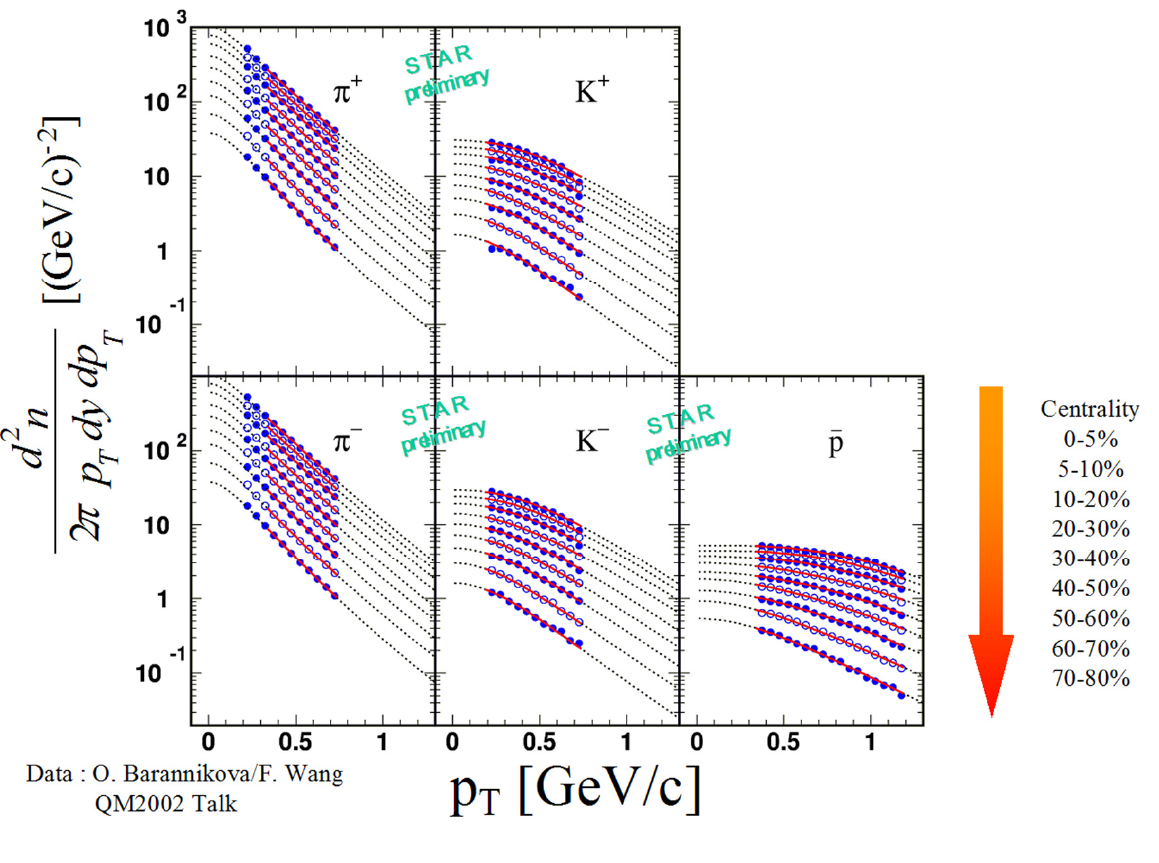
\includegraphics[scale=0.35]{figures/breakscale.png}\label{fig:breakscale}}
  \caption{(a) $m_{T}$ spectra for different particles in p-p collisions. (b) $m_{T}$ spectra for different particles in AA collisions for different values of centrality at the STAR experiment.}
\end{figure}
%
However, in nuclei collisions the $m_{T}$ is broken. In facts, as it can be seen in Figure \ref{fig:breakscale}, the slope of the spectra decreases when the mass of the particle increases, i.e. the heaviest particles are shifted to higher values of $p_{T}$, and $T_{slope}$ has a linear dependence on the mass of the particle. This phenomenon can be explained introducing a collective motion of all the particles, superposed to the thermal motion:
\begin{equation}
 T_{slope}\;=\;T_{fo} + \frac{1}{2}mv_{\perp}^{2}.
\end{equation}
This collective expansion in the transverse plane is called radial flow. This collective motion is generated by the high pressures generated when the nuclear matter is compressed and heated and, in the case of central collisions, this flow is characterized by a circular symmetry on the azimuthal angle in the transverse plane.\\
Fitting the spectra of identified particles, it is possible to separate the thermal component from the collective one, obtaining the freeze-out temperature $T_{fo}$ and the radial speed $\beta_{\perp}$. At the ALICE experiment, the temperature of the thermal freeze-out is $T_{fo} \approx$ 110 - 130 MeV.\\
\subsubsection{Anisotropic flow}
While in central collision the radial flow is characterized by an azimuthal symmetry in the transverse plane, fer semi-central collisions the overlap between the colliding nuclei has an asymmetric almond shape, so the pressure gradients inside the generated medium lead to anisotropies in $\phi$. In facts, the impact parameter generates a favoured direction in the transverse plane: the impact parameter and the beam direction define the so called \textit{reaction plane}, identified by the angle $\Psi_{RP}$ in the transverse plane.\\
%
\begin{figure}
  \centering
  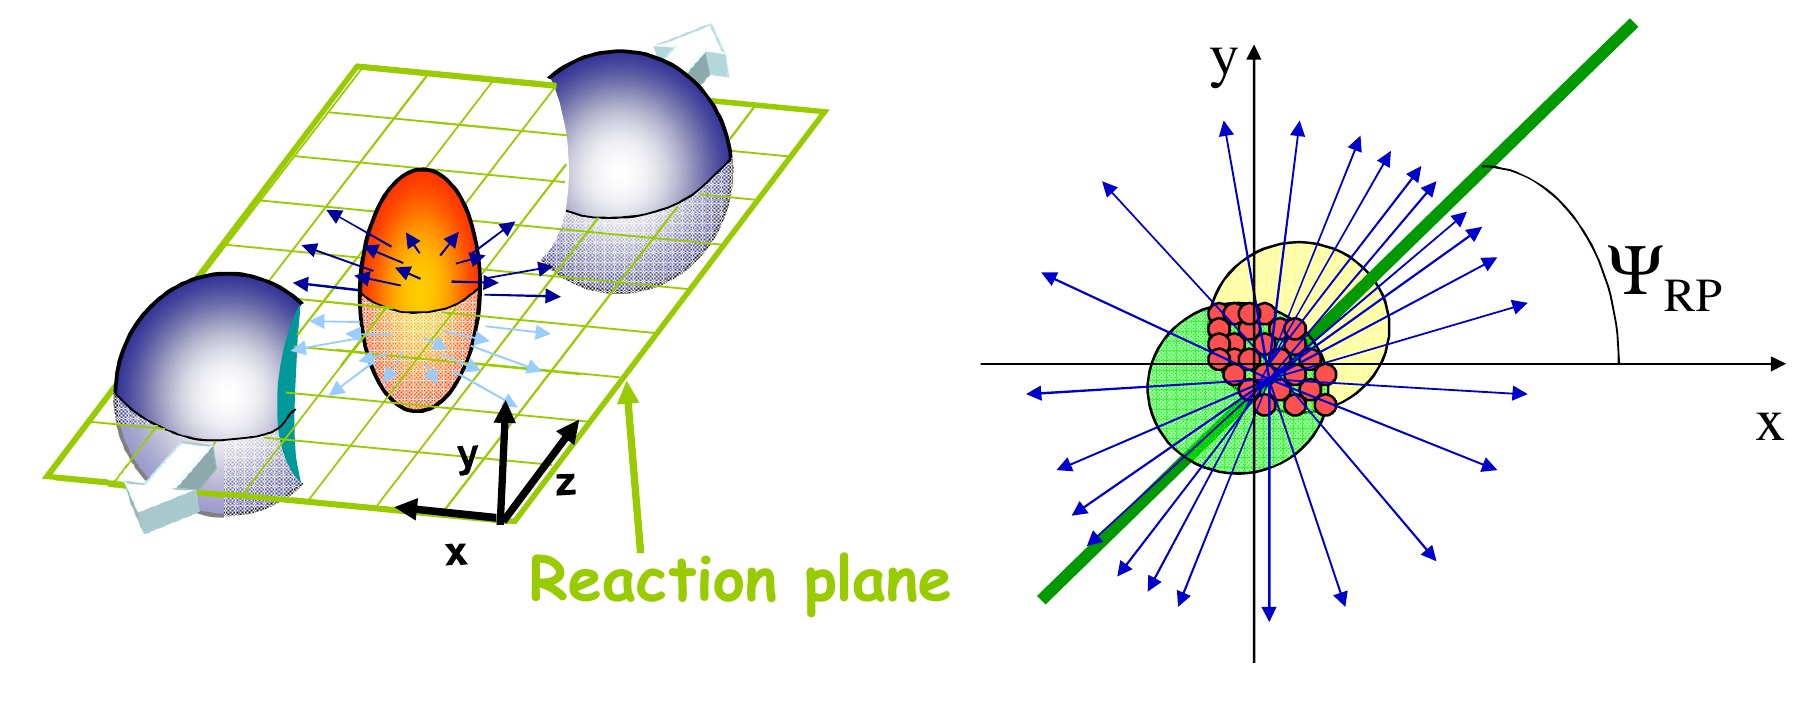
\includegraphics[scale=0.3]{figures/flow.png}
  \caption{Anisotropic flow and reaction plane definition.}
  \label{fig:flow}
\end{figure}
%
There are both spatial anisotropies and momentum anisotropies: the interactions among the particles, if strong enough, can convert the initial geometrical anisotropy into an anisotropy in the momenta distribution, that can be measured.\\
The azimuthal particle distribution can be parametrized with a Fourier expansion:
\begin{equation}
 \frac{dN}{d(\phi-\Psi_{RP})}\;=\;\frac{N_{0}}{2\pi} + \frac{N_{0}}{\pi}\sum_{z} \nu_{k}\cos[k(\phi-\Psi_{RP})]
\end{equation}
In this equation, the sine functions are not present, since the distribution must be symmetric with respect to $\Psi_{RP}$.
The coefficients of the harmonics, which are given by the expression:
\begin{equation}
 \nu_{k}\;=\;\langle \cos[k(\phi-\Psi_{RP})]\rangle,
\end{equation}
describe different kinds of anisotropies: $\nu_{1}$, for example, is the \textit{direct flow} coefficient and describes an asymmetry between forward and backward particle production; $\nu_{2}$, instead, is the elliptic flow, which describes the difference between the number of particle emitted in the reaction plane and in the direction orthogonal to it. For the other coefficients, the situation is similar.\\
The geometrical anisotropy, which is the origin of the elliptic flow, attenuates with the evolution of the system, since the gradients of pressure, which are responsible for this asymmetry, are stronger in the first instants of the collision. Therefore, the measurement of the elliptic flow allows to get information about the state equation of the system in the early stages of the collision, being a good test for hydrodynamic models which describe the evolution of the medium. According to the to the measure of the anisotropic flow, the QGP seems to behave like a perfect fluid, rather than like a perfect gas, as one could expect.\\
\subsection{Nuclear modification factor}
The remaining observables used at the ALICE experiment are hard probes, i.e. particles generated in the first stages of the collision, in processes with an high momentum transfer. For this reason, hard probes can give important information about the properties of the medium, even if they are rare events (< 0.1\%).\\
In order to understand the differences between p-p and nuclei collision, it is important two compare the results of the formers with those of the latters.\\
In nuclei collisions the probability of interaction, according to the Glauber Model, scales with the number of elementary nucleon-nucleon collision $N_{coll}$:
\begin{equation}
 p_{AA}^{hard}\;\propto\;\sigma_{hard}N_{coll}
\end{equation}
For this reason, it is expected that transverse momentum spectra measured in nuclei collision can be obtained scaling the spectra for p-p collisions by the the number of elementary collisions $N_{coll}$.
Therefore, the \textit{nuclear modification factor}  can be defined as:
\begin{equation}
 R_{AA}(p_{T})\;=\;\frac{1}{\langle N_{coll}\rangle}\frac{dN_{AA}/dp_{T}}{dN_{pp}/dp_{T}}.
\end{equation}
For low values of the transverse momentum ($p_{T} \lesssim$ 2 GeV), $R_{AA}$ < 1 is expected, since the probability for soft processes, according to the Glauber model, scales with the number of participants $N_{part}$. For hard particles, instead, $R_{AA} \sim$ 1 is expected. It is important to note that heavy quarks (c, b, t) belong to hard physics independently from the transverse momentum value, because their high masses can be produced only in processes with a high momentum transfer. In reality, for values of $p_{T} \gtrsim$ 2 GeV, the $R_{AA}$ is greater than the unity, thanks to phenomena like the Cronin effect, i.e. a translation of the $p_{T}$ spectra towards higher values, due to multiple interactions of the nucleon inside the other nucleus, and the modification of the parton distribution functions. These are called initial states effects because they are not influenced by the evolution of the system, but depend on initial conditions. The $R_{AA}$ can also be modified by final state effects, which reflect the interaction of the particles with the medium generated in the collision. Indeed, since high momentum partons are created in the first stages of the collision, they undergo all the evolution of the collision and their momentum can change due to the energy loss in the fireball, which could lead to the quenching of high $p_{T}$ spectra. The energy loss can be evaluated from the \textit{BDMPS formula}[da mettere]:
\begin{equation}
 \langle \Delta E \rangle \;\propto\;\alpha_{S} \:C_{R}\: \hat{q}\: L^{2},
\end{equation}
where $\alpha_{S}$ is the QCD coupling constant, $C_{R}$ is the Casimir factor, whose value is 4/3 for a quark-gluon coupling and 3 for a gluon-gluon 
one, $\hat{q}$ is the transport coefficient, related to the properties of the medium and proportional to the density and the momenta of the gluons. \textit{L}, finally, is the distance travelled by the particle in the medium. This formula parametrizes the energy loss through the emission of gluons and this gives an explanation of the dependence from $L^{2}$, since the gluons can also interact with the medium.\\
In the next sections, the main hard probes observed at ALICE will be described.\\
\subsection{Jet quenching}
A jet is a collimated emission of hadrons, which originates from fragmentation of a high-$p_{T}$ parton. These partons are created back to back in the initial collision and they form hadrons during the hadronization. For this reason, in small systems, such as in p-p collisions, two jets of hadrons emitted in opposite directions are usually seen. In ion collisions, however, the situation in different, since the high energy parton can interact with the medium and, consequently, lose energy as previously described.
%
\begin{figure}
  \centering
  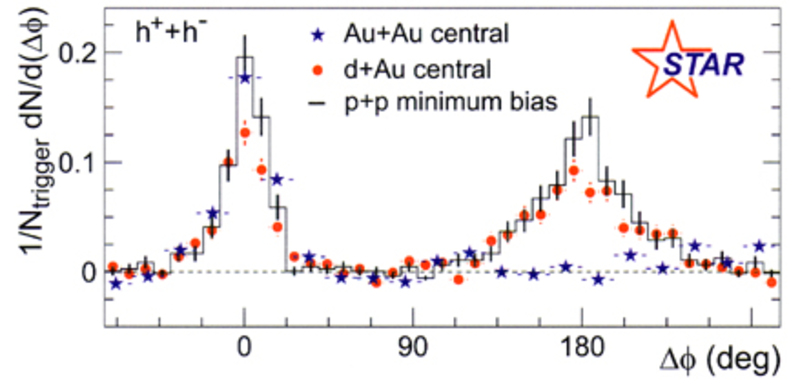
\includegraphics[scale=0.3]{figures/zoom.jpeg}
  \caption{Azimuthal distributions for p-p, d-Au, Au-Au at STAR \cite{jets}.}
  \label{fig:jet}
\end{figure}
%
Hence, for ion collisions, the azimuthal distribution of high momentum particles is strongly dependent on the point of creation of the pair $q\bar{q}$. Indeed, if the partons are produced inside the fireball, they are slowed down while exiting the medium and so they hadronize in low $p_{T}$ particles. Otherwise, if the pair is produced on the surface of the fireball, the hadron whose momentum is directed outwards hadronizes in a high $p_{T}$ particle, i.e. creates a jet that can be detected, while the parton emitted inwards travels through the whole fireball, losing energy and hadronizing in a low $p_{T}$ particle. Therefore, the study of azimuthal angle correlation between two high $p_{T}$ particles can give important information about the creation of a hot and dense medium.\\
In Figure \ref{fig:jet}, the measures of the azimuthal correlation are reported for p-p, d-Au and Au-AU collisions for the STAR experiment. As it can be seen, for the first two kinds of collision there are two jets emitted back to back, while for heavy ions collisions one of the jets is suppressed. This can be considered a proof of the creation of a hot and dense medium, such as the QGP.\\
\subsection{Open heavy flavours}
Particles constituted by a heavy quark, i.e. charm and beauty, are called \textit{open heavy flavours}. Considering the great mass value of the heavy quarks ($m_{b}\sim$ 4.8 GeV and $m_{c}\sim$ 1.2 GeV), they can only be produced in the initial stages of the collision, in scatterings with a high momentum transfer between partons. For this reason, their production con be described using the perturbative QCD till very low values of transverse momentum. This kind of measurements is used both in p-p collisions, in order to test the theoretical model based on the perturbative QCD and to have a reference for the $R_{AA}$ determination, and in heavy ion collisions, in order to test the energy loss models.\\
In particular, the energy loss models predict a different loss for hadrons containing heavy quarks compared to light hadrons. This is explained with the different origin of the two types: heavy flavours are generated from a quark fragmentation, while light flavours are mainly produced from gluons. Then, the is the so called \textit{dead cone effect} \cite{deadcone}: the gluon radiation is suppressed at small angles (with respect to the direction of motion) for heavy quarks. In particular, being $E_{Q}$ and $M_{Q}$ respectively the energy and the mass of the heavy quark, the suppression is predicted for angles $\theta<\frac{M_{Q}}{E_{Q}}$. Therefore, the energy loss for light flavours is bigger than in heavy flavours, and the energy loss loss of a particle with a charm quark is bigger than that of a particle with a beauty. The measures of $R_{AA}$ seem to confirm this behaviour for charmed and beautied particles, but higher statistics is needed in order to see the difference between charmed particles and light flavours.\\
\subsection{Heavy quarkonia suppression}
Another hard probe of the QGP is given by the heavy quarkonia, i.e. bound states made of a heavy quark and the respective antiquark: charmonium ($c\bar{c}$) and bottomonium ($b\bar{b}$). Since they are composed of heavy quarks, they have been generated in the first stages of the collision. However, the quarks in this bound states are characterized by a non relativistic motion ($\beta\sim$ 0.4) and so the system cannot be described using a perturbative approach.\\
In the vacuum, the binding potential of a quarkonium state can be expressed using the Cornell potential:
\begin{equation}
 V(r)\;=\;-\frac{\alpha_{S}}{r}+kr,
\end{equation}
where \textit{k} is a parameter and \textit{r} is he distance between \textit{q} and $\bar{q}$.
As it can be seen, this potential is composed of a coulombian potential, induce by the exchange of a gluon, and a confining potential, which parametrizes the non perturbative effects.\\
However, if the quarkonium is immersed in the QGP, the binding potential changes, since the presence of free quarks and gluons act as a screen bewteen the pair $q\bar{q}$. Therefore, in this case the potential becomes a Yukawa type potential:
\begin{equation}
 V(r)\;=\;-\frac{\alpha_{S}}{r}e^{-\frac{r}{\lambda_{D}}}.
\end{equation}
The quantity $\lambda_{D}$ is called \textit{Debye length}, and is related to the the longest distance at which two colour charges can form a bound state in a QGP. An expression for the Debye length can be obtained from leading order calculations in perturbative QCD:
\begin{equation}
 \lambda_{D}\;=\;\frac{1}{g\sqrt{\frac{N_{c}}{3}+\frac{N_{f}}{6}}T},
\end{equation}
where $N_{c}$ is the number of colours and $N_{f}$ is the number of flavours.\
The Debye length, hence, decreases when the temperature increases and, consequently, it is possible to determine the temperature of the QGP from the presence or the suppression of a particular excited state of quarkonia. In facts, states which are more bounded have smaller dimensions and, for this reason, they survive at higher temperatures.\\
The idea of using the $J/\Psi$ suppression as a signature of the QGP formation was introduced in 1986 by Matsui and Satz, in one of the most famous articles of the ultra-relativistic ion physics \cite{matsui}.\\
%
\begin{figure}
  \centering
  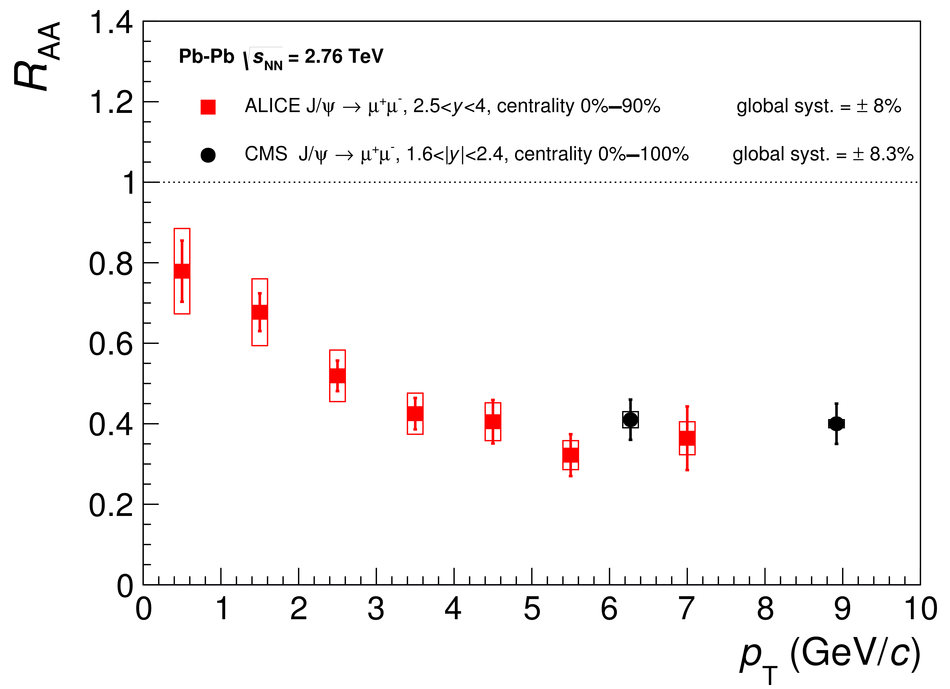
\includegraphics[scale=0.25]{figures/jpsi.png}
  \caption{Transverse momentum dependence of the centrality integrated $J/\Psi$ $R_{AA}$ measured by ALICE in Pb-Pb collisions at $\sqrt{s_{NN}}$ = 2.76 GeV compared to CMS results at the same $\sqrt{s_{NN}}$.}
  \label{fig:jpsi}
\end{figure}
%
\chapter{The ALICE Experiment}
%\lettrine{A}
ALICE (\textit{A Large Ion Collider Experiment}) is one of the four major experiments at the \textit{Large Ion Collider}, at CERN, in Geneva. It was expressly designed to study heavy ion collisions, continuing the tradition of experiments such as STAR and PHENIX at RHIC, but also experiments held at SPS and AGS before. The aim of the experiment is the study of the QGP, using Pb-Pb collisions. ALICE has also a program with data from pp and p-Pb collisions, needed to discern final state effects from initial states effects.\\
In this chapter a description of the experimental set up will be given, focusing on the \textit{Inner Tracking System}, the detector on which this work is based, after a brief introduction about the LHC.
\section{Large Hadron Collider}
%
\begin{figure}
  \centering
  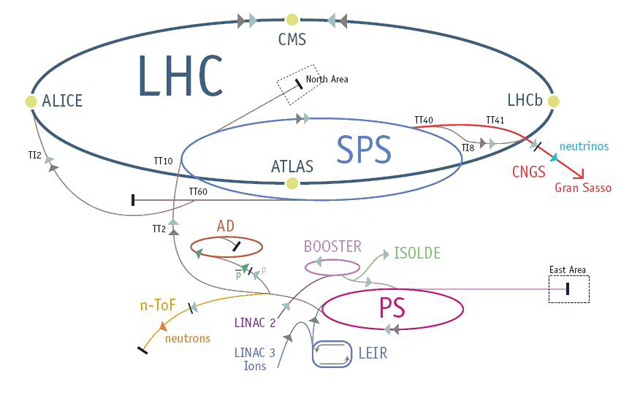
\includegraphics[scale=0.55]{figures/LHC.jpg}
  \caption{The accelerator complex at CERN.}
  \label{fig:LHC}
\end{figure}
%
The LHC is the world's largest and most powerful accelerator \cite{lhc}. It consists of a 27 km ring of superconducting magnets with a number of accelerating structures to boost the energy of the particles up to their collision energy and keep them stable, compensating the energy loss. The LHC is designed to deliver pp collisions at $\sqrt{s}$ = 14 TeV, with a rate of 40 MHz, and Pb-Pb collisions at $\sqrt{s_{NN}}$ = 5.5 TeV, with a rate of 8 kHz. However, in the first run the LHC did not work at the highest energy, collecting mainly data for pp collisions at $\sqrt{s}$ = 7 TeV and Pb-Pb collisions at $\sqrt{s_{NN}}$ = 2.76 TeV. In the second run, instead, the LHC is working at the design energies.\\
In Figure \ref{fig:LHC} a schematic view of the accelerator complex of CERN is shown. Protons and lead ions pass through different processes before reaching the LHC. Starting from protons, they are extracted from an hydrogen tank and injected in the linear accelerator LINAC2, where they reach an energy of 50 MeV. Then, they are accelerated to 1.4 GeV in the \textit{Proton Synchrotron Booster} (PSB) and injected in the \textit{Proton Synchrotron}, where they reach an energy of 25 GeV. Then, in the \textit{Super Proton Synchrotron} (SPS) they reach 450 GeV and are finally injected in the LHC. For lead ions the process is different, in particular in the initial steps. First of all, lead (Pb$^{208}$) ions are extracted from a purified sample of lead brought to high temperatures ($\sim$ 500 \textdegree C) thanks to microwaves and the partially ionized by a stream of electrons, creating ions with different charges, among which only Pb$^{29+}$ are selected. After being accelerated in LINAC3 at 4.2 MeV per nucleon, more electrons are stripped by passing through a carbon foil. Only Pb$^{54+}$ are kept end then accelerated in the \textit{Low Energy Ion Ring} (LEIR) at 5.9 MeV. Afterwards the ions are transferred to the PS, where they reach the energy of 5.9 GeV per nucleon end then pass through a copper foil, being fully stripped. The beam of Pb$^{82+}$ is then injected in the SPS (177 GeV per nucleon) and finally in the LHC, where they reach their final energy.
\section{Design considerations for ALICE}
The multiplicity of produced particles is a very important characteristic in the heavy ion collision experiments. For these kinds of studies, indeed, it is important to track and identify all the particles coming from the interaction region, in order to measure the quantities described in the previous chapter. As already mentioned, the ALICE experiment was designed when RHIC data were not available yet, and the estimated multiplicity for heavy ion collision at the energy of the LHC was 2000 - 6000 charged particles per rapidity unit. Consequently, the ALICE experiment has been designed in order to bear a multiplicity of 8000 particles per rapidity units. When the RHIC measurements became available, they showed that the multiplicity range at LHC should have been 1500 - 4000 particles for rapidity unit. Therefore, the designed was optimized for $\frac{dN}{dy}\sim$ 4000. The low interaction rate for heavy-ion collisions allows to use slow detectors, such as the time projection chamber and the silicon drift detectors, which are very suitable for the particle identification even at a high value of multiplicity.
Another important parameter that has been taken into account in the design of the experiment is the product of the efficiency, defined as the ratio between detected particles and generated particles, by the acceptance. ALICE is hermetic in $\varphi$, i.e. it covers $2\pi$ radians in the azimuthal angle.\\
ALICE, moreover, has been designed to work on a wide $\pt$ range. Thanks to the mild magnetic field (0.5 T), it is possible to track particles down to very low values of transverse momentum (tens of MeV). This feature is ideal for the study of particles with low momentum, but the combination of the chosen magnetic field with the long lever arm of the detector allows precise momentum measurements even at high momentum ($\pt\lesssim$ 100 GeV/c).\\
Beside the reconstruction of the trajectories of the charged particles, the particle identification (PID) is extremely important to reconstruct the particle spectra. At the ALICE experiment, the identification of particles with low transverse momentum ($\pt$ < 4 GeV/c) is performed in the central barrel ($|\eta|$ < 0.9). For higher momenta, the particle identification can be done just in a restricted range of $\eta$ and $\varphi$ by specialized detectors.
\section{ALICE experimental apparatus}
%
\begin{figure}
  \centering
  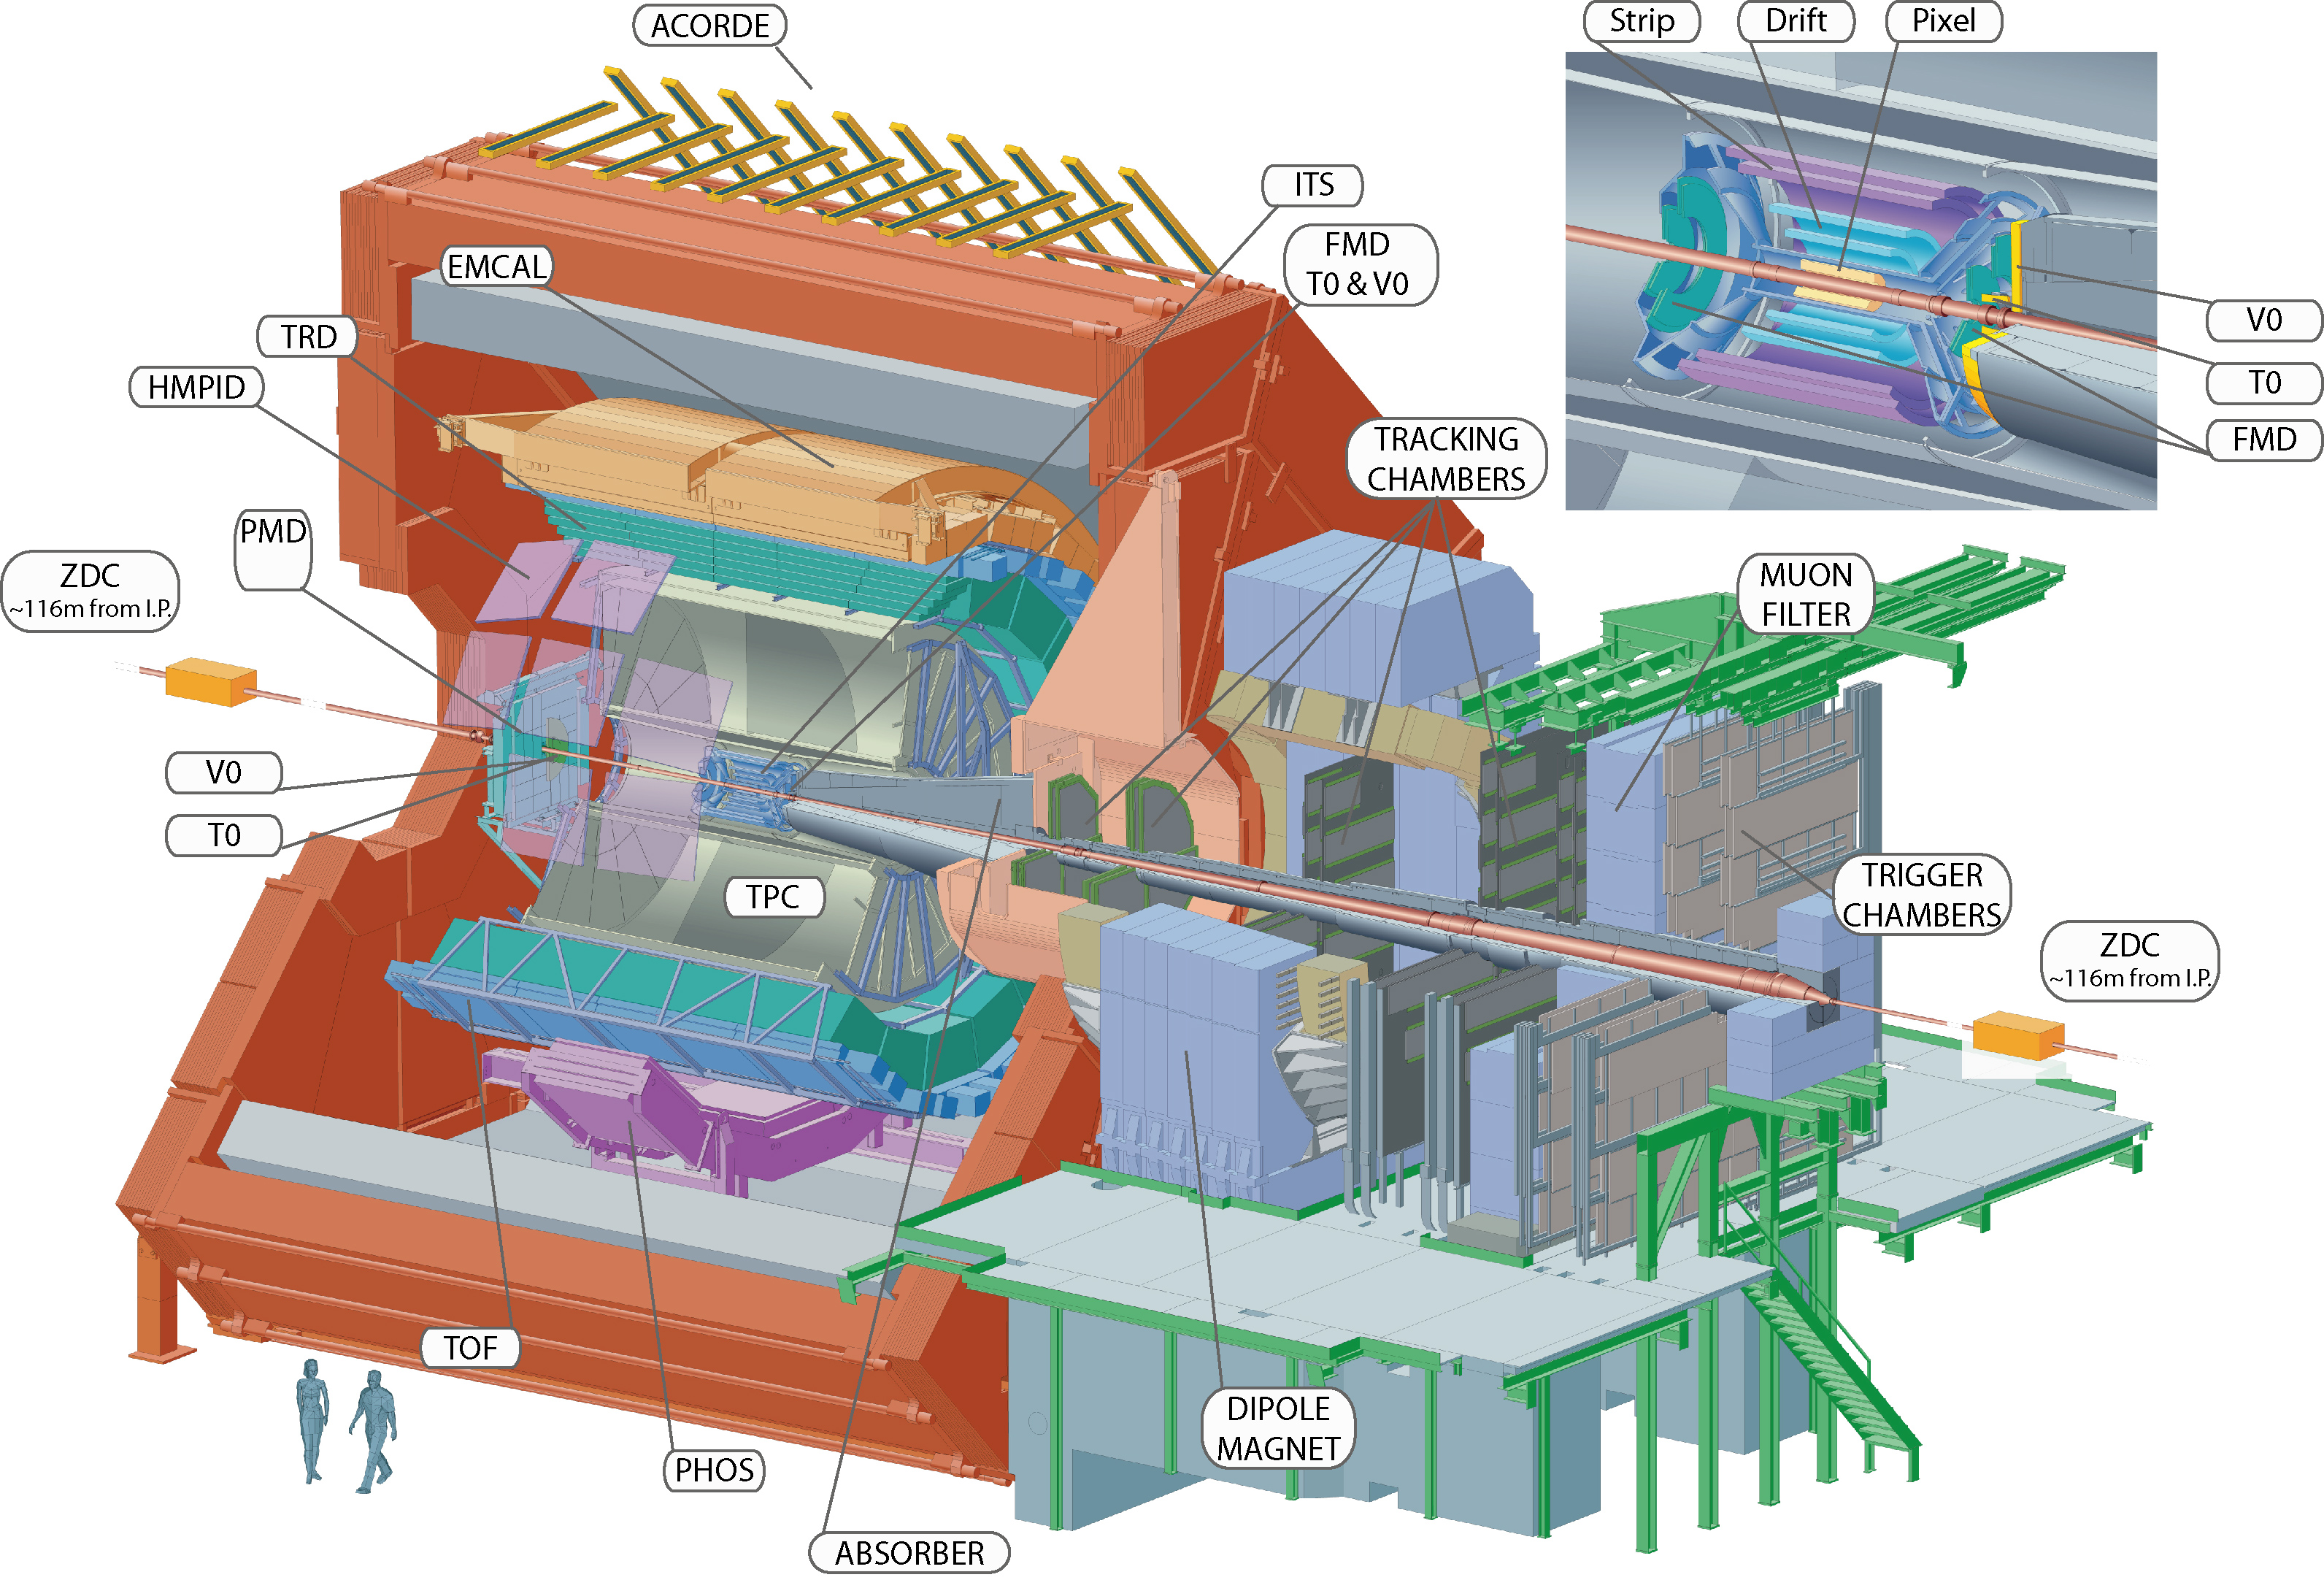
\includegraphics[scale=0.55]{figures/ALICEapp.jpg}
  \caption{The ALICE experimental setup.}
  \label{fig:ALICEapp}
\end{figure}
%
The experimental setup of ALICE is shown in figure \ref{fig:ALICEapp}. It is composed of three main parts: the \textit{central barrel}, which covers the mid-rapidity region (|$\eta$|<0.9), the \textit{muon arm}, which covers the forward pseudorapidity range -4 $\leq \eta \leq$ -2.5, and the \textit{forward detectors}.\\
All the detectors in the central barrel are immersed in the magnetic field of 0.5 T, generated by the ALICE solenoid magnet, used previously in the L3 experiment at the Large Electron-Positron (LEP) collider. The detectors of the central barrel, starting from the beam line and going outwards, are: the \textit{Inner Tracking System} (ITS), the \textit{Time Projection Chamber} (TPC), the \textit{Transition Radiation Detector} (TRD), the \textit{Time Of Flight} (TOF), the \textit{High Momentum Particle IDentification} detector (HMPID), the \textit{PHOton Spectrometer} (PHOS), the \textit{ElectroMagnetic Calorimeter} (EMCal) and the \textit{ALICE COsmic Ray DEtector} (ACORDE).\\
In the muon arm there is the \textit{Muon Spectrometer}, a forward detector which lays outside the solenoid magnetic field.\\
Finally the forward detectors, which are located at a small angle with respect to the beam line, include the \textit{Zero Degree Caloremeter} (ZDC), the \textit{Photon Multiplicity Detector} (PMD), the \textit{Forward Multiplicity Detector}, the \textit{VZERO} detector (V0) and the \textit{TZERO} (T0).\\
All these detector will be described in the next sections, after the description of the coordinate system.
\subsection{ALICE coordinate system}
The ALICE coordinate system is a right-handed Cartesian system with the origin at the nominal beam interaction point. The axes are defined as follows:
\begin{itemize}
 \item \textit{x axis:} it is perpendicular to the mean beam direction, aligned with the local horizontal and pointing to the centre of the LHC;
 \item \textit{y axis:} it is perpendicular to the x axis and the beam direction, pointing upwards;
 \item \textit{z axis:} it is parallel to the beam direction, with the positive direction opposite to the Muon Spectrometer (ATLAS side).
\end{itemize}
\subsection*{Magnets}
The central barrel detectors are embedded in a magnet that is a room temperature solenoid magnet, which generates a moderate magnetic field of 0.5 T. This kind of magnetic field has been chosen since it is intense enough to bend the trajectories of the particles but mild enough to allow the reconstruction of low momentum particles in the TPC. In the TPC it is possible to track particles with a transverse momentum larger than $p_{cut-off} = 0.3 BR \sim$ 0.2 GeV/c, where B is the magnetic field in Tesla, and R = 2.5 m is the external radius of the TPC. However, particles with lower momentum ($\gtrsim$ 100 MeV/c \cite{raro}) can be tracked using the ITS stand-alone.\\
A dipole magnet is placed at 7 m from the interaction vertex along the z direction. It generates a field of 0.2 T, perpendicular to the beam direction that is used as bending field to measure the momentum of muons in the Muon Spectrometer.
\subsection*{Inner Tracking System}
The ITS is the closest detector to the interaction point and is composed of six layers of silicon detectors of different technologies. Its main uses are the location of the primary vertex, i.e. the collision point, with a resolution better than 100 $\mu$m, the reconstruction of the secondary vertices of the decays of the heavy flavoured hadrons and hyperons and the tracking and the identification of low-$\pt$ particles ($\pt \gtrsim$  100 MeV/c). It also improves the momentum and angle resolution for tracks reconstructed by the TPC and allows the reconstruction of particles which traverse dead regions of the TPC. It also gives information about the particle energy loss in the four outer layers. A more detailed description of the ITS will be given later in a dedicated section.
\subsection*{Time Projection Chamber}
%
\begin{figure}
  \centering
  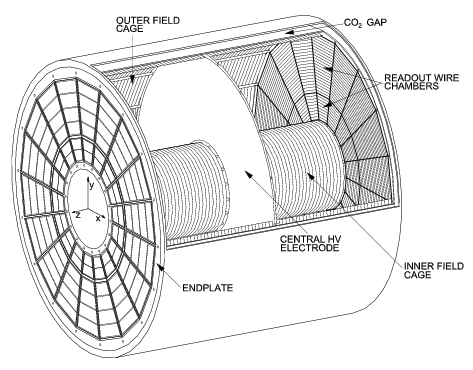
\includegraphics[scale=0.5]{figures/tpc.png}
  \caption{The setup of the TPC.}
  \label{fig:TPC}
\end{figure}
%
The TPC is the main tracking detector of the central barrel. It is optimised to provide momentum measurements with good two-track separation, particle identification via \textit{dE/dx} and vertex determination together with the other detectors of the central barrel. The TPC covers the pseudorapidity range |$\eta$| < 0.9 for tracks with full radial length, i.e. with matches in ITS, TRD and TOF detectors. The 2$\pi$ acceptance in the azimuthal angle is guaranteed by its cylindrical symmetry. The total active volume has an inner radius of 85 cm, an outer radius of 250 cm and a total length along the beam direction of 500 cm. The detector is made of a cylindrical field cage, with a central high-voltage electrode and two opposite axial potential dividers to create a highly uniform electric field. The cavity is filled with 90 m$^3$ of Ne/CO$_2$/N$_2$ (90/10/5).\\
When a charged particle passes through the TPC ionizes the gas creating electron-ion pairs. Thanks to the uniform electric field, the electrons drift towards the end-plates, where they are detected.
The gas mixture is therefore optimised for drift speed, low diffusion, low radiation length and hence low multiple scattering, small space charge effects and stability properties. In particular the N$_2$ improves the quenching of the electron multiplication, keeping the proportionality of the signal to the energy deposit of the charged particles and allowing a higher maximum gas gain. As far as the Ne/CO$_2$ is concerned, the drift speed is strongly dependent on its temperature and therefore a high thermal stability is required ($\Delta$T $\leq$ 0.1 K).\\
In the end-plates the electrons are detected by multi-wire proportional chambers with cathode pad readout, providing the position in the transverse plane. The information about the z position is provided by the measure of the drift time, for which it is necessary to use a trigger information from an external detector, like the V0. The position resolution is different  along the radial direction because of the different track density: for the inner/outer radii is 1100/800 $\mu$m in the transverse plane and 1250/1100 $\mu$m along the beam axis.
%
\begin{figure}
  \centering
  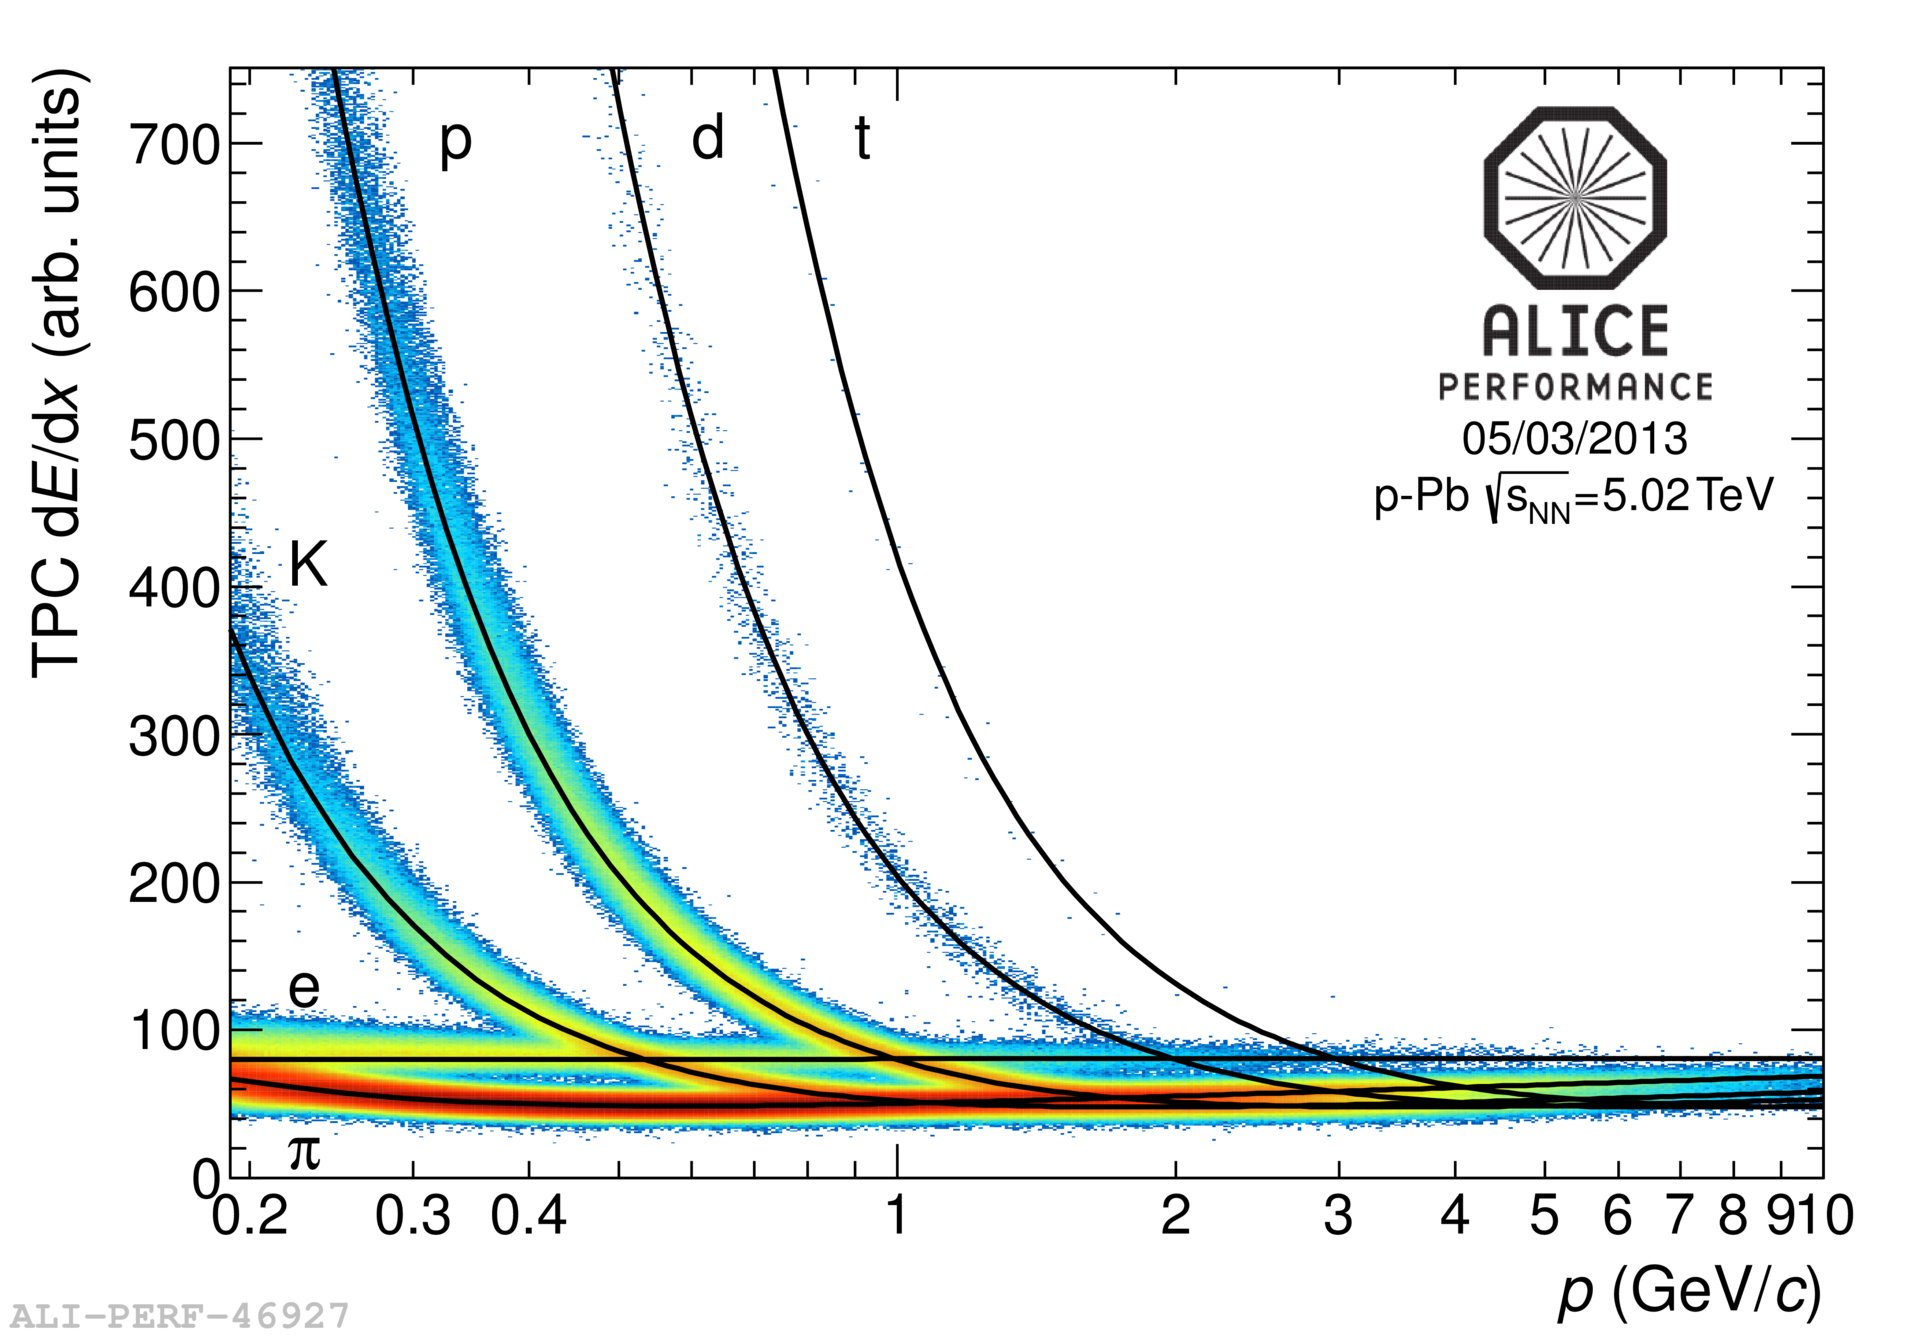
\includegraphics[scale=0.15]{figures/TPC_Perf.png}
  \caption{\textit{dE/dx} of charged particles vs their momentum measured by the TPC in p-Pb collisions. The lines are a parametrization of the detector response based on the Bethe-Bloch formula \cite{alice2014performance}.}
  \label{fig:TPC_Perf}
\end{figure}
%
The total charge collected at the end-plates is proportional to the energy loss of particles in the gas mixture and therefore the PID is possible via \textit{dE/dx}. In particular the \textit{dE/dx} resolution is 5\% for isolated tracks and 6.8\% in case of high occupancy. From \textit{dE/dx} measurements it is possible to identify different particles species in the momentum region where their \textit{dE/dx} are separated. This separation is better at low momentum (p $\lesssim$ 1 GeV/c), where the bands are more distant, but it is possible also at large values of the momentum (p $\gtrsim$ 4 GeV/c) thanks to the relativistic rise of \textit{dE/dx} in the TPC gas.\\
The TPC is a very good detector for tracking and PID, but the large drift time (88 $\mu$s), of the order of 10$^{-3}$, is a great limit for the data acquisition rate.\\
\subsection*{Transition Radiation Detector}
The TRD is used for identifying electrons with momentum above 1 GeV/c, for which the identification in the TPC by measuring the \textit{dE/dx} is no longer efficient. This detector is composed of 540 individual readout detector modules, with an inner radius of 2.9 m and an outer radius of 3.68 m. It works in the pseudorapidity range |$\eta$| < 0.84. The TRD is important, for example, for the separation of the electrons from the J/$\Psi$ decay from the background of Dalitz decays. Moreover combining the information about the impact parameter from the ITS and the identification from the TRD it is possible to study charmed particles with decaying in their semi-leptonic channels. The TRD is composed of radiators in which photons are emitted at charged particle passage and of wire chambers filled wit Xe/CO$_2$. It is suitable for the identification of particles with a Lorentz $\gamma$ larger than 1000 and for this reason it can separate well electrons and pions whose momentum is in the range 1 GeV/c $\leq$ p $\leq$ 100 GeV/c.
\subsection*{Time Of Flight}
The TOF detector consists of a large area array of Multi-gap Resistive Plate Chambers (MRPC) in the central pseudorapidity range (|$\eta$| < 0.9). It is used for the PID in the intermediate momentum range, up to 2.5 GeV/c for pions and kaons, up to 5 GeV/c for protons. It has a cylindrical symmetry like the TPC, with an internal radius of 370 cm, an external one of 399 cm and a total length of 7.45 m. The thickness of the whole detector corresponds to 30\% of a radiation length. When a charged particle passes through the detector ionizes the gas creating an electron avalanche which is collected by the electrodes. The avalanche regime is possible thanks to the high electric fields inside the MWPC.\\
%
\begin{figure}
  \centering
  \includegraphics[scale=0.15]{figures/TOF.png}
  \caption{$\beta$ vs momentum of charged particles measured by the TOF in p-Pb collisions \cite{alice2014performance}.}
  \label{fig:TOF}
\end{figure}
%
The PID is based on the measure of the time of flight of a particle from the interaction point to the TOF detector. Using the track length measured with the ITS and the TPC and using as initial time the time of particle production, provided by the T0 detector, it is possible to measure the $\beta$ of the particle and, considering the momentum measure of the TPC, to identify the particle itself.\\
\subsection*{High Momentum Particle Identification Detector}
\begin{figure}
  \centering
  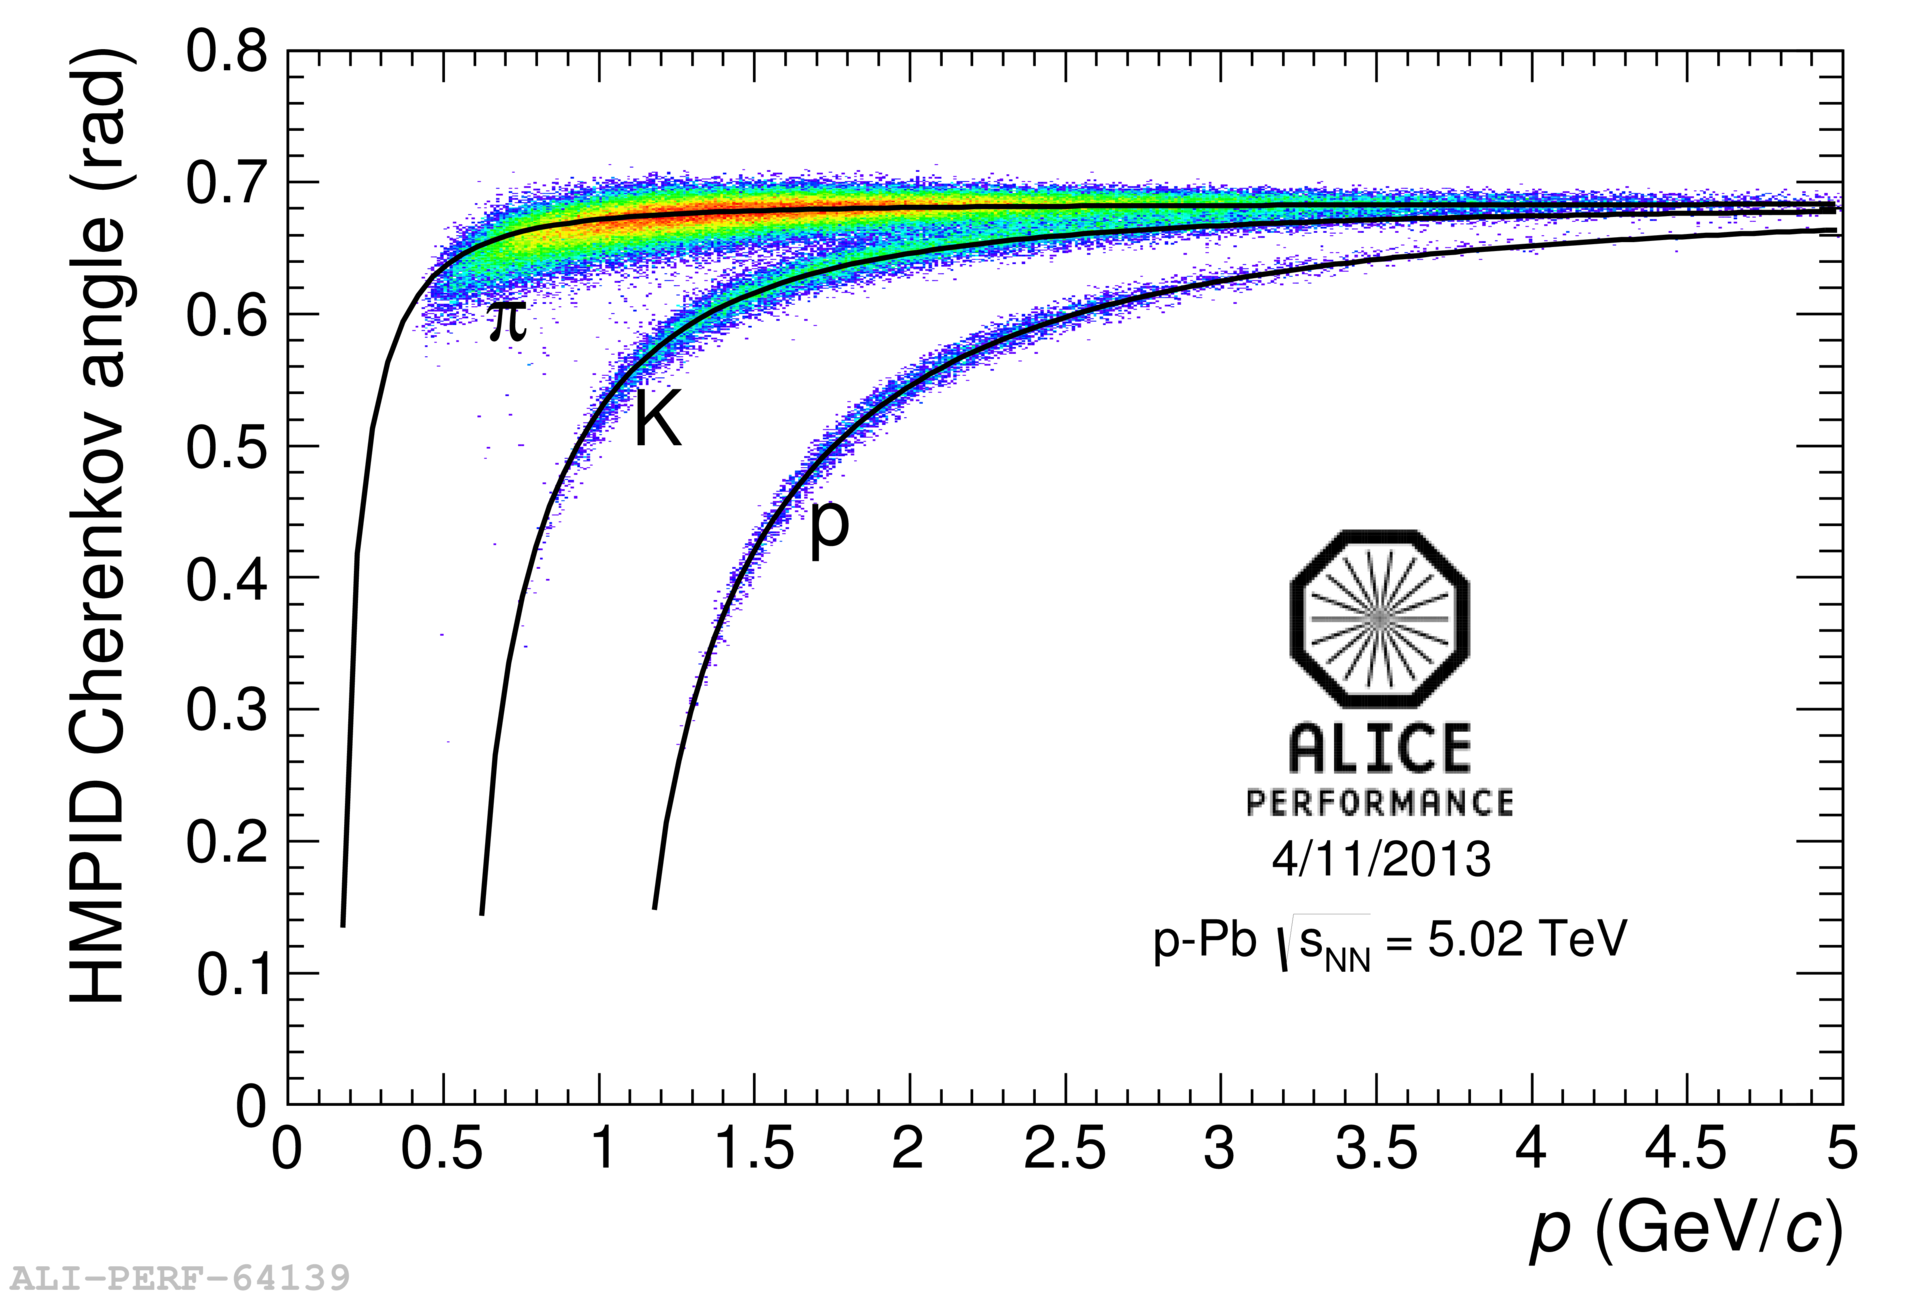
\includegraphics[scale=0.15]{figures/HMPID.png}
  \caption{HMPID Cherenkov angle vs track momentum for p-Pb @ 5.02 TeV data, Continuous lines represent theoretical Cherenkov angle values vs track momentum \cite{alice2014performance}.}
  \label{fig:HMPID}
\end{figure}
%
The HMPID is dedicated to the identification of hadrons at $\pt$ > 1 GeV/c, enhancing the PID capability of ALICE beyond the momentum interval attainable with ITS, TPC and TOF. In particular it has been optimized to extend the range for $\pi$/K and K/p discrimination respectively up to 3 GeV/c and 5 GeV/c. It is characterized by a small acceptance, 5\% of central barrel phase space, covering the pseudorapidity range |$\eta$|<0.6 and the azimuthal angle range 1.2\textdegree < $\varphi$ < 58.8\textdegree. The HMPID is based on proximity-focusing Ring Imaging Cherenkov (RICH) and consists of seven modules of about 1.5 $\times$ 1.5 m$^2$ each, mounted at a distance of about 5 m from the beam line. When a charged particle passes through the radiator, filled with liquid perfluorohexane (C$_6$F$_{14}$), with a speed higher than the speed of light in the medium, Cherenkov photons are emitted. The Cherenkov photons are then detected by a photon counter made of CsI scintillators and a MWPC with pad cathode.
\subsection*{Photon Spectrometer}
The main physics objective of the PHOS is the test of thermal and dynamical properties of the initial phase of the collision through the measurement of low $\pt$ direct photons and of the jet quenching, which can be obtained observing high-$\pt$ $\pi^0$ and $\gamma$-jet correlations. In order to distinguish the direct photons from those generated in $\pi^0$ and $\eta$ decays, good spatial and energetic resolution are needed. The detector consisted of five modules of lead-tungstate crystals (PbWO$_4$) and it is located at 4.6 m from the beam line. It has a low acceptance, covering the pseudorapidity range |$\eta$|<0.12 and the azimuthal angle range 220\textdegree < $\varphi$ < 320\textdegree.
\subsection*{Electromagnetic Calorimeter}
The main goal of the EMCal is to enhance ALICE performances in the the study of the jet production in Pb-Pb collisions. It extends the ALICE capabilities in detecting direct photons, jets and the electrons from heavy flavoured hadron decays. It provides complementary measurements to the PHOS, being positioned approximately in the opposite side, at a radius of about 4.5 m, adjacent to the magnet. It covers the pseudorapidity range |$\eta$|<0.7, with an azimuthal angle range $\Delta\varphi$ = 107\textdegree. The detector is a layered Pb-scintillator sampling calorimeter, alternating 1.44 mm of lead and 1.76 mm of polystyrene.
\subsection*{ALICE Cosmic Ray Detector}
The ACORDE is an array of plastic scintillator counters placed on the upper surface of the L3 magnet and is used for the cosmic ray detection. It covers |$\varphi$| < 60\textdegree $\;$and |$\eta$| < 1.4 range and is positioned at a radius of 8.5 m. It plays a two-fold role in ALICE: the first is to provide a fast trigger signal for the commissioning of the apparatus, calibration and alignment procedures of the tracking detectors; the second is the detection, in combination with the TPC, the TRD and the TOF, of atmospheric muons to study high-energy cosmic rays in the in the energy region around the knee in the cosmic ray spectrum.
\subsection*{Muon Spectrometer}
The Muon Spectrometer allows to reconstruct heavy quarkonia (charmonium and bottomonium states), as well as the $\phi$ meson, through their $\mu^+\mu^-$ decay channel at forward rapidity. The detector covers the pseudorapidity region -4.5 < $\eta$ < -2.5 and consists of different components. In front of the detector itself there is a passive front absorber to screen the detector from hadrons and photons coming from the interaction point. The absorber is made of carbon and concrete, materials characterized by a low atomic number Z to balance screening necessities with the statistical error caused by the multiple scattering of the muons. The absorber is 4.13 m long, corresponding to  $\sim$ 60 X$_0$. After the absorber a high granularity tracking system made of ten detection planes, called \textit{tracking chambers} can be found. The tracking chambers consist of multi-wire proportional chambers with a pad cathode readout, in order to guarantee the high spatial resolution (100 $\mu$m) needed to separate the invariant mass spectra of the dimuons from quarkonia decay. For example, since the masses of the J/$\Psi$ and the $\Psi$' mesons are very close, a resolution of 70 MeV/c$^2$ around the value of 1 GeV/c$^2$ is needed. Similarly, a resolution of 100 MeV/c$^2$ around the value of 100 GeV/c$^2$ is needed to separate the $\Upsilon$ and the $\Upsilon$' mesons. Positive and negative muons are separated by the dipole magnet. In particular, the tracking chambers are arranged in five stations: two before, one inside and two after the dipole magnet. Then, the \textit{inner beam shield} protects the chambers from background originating from particles at small angles. It is made of tungsten, lead and stainless steel to minimize the background arising from primary particles emitted in the collision and from their showers produced in the beam pipe and in the shield itself. Finally, there is the trigger system, designed to select heavy quark resonance decays. The selection is made on the $\pt$ of the two individual muons. It consists of four planes of RPCs, arranged in two stations and positioned behind a passive muon filter, providing the transverse momentum of each muon.
\subsection*{Zero Degree Calorimeter}
The ZDC consists of two pairs of hadronic calorimeters (one for protons and one for neutrons) located at 116 m on each side of the interaction point, along the beam line. The ZDC provides information about the centrality of Pb-Pb collisions measuring the energy of the spectator nucleons. At the LHC indeed it is possible to parametrize the dependence of the energy collected in the ZDC on the number of spectators with the formula:
\begin{equation*}
 E_{ZDC} = \sqrt{s_{NN}} \times N_{spectators}
\end{equation*}
This formula is a good approximation in central events, while for peripheral events the nucleon fragmentation is important and consequently some fragments could not be detected, loosing the proportionality between $E_{ZDC}$ and $N_{spectators}$.\\
The calorimeters consists of tungsten as absorber material and quartz fibres as active material: when a particle passes through the passive material creates a shower which produces Cherenkov radiation, which is detected by the active material. The ZDC is also position sensitive and therefore can provide an estimate of the reaction plane in nuclear collisions.
In addition, two small electromagnetic calorimeters (ZEM) are placed at about 7 m from the interaction point on each side of the beam pipe, opposite to the muon arm.
\subsection*{Photon Multiplicity Detector}
The PMD measures the multiplicity and the spatial ($\eta$ - $\varphi$) distribution of photons in the pseudorapidity region 2.3 $\leq \eta \leq$ 3.7. These measurements give estimations of the transverse electromagnetic energy and of the reaction plane. The PMD consists of a large array of gas (Ar/CO$_2$, 30/70) proportional counters in a honeycomb cellular structure and is located at 3.64m from the interaction point.
\subsection*{Forward Multiplicity Detector}
\begin{figure}
  \centering
  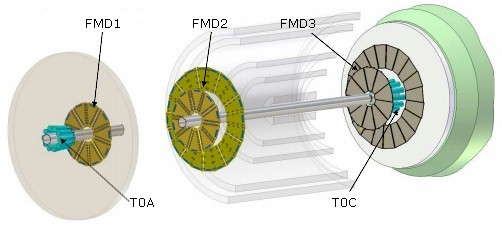
\includegraphics[scale=0.50]{figures/FMD.jpg}
  \caption{FMD and T0 detectors.}
  \label{fig:FMD}
\end{figure}
%
The FMD provides information about the charged particle multiplicity in the pseudorapidity ranges -3.4 $\leq \eta \leq$ -1.7 and 1.7 $\leq \eta \leq$ 5.1. The measurement of charged particle multiplicity is important to study the particle flows and event-by-event multiplicity fluctuations. The FMD is composed of five rings of silicon strip detectors, organized in three components: FMD2 and FMD3 consist of two rings, while FMD1 is made of just one ring. FMD3 is installed on the muon absorber side, FMD1 and FMD2 on the opposite side of the interaction point. FMD2 and FMD3 are placed at about 70 cm from the nominal interaction point, while FMD1 is placed much further from the interaction point, at about 320 cm on the side opposite to the muon arm.
\subsection*{VZERO}
The V0 consists of two arrays of scintillator counters (VOA\footnote{A = ATLAS: it is on the side towards the ATLAS experiment} and VOC\footnote{C = CMS: it is on the side towards the CMS experiment}). The V0A is located 340 cm from the nominal interaction point, on the opposite side to the muon spectrometer, and covers the pseudorapidity range 2.8 < $\eta$ < 5.1. The V0C, instead, is fixed to the front of the hadronic absorber, at 90 cm from the interaction point, and covers the pseudorapidity range -3.7 < $\eta$ < -1.7. Both the detectors cover the full azimuthal angle interval. The V0 has many functions: it provides the \textit{Minimum-Bias} triggers and centrality triggers for Pb-Pb events, it can be used to measure the event multiplicity at forward rapidity, from which the centrality of the event can be determined, it is used for the rejection of background events.
\subsection*{TZERO}
The detector consists of two arrays (T0A and T0C) of Cherenkov counters, placed at -72.5 cm and 375 cm from the interaction point. It covers the pseudorapidity ranges -3.28 < $\eta$ < -2.97 and 4.61 < $\eta$ < 4.92. Its main purpose is the generation of a start time (T0) for the TOF detector, but it can also be used for an independent determination of the vertex position along the beam line, with a precision of 1.5 cm, and to provide the first level (L0) trigger when the position is within the expected value.
\section{Trigger System and Data acquisition}
The trigger system in ALICE is handled by the \textit{Central Trigger Processor} (CTP), which receives trigger inputs from the triggers detectors and sends trigger signals to the readout detectors in case the trigger conditions are fulfilled. It is based on three level of hardware triggers (L0, L1 and L2) and a fourth level (\textit{High Level Trigger}) of software triggers. This multi-level trigger is needed because of the large differences in the readout time of the detectors.\\
Trigger classes (minimum bias, high multiplicity, dimuons) are the combination of the trigger inputs of different trigger detectors, obtained through logical operations with signals. The three trigger levels are characterized by a different response time. The L0 is a fast trigger, with a response time of 1.2 $\mu$s, and uses only detectors characterized by a high readiness, such as SPD\footnote{subdetectors of the ITS, described later}, T0 and V0. If the L0 conditions are matched, the CTP sends the trigger signal to the readout detectors, which start registering the event. The L1 has a response of 6.5 $\mu$s and involves signals from all the detectors: in case after the response time no signal has been received by the CTP, readout detectors stop registering the event. The L2 trigger is the final preliminary check before the data transfer. It looks for specific problems which can spoil, or even make impossible, the reconstruction of the event, like for example the presence of two sequential lead-lead collisions, which would cause a too high occupancy in the TPC. If the L2 requirements are fulfilled, the event can be sent to the \textit{Data AcQuisition System} (DAQ), which manages the data flow from the detectors to the archiving on tape. This process takes place in few steps. First, when the readout electronics of a detector is triggered, it sends data to a farm of 300 individual computers (\textit{Local Data Concentrators}) in the experimental site. Each LDC combines the fragment of data coming from detectors in sub-events. The sub-events are transferred to 40 \textit{Global Data Collectors}, computers that perform the event building. Each GDC is able to process up to 40 events in parallel. At this moment, the data rate coming from the different sub-detectors is about 25 GB/s and the size of a central data can be $\sim$ 70 MB. For this reason the High Level Trigger performs an additional event selection and compression, optimizing the use of recording band available. This data compression allows to reach a data rate of about 1.25 GB/s. Finally, event selected by the HLT are transferred to the CERN computer centre to be recorded on tape.
\section{ALICE Software}
\label{datavol}
The ALICE experiment software is based on ROOT \cite{ROOT}, the data analysis framework developed at CERN. ROOT is an object oriented framework, developed in C++ and characterized by a high flexibility that can be used in many different fields, even if its main applications are in particle physics. A dedicated group at CERN develops and maintains ROOT but many contributions come from the whole particle physicist community, being ROOT an open source project. This framework provides I/O handling functionalities and many advanced statistical tools.\\
The framework adopted by the ALICE offline project is AliRoot \cite{AliRoot}, an object oriented code based on ROOT. The main purpose of AliRoot is to provide a set of software classes and macros to reconstruct and analyse data coming from the ALICE apparatus. For this reason it includes the geometry of the ALICE detectors, their typology and their response to the passage of particles. In addition AliRoot provides the tools for the local reconstruction and analysis of each detector.\\
\begin{figure}
  \centering
  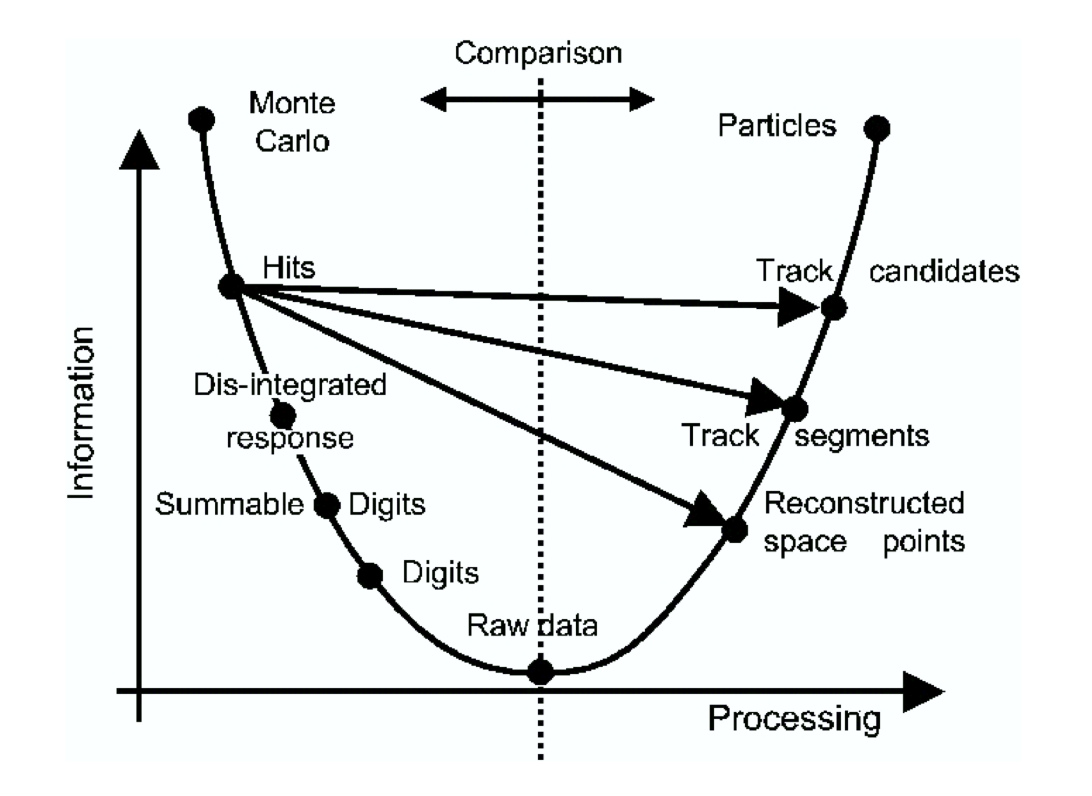
\includegraphics[scale=0.30]{figures/reconstruction.png}
  \caption{Simulation and reconstruction process.}
  \label{fig:Rec}
\end{figure}
%
A scheme of the work flow of the simulation and reconstruction process in AliRoot can be found in Figure \ref{fig:Rec}: the left part shows the simulation steps, followed in the Monte Carlo simulations, while the right part shows the reconstruction steps, common for both real and simulated data.\\
The particles produced in the collision are created using generator codes for heavy-ion interactions such as HIJING \cite{hijing} and PYTHIA \cite{pythia}. The generated particles are  then transported through the detector with transport codes like GEANT3/4 \cite{geant} and FLUKA \cite{fluka}, simulating the interaction with the material and the energy deposit in the active areas of the detectors, which constitutes the particle \textit{hits}. The hit keeps the information about the particle that generated it in form of a \textit{track label}. The next step is the simulation of the response to the hits of the detectors and the readout electronics. The digitization is done in two steps: \textit{summable digits}, produced with low thresholds and used for the \textit{event merging}, in which signals coming from different events are summed together; \textit{digits}, generated with real trigger thresholds after the noise simulation and comparable to real raw data.\\
During the reconstruction, digits are extracted from raw data and the adjacent digits are grouped together to form  a \textit{cluster}, which is the signal given by a particle in the detector. \textit{Rec-points} are defined by the reconstructed space position and, where possible, energy deposit. In the next step, the \textit{tracking}, the rec-points generated in the local reconstruction of each sub-detector are associated into \textit{tracks}, which contain the information about the kinematic parameters and the identity of the particles. Finally, the results from the reconstruction step are stored in \textit{Event Summary Data} (ESD, which can be further condensed into an \textit{Analysis Object Data} (AOD), containing the essential information needed for the analysis.
\section{Inner Tracking System}
\label{sec:ITS}
\begin{figure}
  \centering
  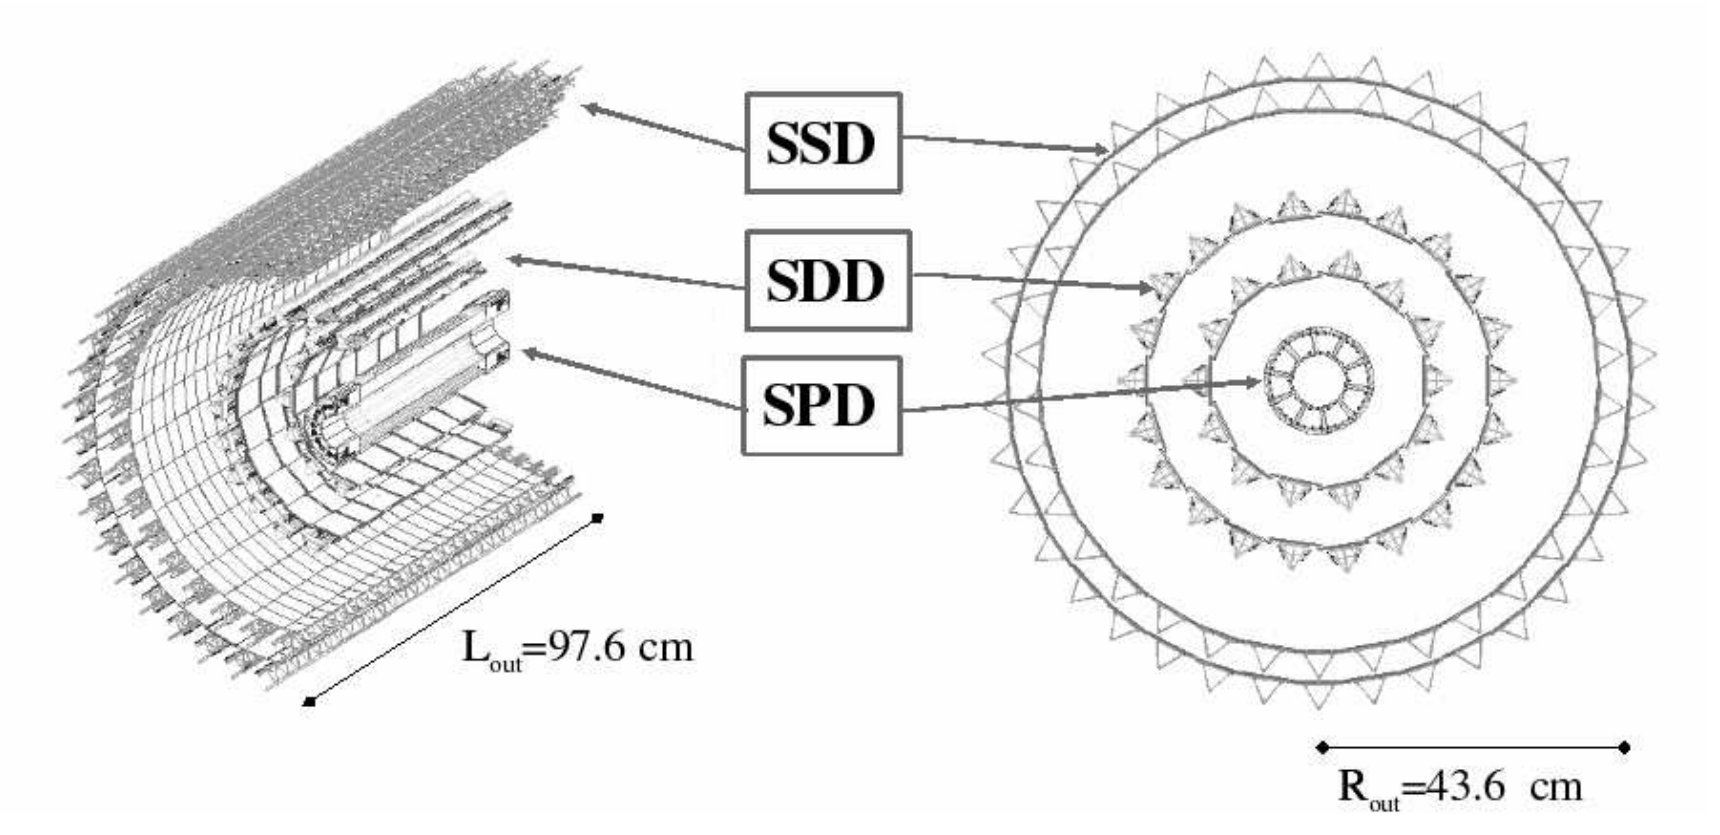
\includegraphics[scale=0.30]{figures/ITS.png}
  \caption{Layout of the ITS.}
  \label{fig:ITS}
\end{figure}
%
The ITS is the closest detector to the interaction point and it consists of six cylindrical layers of silicon detectors of different technologies: the two innermost layers are made of \textit{silicon pixel detectors} (SPD), the two central layers are made of \textit{silicon drift detectors} (SDD) and the two outer layers are made of double-sided \textit{silicon strip detectors} (SSD). The layout of the ITS is schematically shown in Figure \ref{fig:ITS}.\\
The ITS has a full acceptance in the azimuthal angle (2$\pi$) and it covers the pseudorapidity range of |$\eta$| < 0.9 (the same of the TPC) for all the collisions inside the so called \textit{interaction diamond}, the region in which |z| < 5.3 cm. The geometry of the ITS, i.e. the number, the position and the segmentation of the layers, has been optimized for the tracking efficiency and for a high resolution on the impact parameter, which in a decay is defined as the transverse distance of closest approach between a particle trajectory and the primary vertex (an example of impact parameter is shown in Figure \ref{fig:parametro}). The SPD covers a larger pseudorapidity, |$\eta$| < 1.2 for particles generated at z = 0, to provide, together with the FMD, continuous coverage for the measurement of charged particle multiplicity.\\
\begin{figure}
  \centering
  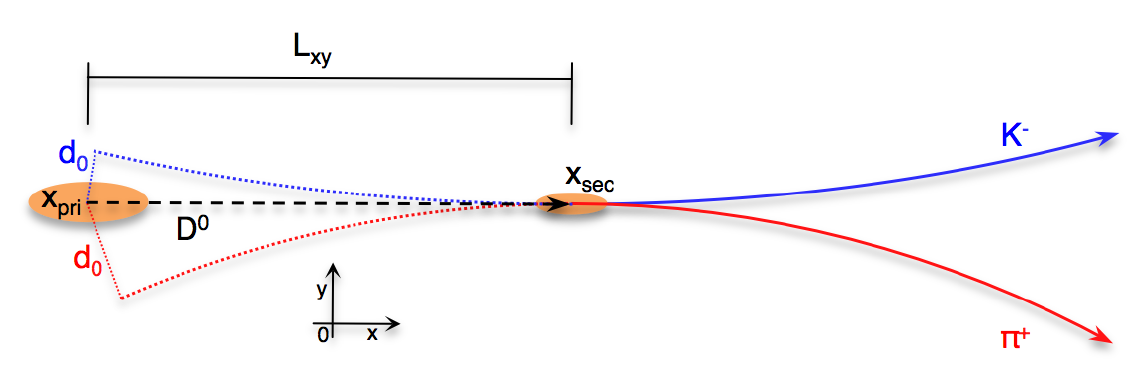
\includegraphics[scale=0.40]{figures/parametro.png}
  \caption{Example of impact parameters in the D$_0$ decay in the transverse plane.}
  \label{fig:parametro}
\end{figure}
%
\begin{table}
\centering
\renewcommand\arraystretch{1.5}
 \begin{tabular}{|c|c|c|c|c|c|}
  \hline
  Layer & Type & r (cm) & $\pm$z (cm) & $\#$ Modules & Material budget ($\%$ of X$_0$)\\
  \hline
  1 & pixel & 3.9 & 14.1 & 80 & 1.14 \\
  2 & pixel & 7.6 & 14.1 & 160 & 1.14 \\
  3 & drift & 15.0 & 22.2 & 84 & 1.13 \\
  4 & drift & 23.9 & 29.7 & 176 & 1.26 \\
  5 & strip & 38.0 & 43.1 & 748 & 0.83 \\
  6 & strip & 43.0 & 48.9 & 950 & 0.86 \\
  \hline
 \end{tabular}
 \caption{ITS geometrical and composition details.}
 \label{tab:ITSgeom}
\end{table}
%
\begin{table}
\centering
\renewcommand\arraystretch{1.5}
 \begin{tabular}{|l|c|c|c|}
  \hline
  Parameter & SPD & SDD & SSD \\
  \hline
  Spacial resolution in $r\varphi$ ($\mu$m) & 12 & 35 & 20 \\
  Spacial resolution in z ($\mu$m) & 100 & 25 & 830 \\
  Two tracks resolution in $r\varphi$ ($\mu$m) & 100 & 200 & 300 \\
  Two tracks resolution in z ($\mu$m) & 850 & 600 & 2400 \\
  Cell size ($\mu$m$^2$) & 50 $\times$ 425 & 202 $\times$ 294 & 95 $\times$ 40000 \\
  Active area per module (mm$^2$) & 12.8 $\times$ 69.6 &  72.5 $\times$ 75.3 &  73 $\times$ 40 \\
  Readout channel per module & 40960 & 2 $\times$ 256 & 2 $\times$ 768 \\
  Total number of modules & 240 & 260 & 1698 \\
  Total number of readout channels (k) & 9835 & 133 & 2608 \\
  Total number of cells (M) & 9.84 & 23 & 2.6 \\
  Max. occupancy (inner layer) (\%) & 2.1 & 2.5 & 4 \\
  Max. occupancy (outer layer) (\%) & 0.6 & 1.0 & 3.3 \\
  \hline
 \end{tabular}
 \caption{Parameters of the various detectors. The maximum occupancy is referred to the most central Pb-Pb collisions. In the ITS a module consists of a sensor element equipped with its front end electronics.}
 \label{tab:ITSparam}
\end{table}
%
The geometrical dimensions and the technologies used in the layers can be found in Table \ref{tab:ITSgeom}, while a list or the ITS characteristics can be found in Table \ref{tab:ITSparam}.\\
The SPD for the two inner layers as well as the SDD for the two middle ones have been chosen because of the high particle density expected in heavy-ion collisions at LHC (about 50 particles for cm$^2$ predicted for the innermost layer) and in order to achieve the needed impact parameter resolution.\\
The four outer layers (SDD and SSD) have an analogue  readout of the charge deposition and therefore can be used for the PID through the measurement of the $dE/dx$ in the non relativistic region of the Bethe-Bloch curve, where $dE/dx \propto 1/\beta^{2}$. For this reason the analogue readout has a large dynamic range to provide the $dE/dx$ for low-momentum particle, which are heavily ionising. This characteristic makes the ITS stand-alone a low-$\pt$ particle spectrometer.\\
Since for low momentum particles the multiple scattering can easily spoil the impact parameter resolution, the material budget of the ITS has been kept to a minimum. For the SDD and the SSD, which are also used to measure the energy deposit, have a minimum thickness of 300 $\mu$m to provide an acceptable signal-to-noise ratio. Also the additional material, such as electronics, cabling, supporting structures has been kept at comparable levels, so that a particle that passes through the whole ITS perpendicularly would traverse $\sim$ 8\% of a radiation length.\\
The ITS design has been optimized to keep good tracking efficiency in a high multiplicity environment, as expected in Pb-Pb collisions at the nominal energy of the LHC. For this reason the granularity of the detector has to be sufficiently high to guarantee a low occupancy, at the level of few  per cent. To achieve this requirement, several millions of active cells in each layer of the ITS are needed, as it can be seen in Table \ref{tab:ITSparam}. The highest granularity is reached in the two innermost layers with SPD,  but a good granularity is reached in the middle layers with SDD too. In the last two layers with SSD the track density is lower and therefore the granularity is lower too.\\
The spatial resolution needed is set by the $c\tau$ of the D mesons, which is of the order of 100 $\mu$m. The ITS has therefore been built with an impact parameter resolution better than 100 $\mu$m in r$\varphi$ plane and a of few tens of mm in z. Moreover, for momenta larger than 3 GeV/c the spatial precision of the ITS is an essential element of the momentum resolution.
\begin{figure}
  \centering
  \subfloat[][]
  {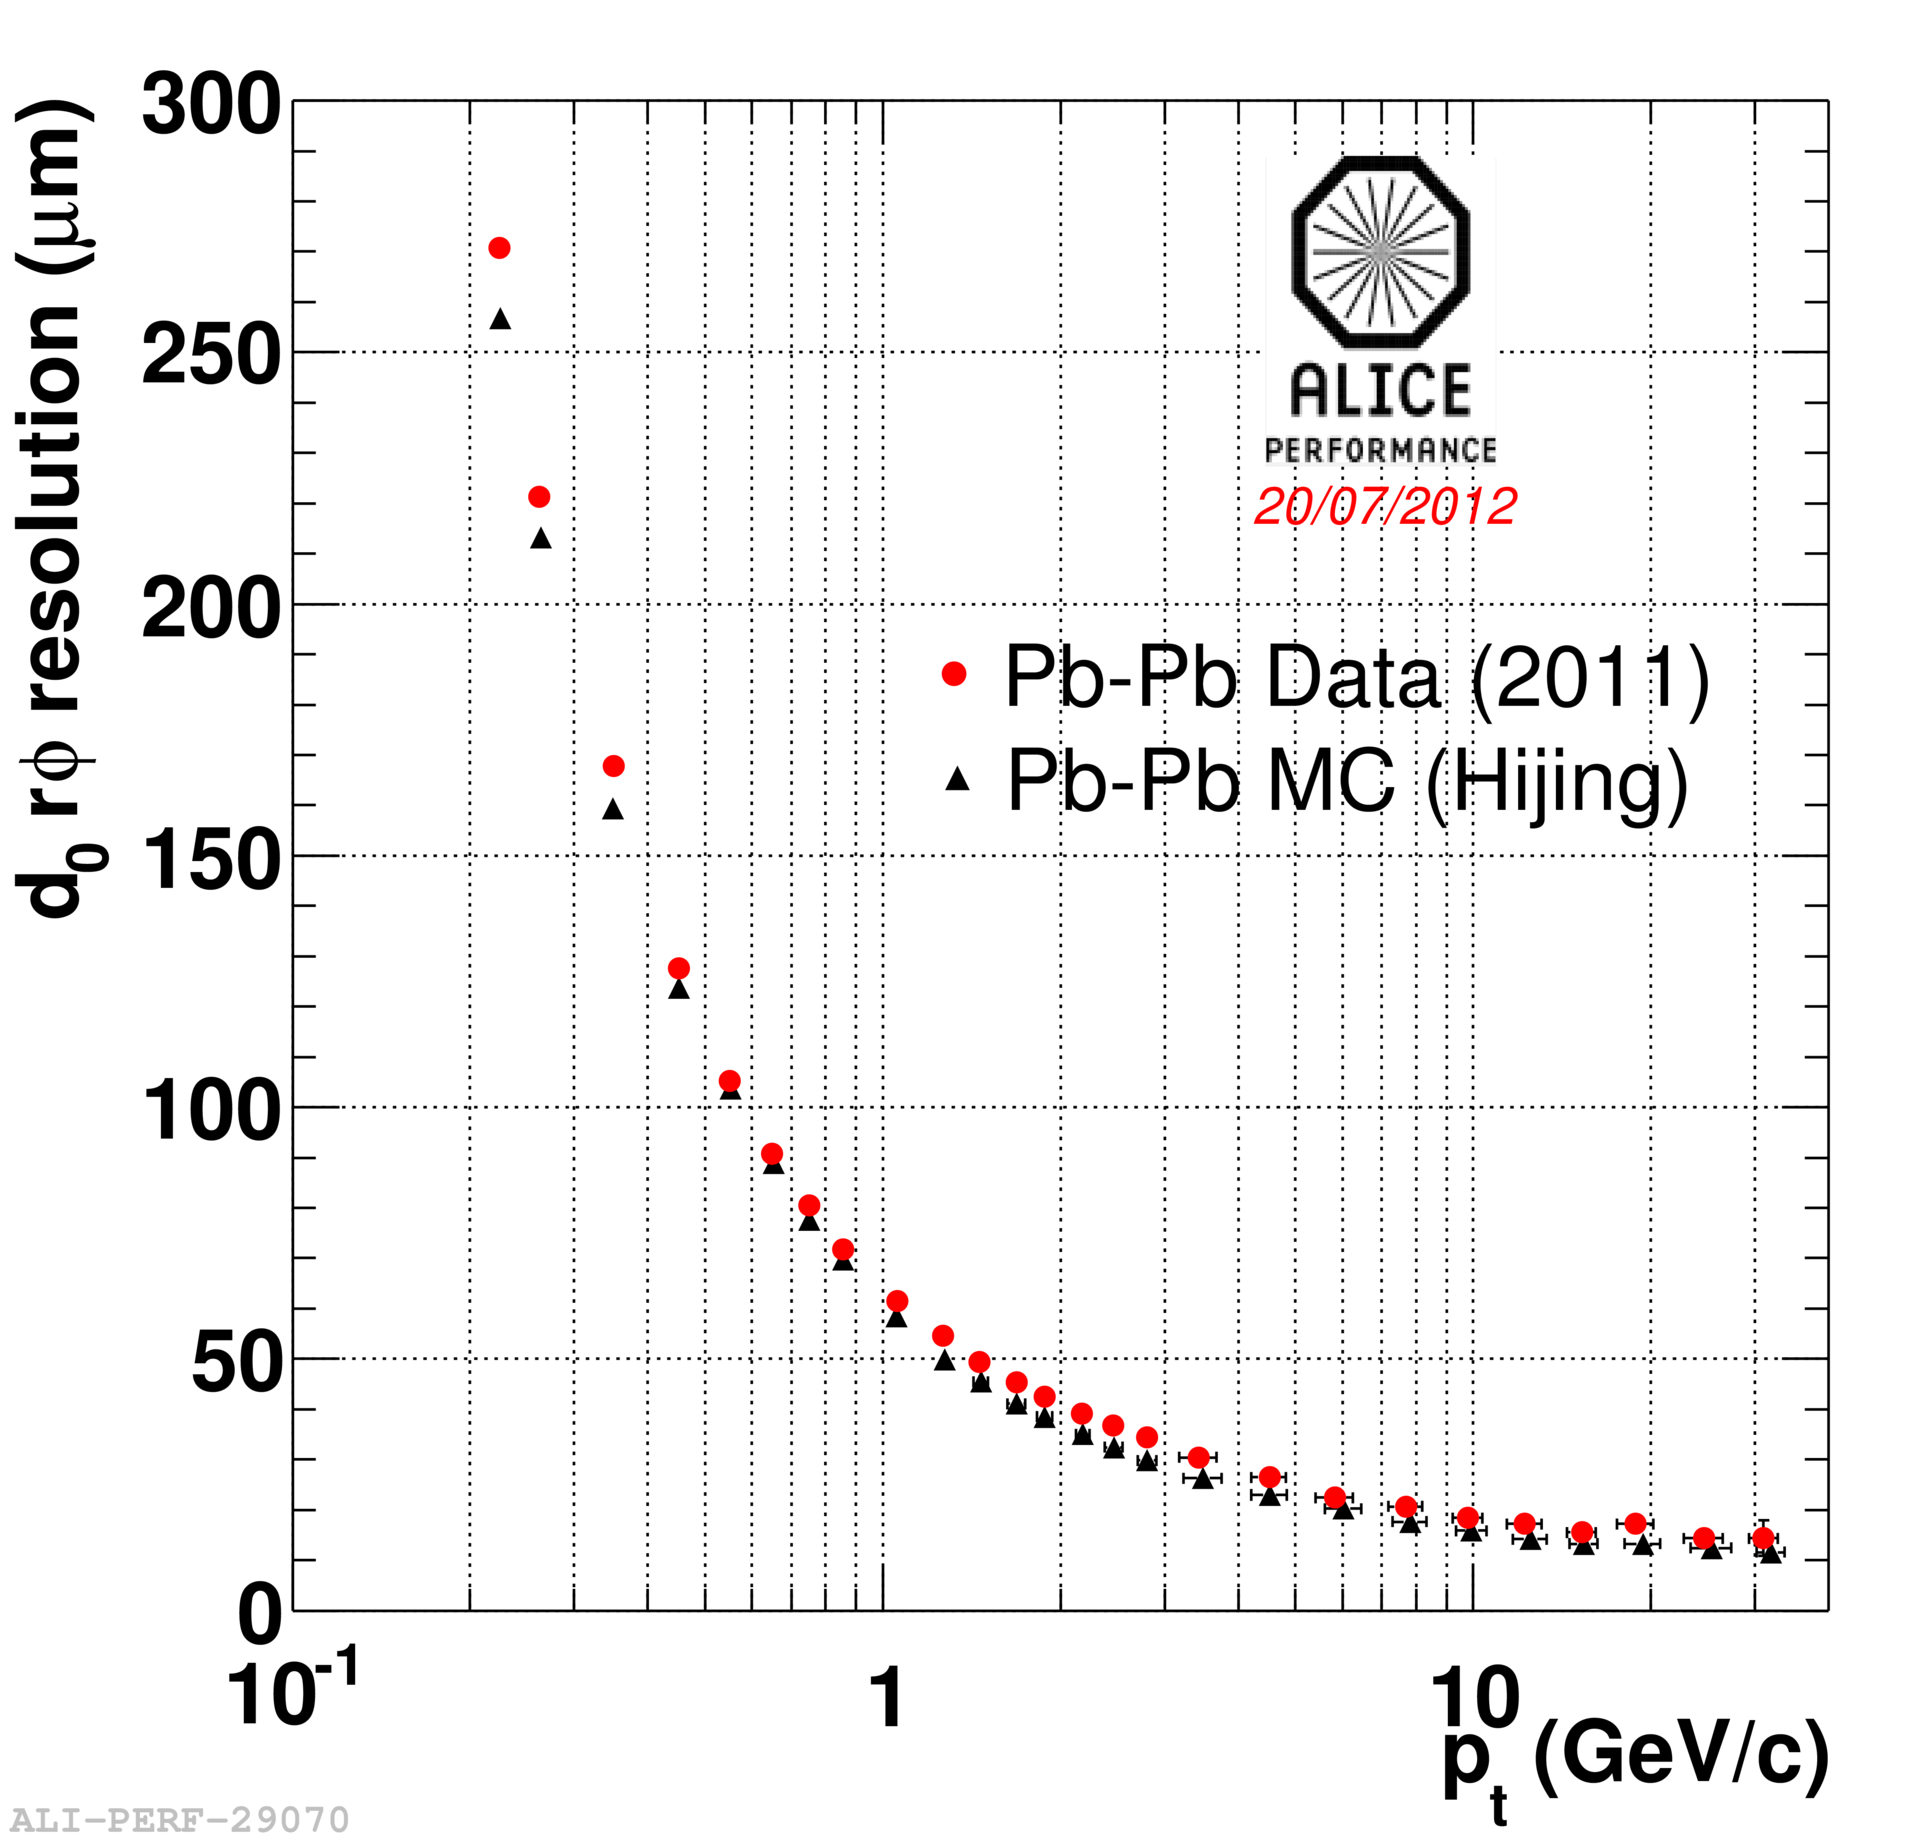
\includegraphics[scale=0.10]{figures/d0rphi.png}\label{fig:d0rphi}}\quad
  \subfloat[][]
  {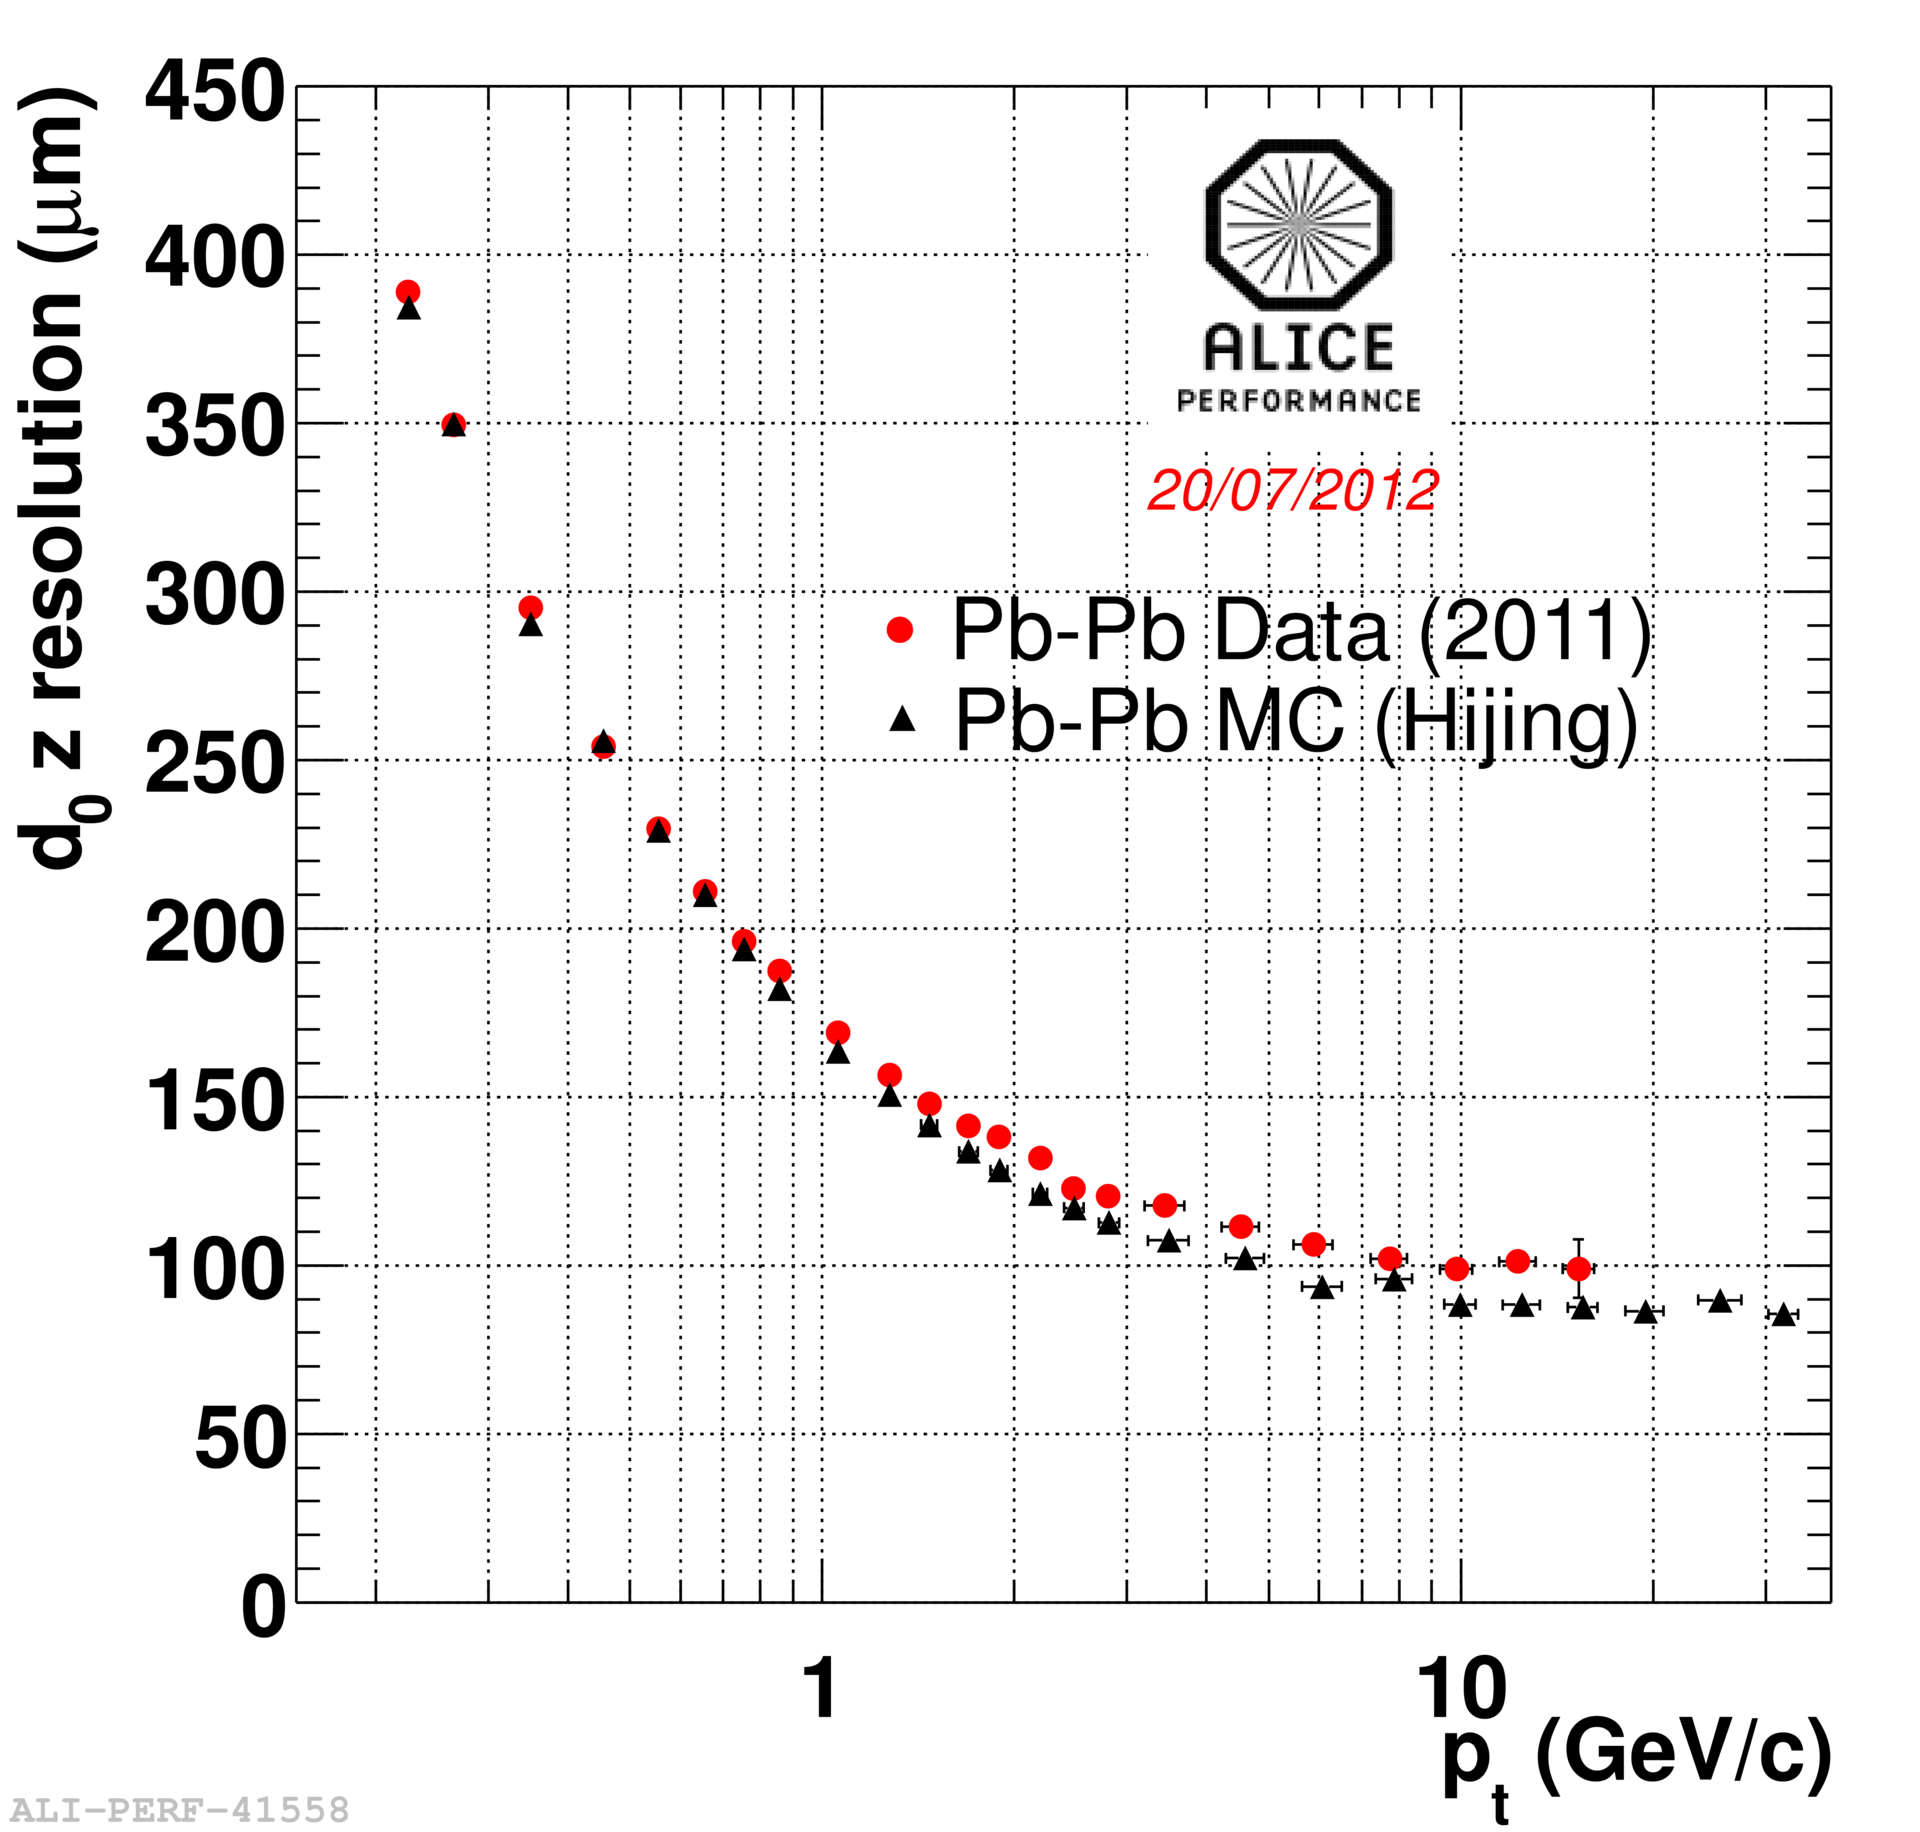
\includegraphics[scale=0.10]{figures/d0z.png}\label{fig:d0z}}
  \caption{Track impact parameter resolution in the transverse plane (a) and in the beam direction (b) in Pb-Pb 2011.}
\end{figure}
The impact parameter resolution as a function of the transverse momentum in r$\varphi$ and z can be seen in Figure \ref{fig:d0rphi} and \ref{fig:d0z}. In both the directions the resolution increases when the transverse momentum of the particle increases, reaching a value better than 20 $\mu$m and 100 $\mu$m in r$\varphi$ and z respectively for $\pt$ values larger than 10 GeV/c.\\
In the next sections the different detectors of the ITS will be described.
\section{Silicon Pixel Detector}
The role of the two innermost layers of SPD is crucial for the determination of the position of the primary vertex as well as for the measurement of the impact parameters of secondary particles originating from the weak decays of particles. The use of a truly two-dimensional detectors brings some advantages. First, the two-dimensional segmentation of the pixel detectors avoids the ghost hits that typically affect the double-sided strip detectors giving an ambiguous information about the hit points. Then, the small dimension of the single pixel (50 $\times$ 425 $\mu$m$^2$) gives a high spatial resolution, combined with a low diode capacitance, which implies an excellent signal-to-noise ratio.\\
The SPD is characterized by a binary digital readout: in each cell, a threshold is applied to the pre-amplified and shaped signal and the digital output level changes when the signal is above threshold. The threshold is about 100 electrons per cell.\\
It is divided in modules, which consist of a two-dimensional matrix of silicon pixel detectors, also called sensor ladder, bounded to the related front-end electronics. Each matrix is made of 256 (r$\varphi$) $\times$ 160 (z) pixels, with a total area of 12.8 mm (r$\varphi$) $\times$ 69.6 mm (z). Two modules aligned in z direction form a \textit{half-stave}, whose length is 141.6 mm. Two half-staves are attached head-to-head laong the z direction to a carbon fibre support sector to form a stave. Each sector supports six staves and provides the cooling for the detectors.\\

\section{Silicon Drift Detector}
\begin{figure}
  \centering
  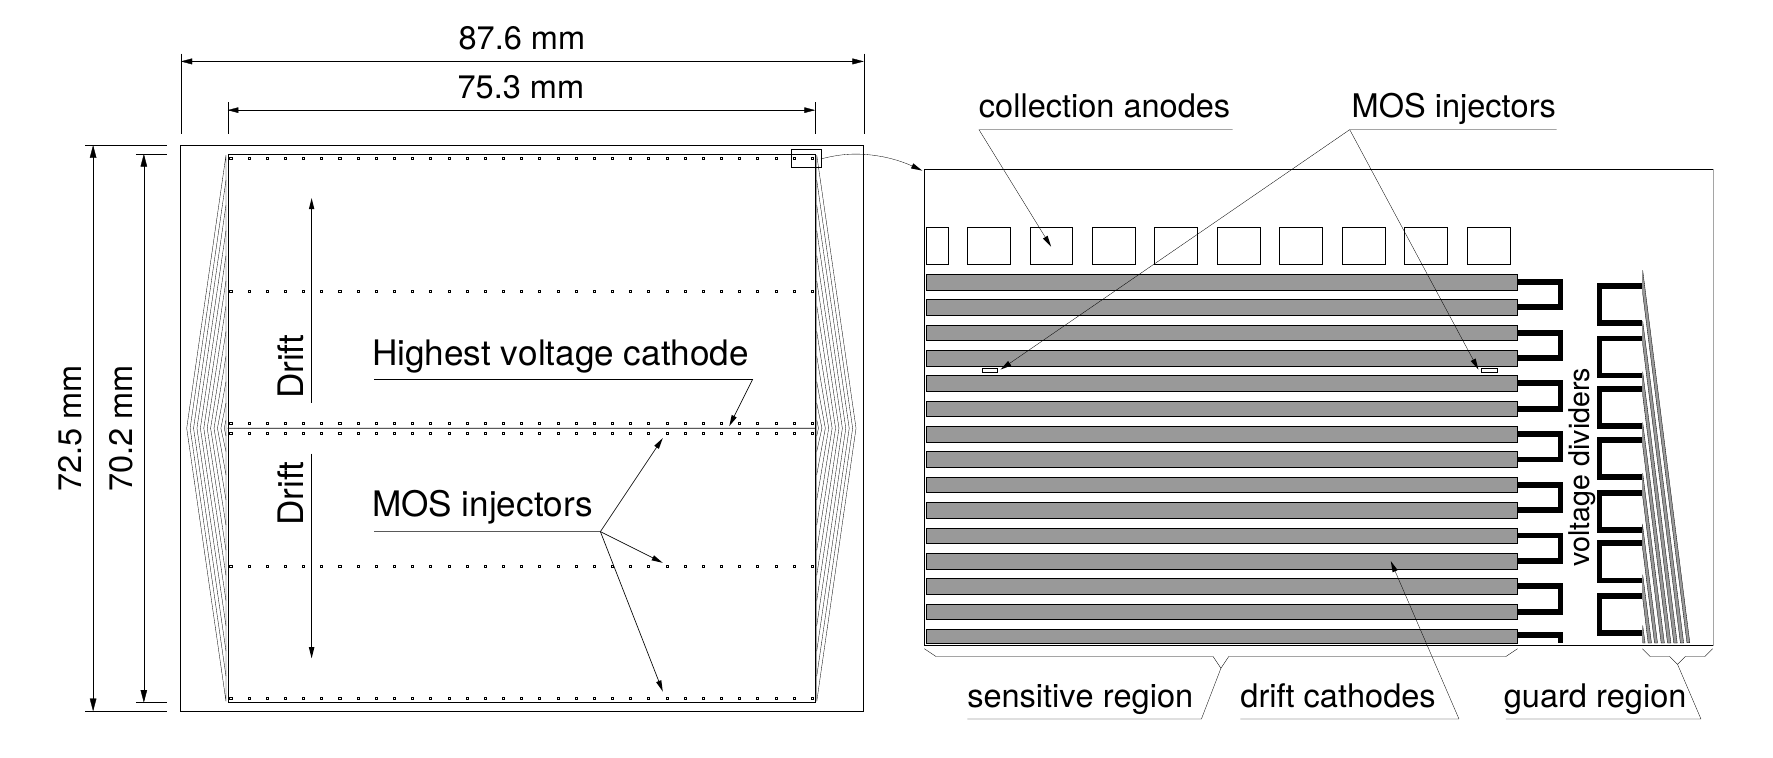
\includegraphics[scale=0.30]{figures/SDD.png}
  \caption{Layout of the ALICE SDD.}
  \label{fig:SDD}
\end{figure}
%
\begin{figure}
  \centering
  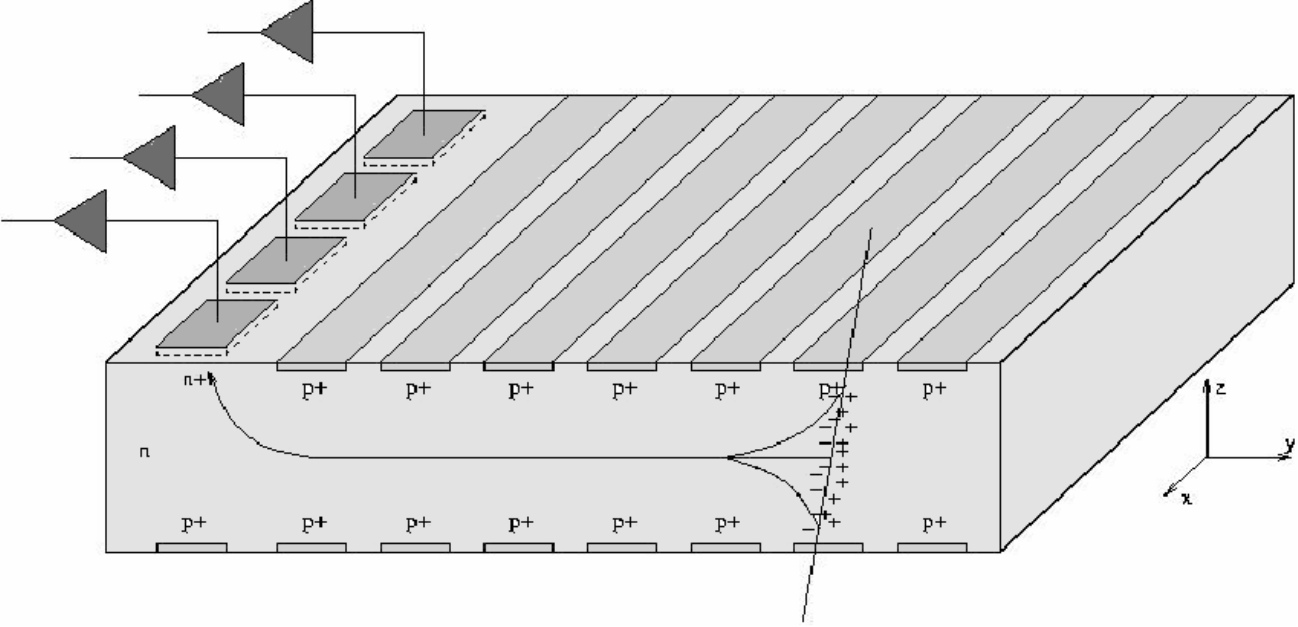
\includegraphics[scale=0.25]{figures/sddw.png}
  \caption{Representation of the working principle of the SDD.}
  \label{fig:sddw}
\end{figure}
%
The SDD constitutes the two intermediate layers of the ITS and is located in a region where the charged particle density is lower than for the SPD. The layout of a SDD sensor can bee seen in Figure \ref{fig:SDD}. The single drift detector gives a two-dimensional information about the position of the particle. The z-coordinate of the impact point can be determined by the centroid of the charge collected by the anodes. The position along the r$\varphi$ direction, instead, is obtained measuring the time necessary to the electrons produced by the ionizing particle crossing the detector to drift to the collecting anodes under the effect of an electric field. This is possible thanks to the constant drift velocity during the data acquisition. The drift time is measured with respect to the trigger time. A representation of the working principle of the SDD can be found in Figure \ref{fig:sddw}.\\
The SDDs are produced from 300 $\mu$m thick silicon wafers, characterized by a high resistivity (3 k$\Omega$cm) and a good doping homogeneity (5\%). They have a sensitive area of 70.17 (r$\varphi$) $\times$ 75.26 (z) mm$^2$ and a total area of 72.50 (r$\varphi$) $\times$ 87.59 (z) mm$^2$. The sensitive area is split into two drift regions by a central cathode strip, with a high voltage bias of -1.8 kV. On each surface of the drift region, 291 p$^+$ cathode strips, with 120 $\mu$m pitch, fully deplete the detector volume and generate a drift field parallel to the surface. The drift field is obtained with a voltage divider located on the detector sides, which scales down the HV applied from the central cathode towards the anodes. Each drift region contains 256 collection anodes with 29 $\mu$m pitch and 33 MOS charge injectors to monitor the drift velocity and, therefore, calibrate the sensor. The drift velocity is dependent on the temperature (v$_{drift} \propto$ T$^{-2.4}$) and for this reason the temperature fluctuations must be limited ($\Delta$T $\leq$ 0.1 K). For a HV of -1.8 kV applied to the central cathode, the drift velocity is 6.5 $\mu$m/ns. Since the front-end electronics samples the signal for each anode with a rate of 40 MHz, the size of a cell is 294 $\times$ 202 $\mu$m$^2$, corresponding to about 9000 cells for sensor, which are readout by 512 electronics channels. Therefore SDD are characterized by a good 2D resolution with a low number of readout channels.\\
Moreover, since the collective charge is proportional to the energy loss of the particle within the sensor, SDDs can also be used for particle identification via \textit{dE/dx}, thanks to the presence of the analogue readout electronics.\\
The signal readout of the SDD is based on three stages. The first, the PASCAL chip, consists of a preamplifier, an analogue storage and an analogue-to-digital converter (DAC) and works at a frequency of 20 MHz. The second stage is AMBRA, which is a digital four-event buffer which performs the baseline equalization on anode-by-anode basis and the 10-bit to 8-bit non-linear data compression. The final stage is CARLOS, which performs the zero-suppression and the data compression. It is very important to underline that the passage of information fron AMBRA to CARLOS take 1.23 ms, but reduce the SDD event size by more than an order of magnitude.\\
Finally, a SDD module consists of one silicon drift detector and two front-end chips. The modules are mounted on linear structures called ladders: there are 14 ladders with six modules each on the third layer and 22 ledders with eight modules each on the fourth layer. The ladders are assembled on a \textit{Carbon Fibre Reinforced Plastic} (CFRP) structure. 
\section{Silicon Strip Detector}
The two outer layers of the ITS are made of double-sided silicon strip detectors. In the ALICE tracking system, the SSD plays an extremely important role in the track propagation from the TPC to the ITS. In addition to the two-dimensional information on the particle position, it provides also information on the collected charge, thanks to the analogue readout electronics. Therefore in the SSD the \textit{dE/dx} information can be used for the particle identification in the low momentum region.\\
The sensors are 300 $\mu$m thick and they have 768 strips on each side, with a pitch of 95 $\mu$m and a length of 40 mm. Sensors are mounted with the strips nearly parallel to the magnetic field in order to optimize the resolution in the bending direction. Moreover, the sensor p-side (n-side) of layer 5 (layer 6) faces the interaction region, resulting in four almost equally spaced strip orientations in the two layers, which significantly reduces the number of ambiguities seen by the tracking software.\\
A SSD module consists of one sensor connected with two front-end electronic chips. The modules are assembled on ladders of the same design as those supporting the SDD. There are 748 ladders on the fifth layer and 960 on the sixth, for a total number of modules of 1698. The ladders are assembled on a \textit{Carbon Fibre Composite} support structure.\\
The electronic signals from the modules are AC-coupled and buffered in custom made electronics, the \textit{EndCap Modules} (ECM), located at each end of each ladder. The analogue-to-digital conversion of the signals is performed in the \textit{Front-End ReadOut Modules} (FEROM), located outside the ALICE magnet.
\chapter{The Upgrade of the ITS}
%\lettrine{D} {$\mkern-\thinmuskip$}
During its first years of activity, the ALICE experiment has observed the creation of hot hadronic matter at unprecedented values of temperature and density, confirming the nature of the QGP as an almost-perfect fluid, as shown in previous experiments at BNL RHIC. Thanks to its unique tracking and PID capabilities, the measurements of the ALICE experiments exceeded the precision and kinematic reach of the QGP measures of its predecessors. However, it is still necessary to carry out high precision measurements of rare probes over a wide $\pt$ range, for which the current setup is not optimised.\\
In 2020, during the third run of data acquisition (Run3), the LHC will increase the luminosity of Pb-Pb collisions, reaching the interaction rate of 50 kHz, corresponding to an instantaneous luminosity of 6$\mathrm{\times 10^{27} cm^{-2}s^{-1}}$. The current collision rate is 8 kHz, while the readout rate of the detectors of the central barrel of the ALICE experiment is  0.5 - 1 kHz. For this reason, the current experimental set up does not allow to analyse all the Pb-Pb collisions provided by the LHC. For Run3, instead, the ALICE experiment will be upgraded to enable the readout of heavy-ion collisions at the rate of 50 kHz. Indeed, it is necessary to collect the data corresponding to all the Pb-Pb events, since for the objectives of the experiment no triggers are available. After the upgrade, more than 10 $\mathrm{nb^{-1}}$ of Pb-Pb collisions will be collected \cite{uptdr}. Among the detectors of the ALICE experiment, the Inner Tracking System will be replaced with a new detector. In this chapter, the upgraded ITS will be described, focusing on the physics motivations behind the upgrade, the layout of the new detector and the plans for the software development.
\section{Physics Motivations for the Upgrade}
One of the objectives of the upgrade is the study of heavy flavours, which are extremely important in heavy-ion physics since they are mainly produced in the first stages of the collision and, therefore, they allow to study the transport properties of the medium. There are two main questions related to the heavy-flavour interactions in the QGP:
\begin{itemize}
 \item the thermalization of heavy quarks in the medium, studying the baryon/ meson ratio for charm ($\Lambda_{c}$/D) and for beauty ($\Lambda_{b}$/B), the azimuthal anisotropy $v_2$ for charm mesons and baryons and possible in-medium thermal production of charm quarks.
 \item the heavy-quark in-medium energy loss and its mass dependence, which can be studied by measuring the nuclear modification factors $\RAA$ of $\pt$ distributions of D and B in a wide momentum range.
\end{itemize}
For all these measurements, it is necessary to reconstruct the open charm and beauty down to low transverse momentum ($\pt \leq$ 1 GeV/c) and to collect large statistics. The current configuration is not sufficient to fulfill these requests and an upgrade of the experimental setup is necessary. In particular, a larger statistics can be collected thanks to the higher collision rate, while the enhancement of the tracking resolution at low $\pt$ can be achieved with a low material budget.\\
Thanks to the reduced material budget and to the improved tracking precision and efficiency, it is possible to carry out a detailed measurement of low-mass dielectrons. These measurements are important because they give access not only to the thermal radiation from the QGP, of both real and virtual photons, but also to the in-medium modification of hadronic spectra related to chiral-symmetry restoration \cite{chiral}. Indeed, lattice QCD predicts that, at high temperatures, the restoration of chiral symmetry occurs, bringing some distortions in the vector and axial current spectra. This can empirically be seen as a change in the mass spectra, in particular for the meson $\rho$ in it $e^+e^-$ decay mode. This measurement implies the electron detection down to $\sim$ 100 MeV/c and, since the production rates of the thermal dileptons are low, a very good electron identification is needed to suppress combinatorial background, constituted primarily from $\pi^0$ Dalitz decays and photon conversions. For this reason, the upgraded experimental apparatus must be characterized by a low material budget before the first active layer. Moreover, good low-$\pt$ tracking capabilities are needed to track electrons down to $\pt \gtrsim $ 50 MeV/c, improving the reconstruction efficiency for the background suppression. Finally, by improving the secondary vertex resolution, it will be possible to discern electrons from semileptonic charm decays and to separate the charm contribution, allowing a better measurement of the thermal radiation.\\
The strong PID capabilities of the ALICE experiment are suitable for the spectroscopy of hypernuclei and exotic objects produced in Pb-Pb collisions. Hypernuclei are nuclei that contain at least a strange baryon (hyperon) in addition to protons and neutrons and their lifetime depend on the strength of the hyperon-nucleon interaction. The importance of such interactions is not only to describe the hadronic phase of a heavy-ion collision, but also to describe the hadronic matter in extreme density conditions, as for instance in neutron stars. In this context hyperon interactions are crucial to understand the phase structure of QCD at large densities. In particular, the mesonic decays of $^{3}_{\Lambda}$H , $^{4}_{\Lambda}$H  and $^{4}_{\Lambda}$He  are studied. The current data allows the detection of these states, but with a poor significance. Therefore, to improve the heavy-nuclear state analyses, the ALICE upgrade must fulfill two requirements: first, it must provide a larger statistics; then, it must improve the separation of the reconstructed signal decays from the combinatorial background, which can be obtained enhancing the tracking resolution. Besides the hypernuclei, more exotic forms of deeply bound states with strangeness have been proposed as states of matter, either consisting of baryons or quarks. Among these exotic objects, there are the H dibaryons, bound states of two $\Lambda$ mesons, and $\Lambda n$ bound states. These states have not been observed yet and hence, if they exist, are extremely rare. Moreover, the topology of their decay is very complex, making the detection efficiency low. Similarly to the case of hypernuclei, this analysis would benefit from the larger statistics and from a better tracking resolution.
\section{Layout of the ITS-Upgrade}
The readout rate of the current ITS is a strong limit: the readout times and the corresponding rate capabilities of the sub-detectors of the current ITS are reported in Table \ref{tab:curr}. These times depend only marginally on the detector occupancy and are very similar for pp and Pb-Pb collisions. The maximum rate of the current ITS is therefore about 1 kHz, with 100\% dead time, and constitutes a strict limit for the future physics studies. Moreover, the current configuration of the ITS is not sufficient for the study of heavy flavours. Indeed, heavy flavours are characterized by a short proper decay length ($c\tau$) and these values are low if compared to the current impact parameter resolution. In particular, the most abundantly produced charm baryon, the $\Lambda_{c}$, has a proper decay length of 60 $\mu m$, which is below the impact parameter resolution of the present ITS (see Figure \ref{fig:d0rphi}) in the transverse momentum range of the majority of the $\Lambda_{c}$ daughter particles. For this reason, the physics of charm baryons, along with that of beauty mesons and of beauty baryons, in not accessible with the current detector.\\
%
\begin{table}
\centering
\renewcommand\arraystretch{1.5}
 \begin{tabular}{|c|c|c|}
  \hline
  Sub-detector & Readout time ($\mu s$) & Rate (Hz)\\
  \hline
  SPD & 296 & 3300 \\
  SDD & 1023 & 985 \\
  SSD & 310 & 3265 \\
  \hline
 \end{tabular}
 \caption{Readout time of the current ITS sub-detectors and maximum rate capability.}
 \label{tab:curr}
\end{table}
%
In Run3 the current limitations will be overtaken with the complete substitution of the ITS. The ITS-Upgrade (ITSU) will consists of seven layers of sensors, to be compared with the six layers of the current configuration. The insertion of a further layer, closer to the interaction point, is possible thanks to the reduction of the size of the beam-pipe. The number and the radial positions of the layers have been determined considering the available space from the beam-pipe to the outer layer of the current ITS and studying, using Monte Carlo simulations, the disposition that optimizes the $\pt$ resolution in stand-alone mode.\\

\noindent
The key features of the ITSU, compared with the characteristics of the current ITS, will be briefly described in the following.
\begin{itemize}
 \item \textbf{First layer closer to the interaction point.}\\
 The current beam-pipe, with a radius of 29 mm, will be replaced with a new beam-pipe, with a radius of 19.2 mm. The thickness of the beam-pipe will remain 0.8 mm. Thanks to this change, in the upgrade layout the first active layer of the detector, which is currently positioned at 39 mm from the beam line,  will be positioned at 22.4 mm for the beam-line.
 \item \textbf{Reduction of the material budget.}\\
 The reduction of the material budget in the ITSU, in particular of the first active layer, is a key point in the improvement of the impact parameter resolution, enhancing the tracking performances and the momentum resolution. The improvement in the tracking resolution with the reduction of the material budget can be explained considering the Coulombian multiple-scattering formula \cite{pdg}:
 \begin{equation*}
  \theta_0 \; = \; \frac{13.6}{\beta c p } \: z \:  \sqrt{\frac{x}{X_0}} \: \left[1 + 0.038\ln\left(\frac{x}{X_0}\right)\right]
 \end{equation*}
 where $\theta_0$ is the angular dispersion, $\beta c$ is the speed of the charged particle, $p$ its momentum, $z$ its charge (expressed in terms of the elementary charge $e$), $x$ the thickness of the material and $X_0$ its radiation length. It is therefore clear that reducing the thickness of the material, the effects of the multiple scattering become smaller, allowing a better reconstruction of the trajectory of the particle. The reduction of the material budget will be achieved using \textit{Monolithic Silicon Pixel Sensors} (MAPS), passing form 200 $\mu m$ of the current SPD to 50 $\mu m$. MAPS will be described more in detail later. Moreover, thanks to the optimisation of the readout chain, the power density is reduced of a factor of 2 if compared to the current sensors, allowing to increase the pixel density of a factor of 50. The lower consumption and the optimized power and signal distribution allow the reduction of the material budget of the electrical power and the signal cables. The final result is a detector with a thickness of 0.3\% $X_0$ for the three inner layers and of 0.8\%  $X_0$ for the outer layers.
 \item \textbf{Geometry and segmentation.}\\
 The ITSU will consist of seven layers of silicon pixels sensors. The three innermost layers form the \textit{Inner Barrel}, the remaining layers form the \textit{Outer Barrel}. The sensors of all the layers are segmented in pixels with dimensions of 20 $\times$ 20 $\mu m^2$. The layers are azimuthally segmented in units named \textit{Staves}, which are fixed to a support structure, half-wheel shaped, to form \textit{Half-Layers}. A single Stave consists of few elements:
 \begin{itemize}
  \item the \textit{Space Frame} is the mechanical support structure of the single stave, made of carbon fibre;
  \item the \textit{Cold Plate} is the carbon ply that embeds the cooling pipes;
  \item the \textit{Hybrid Integrated Circuit} is the flexible printed circuit (FPC) on which the Pixel Chips (two rows of seven sensors each) are bonded, along with passive components.
 \end{itemize}
 The Staves of the Outer Barrel are longitudinally segmented into \textit{Modules}, consisting of a Hybrid Integrated Circuit glued onto a carbon plate. Moreover, the Staves of the Outer Barrel are further segmented in azimuth in two halves, named \textit{Half-Staves}, which consist of a number of modules glued on a common cooling unit. The geometrical information about the ITSU is reported in Table \ref{tab:itsu}. 
 %
\begin{table}
\centering
\renewcommand\arraystretch{1.5}
 \begin{tabular}{|c|c|c|c|c|}
  \hline
  Layer & r (cm) & x/$X_0$ (\%) & \# sensors & \# staves\\
  \hline
  1 & 2.2 & 0.3 & 108 & 12\\
  2 & 3.0 & 0.3 & 144 & 16\\
  3 & 3.8 & 0.3 & 180 & 20\\
  4 & 19.4 & 0.8 & 2688 & 24\\
  5 & 24.4 & 0.8 & 3360 & 30\\
  6 & 34.2 & 0.8 & 8232 & 42\\
  7 & 39.2 & 0.8 & 9408 & 48\\
  \hline
 \end{tabular}
 \caption{Characteristics of the layers of the ITSU \cite{uptdr}.}
 \label{tab:itsu}
\end{table}
%
\begin{figure}
  \centering
  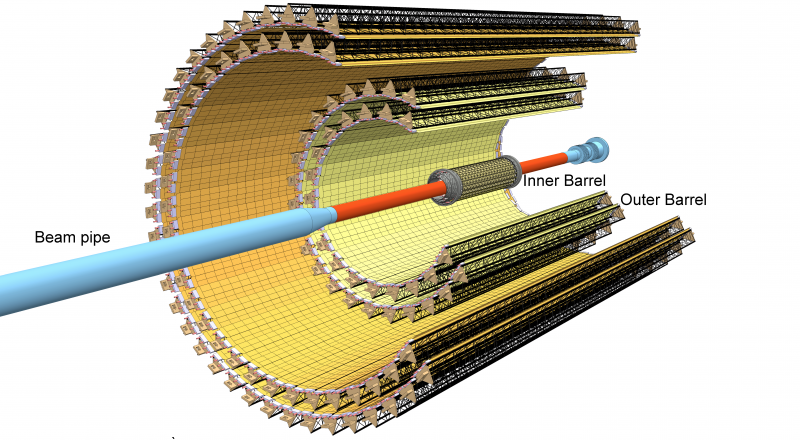
\includegraphics[scale=0.4]{figures/itsu.png}
  \caption{Layout of the upgraded Inner Tracking System.}
  \label{fig:build}
\end{figure}
%
\item \textbf{Binary readout}\\
In the ITSU there will be no analogue readout of the collected charge: each pixel has a single charge threshold and only the information whether a particle passed or not is available. Therefore, in the ITSU the particle identification via $dE/dx$ measurement will not be possible.
\item \textbf{Readout time}
The new detector is designed to be able to read data related to each individual interaction up to a rate of 100 kHz for Pb-Pb collisions and 400 kHz for pp collisions, a factor of 2 higher than the requirements. The new detector will support two different readout modes. 
In the \textit{continuous readout} mode, the information of the pixel matrices is shipped off-detector continuously, without a definition of event at readout level. The association of fired pixels to an event is done at the reconstruction level in the online system. In the \textit{trigger readout} mode, instead, only the fired pixels occurring in a particular time window that includes the event are shipped to the online system.
\end{itemize}
\section{MAPS}
\label{sec:maps}
Currently, the innermost layers of all the experiments of LHC are made of silicon pixel sensors bump-bonded on the readout electronics. Although this technology can be optimised, it has technical limitations that are close to be reached. For this reason, in the ITSU, Monolithic Active Pixel Sensors will be used: each pixel is monolithic, i.e. in the same piece of silicon both the active region and the readout electronics are present. In this way, it is possible to reduce the thickness of the sensors from the current value of 200 $\mu m$ for the SPD down to 50 $\mu m$. The working principle of a MAPS is shown in Figure \ref{fig:maps}. When a charge particle passes through the active volume of the silicon sensor, it liberates carriers in the semiconductor material. The released charge is collected by a sensing diode, which is a n-well normally used as a substrate of PMOS transistors. Consequently, only NMOS can be used in the pixel area, since a PMOS requires an additional n-well, which competes with the sensing diode in collecting the signal charge. Therefore, the front-end electronics fully relies on NMOS transistors and the n-wells that accommodate PMOS transistors are shielded by a deep p-well. Indeed, the deep p-well reflects the signal electrons so that they can be collected only by the sensing diode.
%
\begin{figure}
  \centering
  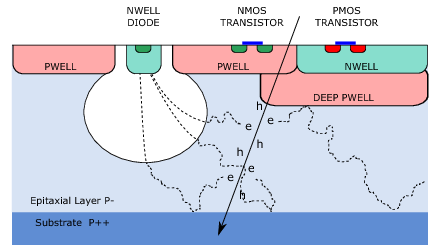
\includegraphics[scale=0.7]{figures/maps.png}
  \caption{Schematic cross section of a MAPS pixel \cite{uptdr}.}
  \label{fig:maps}
\end{figure}
%
The sensors must fulfill few requirements. First of all, they must have a low material budget and this condition is satisfied. Then, the performances of the ITSU and in particular its capabilities of separating secondary vertices of heavy-flavour decays are determined by the impact parameter resolution, which is enhanced thanks to the fine segmentation. Other important parameters for the track reconstruction are the detection efficiency, which must be at least 99\%, and the fake hit rate, which must be no more than $10^{-5}$. The performances of the sensors will be analysed later in this chapter.\\
Several prototypes of MAPS have been studied in the last years and the chosen one is ALPIDE (\textit{ALICE PIxel DEtector}), which is currently under development. This sensor has an active area of $15\times30 $ $mm^2$, corresponding to $512 \times 1024$ pixels with an extension of $20\times20$ $\mu m^2$ each. ALPIDE is characterized by a high-resistivity epitaxial layer (> 1 k$\Omega$), that allows a good charge collection. Its binary readout is performed with a combination of in-pixel discriminating frontend with a hit-driven combinatorial circuit. The former consists of a continuously active discriminating amplifier and a multiple-event memory in which the pixel information is stored. The memory is read out using a priority encoder, which takes into account only fired pixels: thanks to the low expected occupancy, the operation of pixel readout is fast \cite{alpide}.
\section{Detector Performances}
In this section the performances of the ITSU will be described. The results have been obtained using Monte Carlo simulations, with the geometrical parameters of the detectors previously described. The particle pseudorapidity-density has been extrapolated by the multiplicity measurements of Pb-Pb collision at $\sqrt{s_{NN}}$ = 2.76 TeV, obtaining a value of $dN_{ch}/d\eta \approx$ 1970 for central Pb-Pb collisions at $\sqrt{s_{NN}}$ = 5.5 TeV.
%
\begin{figure}
  \centering
  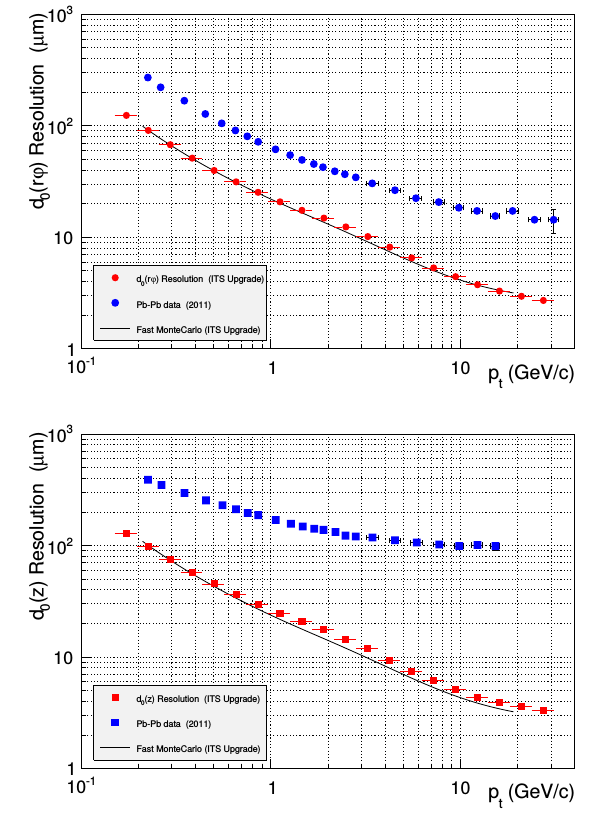
\includegraphics[scale=0.6]{figures/impactsim.png}
  \caption{Impact-parameter resolution for primary charged pions for the current ITS and for the ITSU in $r\varphi$ direction (upper panel) and $z$ direction (lower panel)\cite{uptdr}.}
  \label{fig:impactsim}
\end{figure}
%
The first important parameter is the impact-parameter resolution, since it defines the detector capability to discern the secondary vertex of heavy flavours from the primary vertex. This quantity is defined as the width of the distribution of the distances of closest approach between the reconstructed track and the interaction point. In Figure \ref{fig:impactsim} a simulation of the impact-parameter resolution for primary pions is shown together with the resolution in Pb-Pb data of the current detector. It is possible to see how the resolution will improve of a factor of 3 for $\pt$ < 1 GeV/c and of a factor of 5 for $\pt$ > 10 GeV/c.\\
%
\begin{figure}
  \centering
  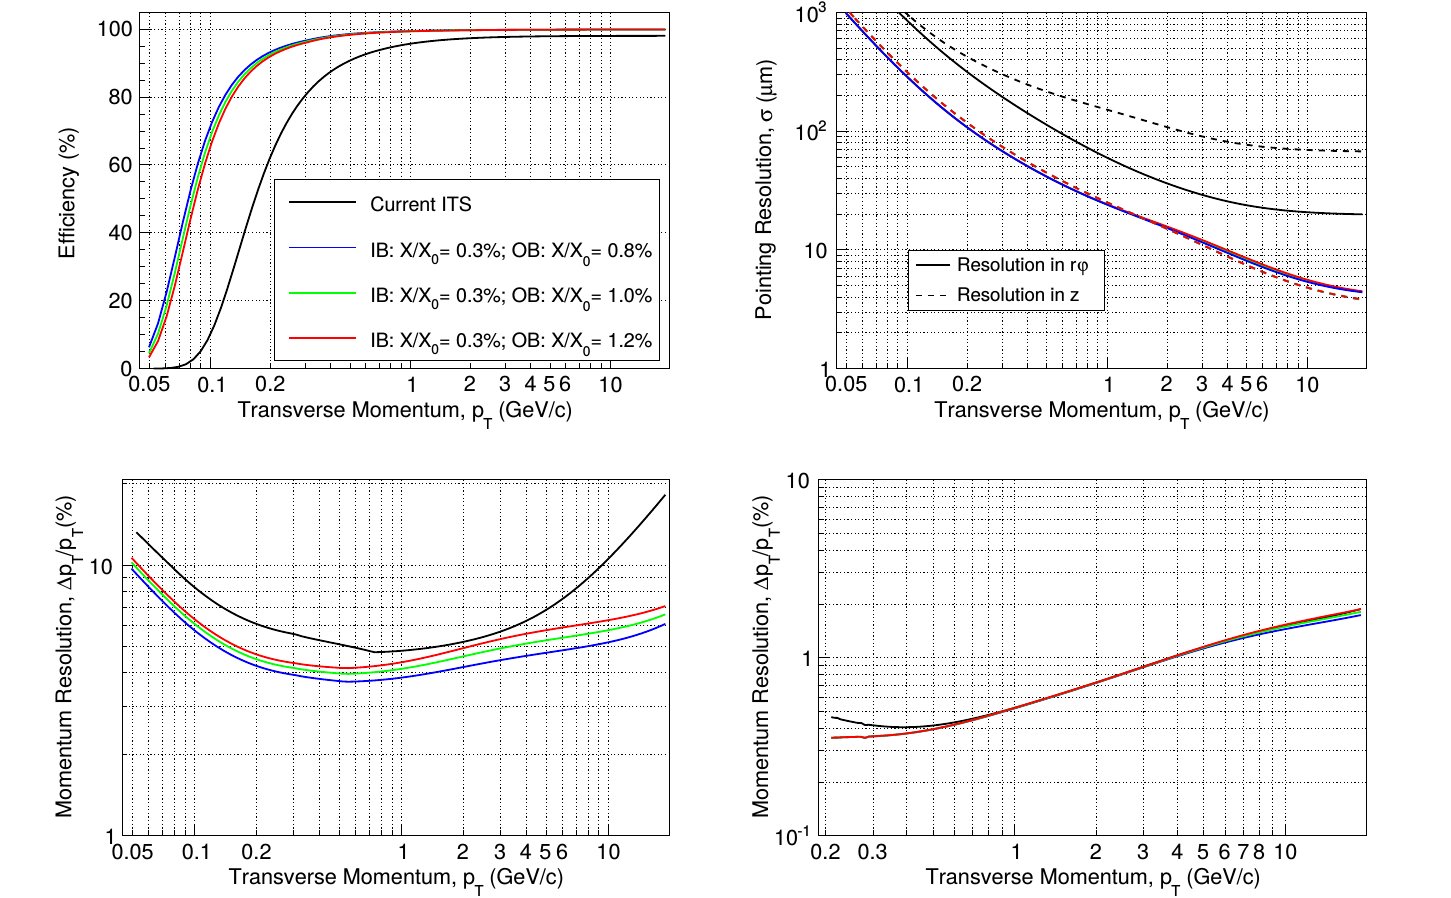
\includegraphics[scale=0.4]{figures/upperf.png}
  \caption{Stand-alone tracking efficiency (top-left panel) and pointing resolution (top-right panel) for charged pions of the current ITS and different material budget options for the ITSU. Transverse momentum resolution for charged pions for the current ITS and of the ITSU in stand-alone (bottom-left panel) and ITS+TPC (bottom-right panel) \cite{uptdr}.}
  \label{fig:upperf}
\end{figure}
%
In Figure \ref{fig:upperf} the results of the simulation for other important parameters of the upgraded detector are reported for different values of the material budget of the layers of the Outer Barrel. For the Inner Barrel a material budget of 0.3\% $X_0$ is always considered. The values are compared with the parameters of the current detector. Starting from the efficiency, there is not a significant difference between different values of material budget of the layers of the Outer Barrel, but in any case for each value of $\pt$ the efficiency is better. As far as the pointing resolution is concerned, its value will be better of about a factor of 5 in $r\varphi$ direction and of a factor of 20 in $z$ direction, due to the finest segmentation of the ITSU with respect to the current ITS.  The transverse momentum resolution in ITS stand-alone will improve with the upgrade and it is possible to notice its optimisation for lower material budget of the outer layers. In ITS+TPC mode, instead, there is not a big difference between different values of the material budget of the outer layers and, in general, an improvement is appreciable just for $\pt$ < 1 GeV/c.
\section{Physics Performances}
The heavy-flavour analysis is one of the fields that will benefit the most from the upgrade of the ITS. This is due to the better resolution of secondary vertices and impact parameters. In Figure \ref{fig:D0res} the case of the $D^0$ in the decay channel $D^0 \rightarrow K^-\pi^+$ is shown. In this figure the vertex resolutions for the current and the upgraded ITS, obtained via Monte Carlo simulations,  are reported. For the ITSU two kinds of simulations have been used: the \textit{full simulation} is a simulation completely based on the parameters of the upgraded detector, while the \textit{hybrid simulation} is based on existing Monte Carlo simulations for the current detector setup, scaled by the ratio between the resolution of the upgraded and the current detector as a function of $\pt$. It is possible to appreciate how the resolution of the secondary vertices improves of a factor of 3 in $x$ direction (and also in $y$ direction) and of a factor of 6 in $z$ direction. The consequence of this improvement in the vertex reconstruction is a better impact parameter resolution, which will improve of a factor of 3 with respect to the current ITS. Finally, from the previous consideration, the signal to noise ratio for the $D^0$ in the $D^0 \rightarrow K^-\pi^+$ decay channel can be estimated: for $\pt$ < 8 GeV/c there is an improvement of about a factor of 5, while for $\pt$ > 8 GeV/c it is better of a factor of 10 with respect to the current configuration. The two last comparisons can be seen in Figure \ref{fig:d0stuff}. This is just an example of how the measurement of heavy-flavours will benefit from the upgrade, but in general this improvement can be seen in all the D-meson measurements and also in B-meson measurements, since most of B-meson decay channels include a $D^0$ particle. Also the measurements of the heavy-flavour baryons will take advantage of the improved resolution and of the higher acquisition rate, i.e. higher statistics, that characterize the upgraded ITS.\\
The measurement of low-mass dielectrons in Pb-Pb collisions, not possible with the current detector, will be even more challenging, since there is the necessity to detect dileptons with an invariant mass down to $M_{ee} \approx 150$ MeV/$c^2$, that means to detect electrons with transverse momentum down to 100 - 200 MeV/c. This measurement is extremely difficult due to the huge combinatorial background, constituted of the electrons coming from $\pi^0$ Dalitz decays and from photon conversions. Thanks to the reduced material budget and the consequently enhanced low-$\pt$ tracking capability of the ITSU, it will be possible to track electrons down to $\pt \gtrsim $ 50 MeV/c, improving the reconstruction efficiency for those phenomena that form the combinatorial background.
%
\begin{figure}
  \centering
  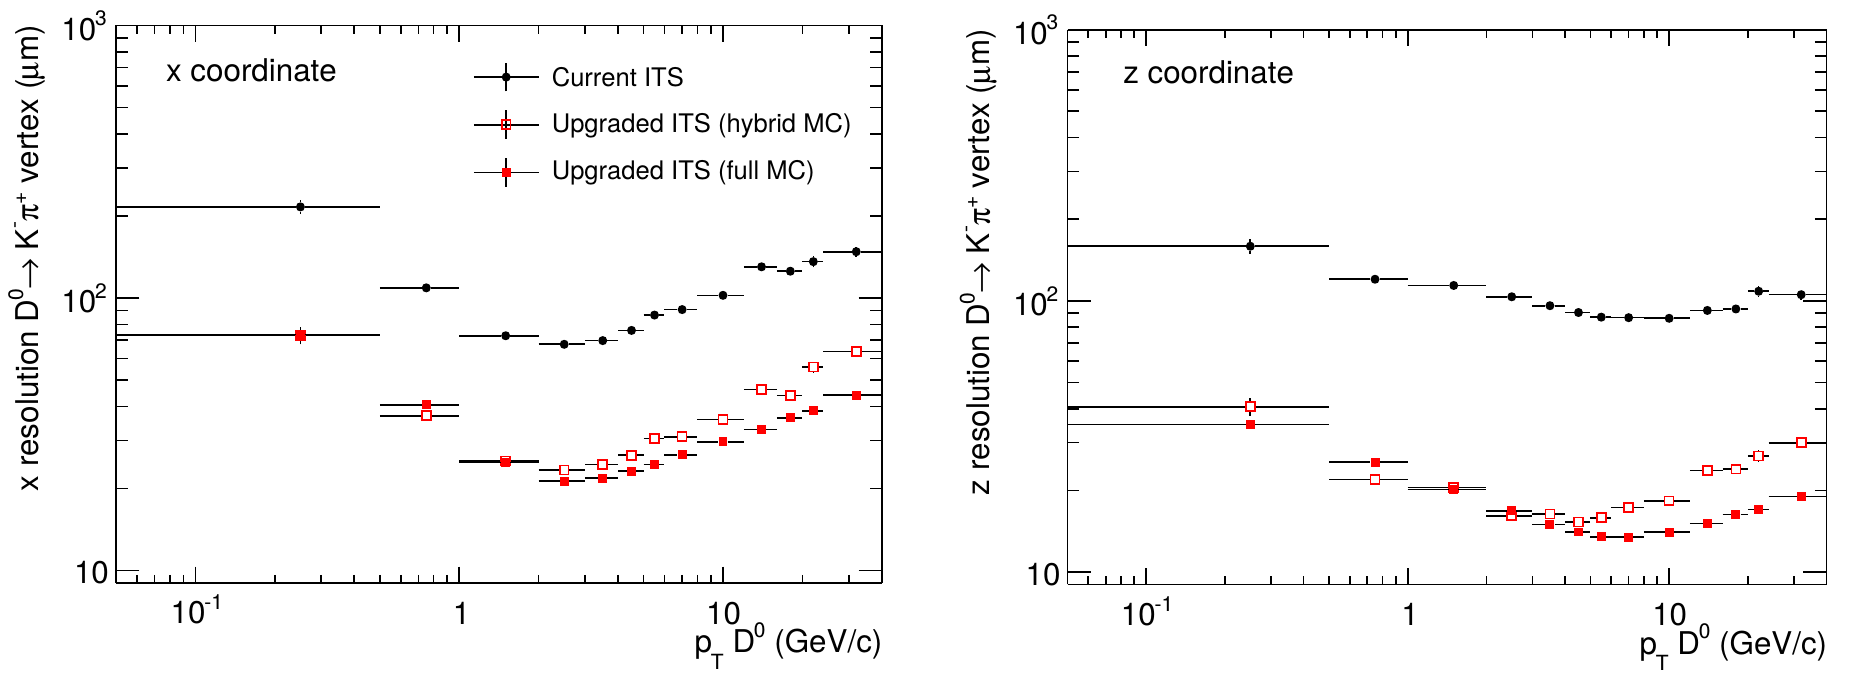
\includegraphics[scale=0.3]{figures/D0res.png}
  \caption{$D^0 \rightarrow K^-\pi^+$ secondary vertex position resolution for current and upgraded ITS in $x$ (left panel) and $z$ (right panel) \cite{uptdr}.}
  \label{fig:D0res}
  \vspace{1 cm}
  \centering
  {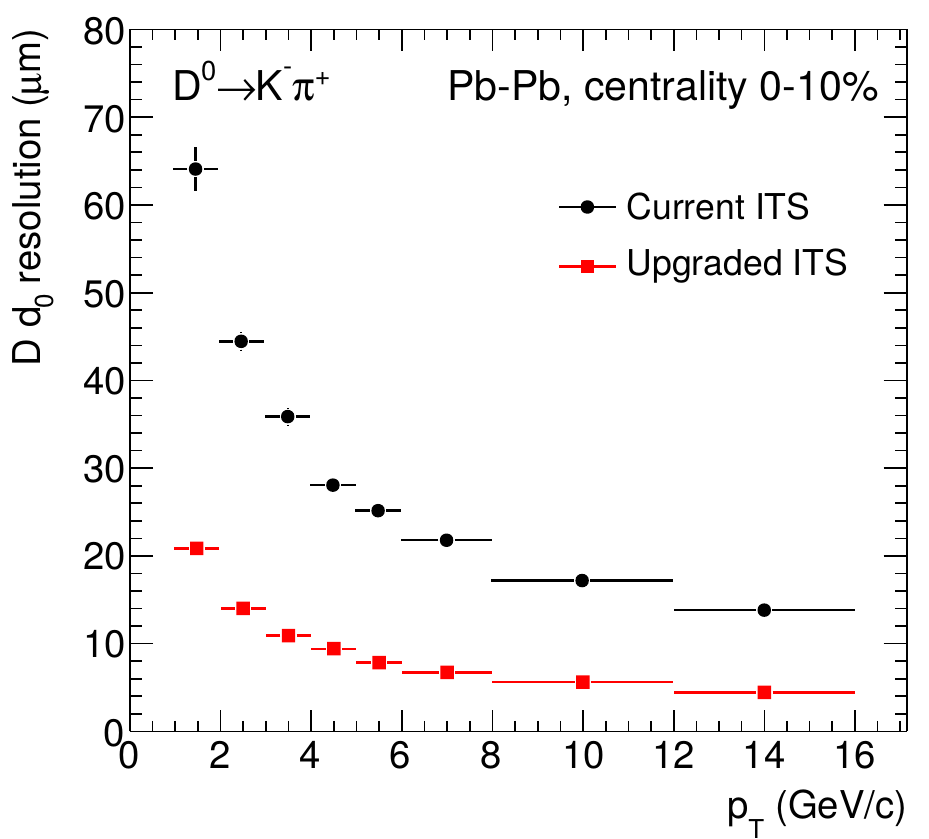
\includegraphics[scale=0.32]{figures/D0impres.png}}\quad
  {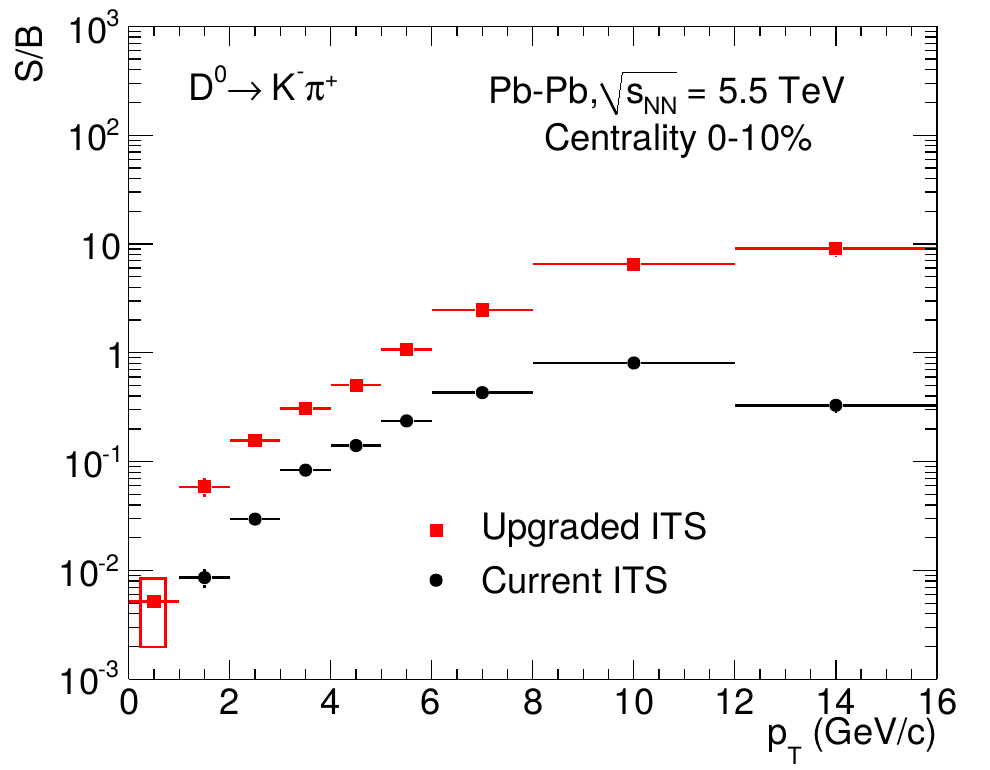
\includegraphics[scale=0.32]{figures/SoverB.png}}
  \caption{$D^0$ impact parameter resolution (upper panel) and $D^0$ signal-to noise ratio (lower panel) \cite{uptdr}.}
  \label{fig:d0stuff}
\end{figure}
\section{Online-Offline Computing System: O$^2$}
Mainly for the higher collision rate foreseen for Run3, but also for the increased number of readout channels, the data rate of the experiment will considerably increase after the upgrade, passing from the present value of about 25 GB/s to more than 1 TB/s. Almost the totality of this figure comes from the TPC, while the ITSU alone will provide 40 GB/s, that alone is more than the rate of all the detectors in the present configuration \cite{o2}. In order to deal with the new data rate, the DAQ, the HLT and the offline system will be replaced by a new Online-Offline integrated framework ($O^2$). The O$^2$ system will reduce the data volume online, in parallel with the data collection, without rejecting any event as with the trigger systems. In particular, the O$^2$ will perform a partial calibration and reconstruction online, substituting the original raw data with compressed data. The result is the production of \textit{Compressed Time Frames} (CTF), containing the processed data from all the active detectors for a period of time $\approx$ 20 ms. In particular, for the TPC and the ITS, the data are directly saved in cluster format. In addition, for the TPC, clusters not belonging to tracks or identified as background are rejected, allowing to compress the information to the maximum. From here on, CTFs are immutable and can be stored. Since this first reconstruction will be performed synchronously with the data acquisition, the O$^2$ facility will be equipped with hardware accelerators, such as \textit{Graphic Processing Units} (GPU) and \textit{Field Programmable Gate Arrays} (FPGA), to ensure sufficiently fast processing. Indeed, the first reconstruction can be performed with a high degree of parallelism because of the local and independent nature of the data. The following steps of the reconstruction are performed asynchronously, starting from the CTFs. Here an important role is played by the \textit{Grid}, the distributed computing system that connects the facilities of different institutes participating in the experiment \cite{tdrold}. A computing centre of the Grid is called \textit{Tier}: Tier-0 is the computing centre of CERN, Tier-1s are large regional centres and Tier-2s are small centres clustered around Tier-1s. For the data acquisition of Pb-Pb events, the O$^2$ facility will not be sufficient to process all the CTFs while performing the synchronous reconstruction. Indeed, only 2/3 of the asynchronous processes of reconstruction and calibration will be processed by the O$^2$ facility and the remaining 1/3 will be processed by Tier-0 and Tier-1s. The result of the second level asynchronous reconstruction is the production of \textit{Analysis Object Data} (AOD), which contain the final track parameters in a given vertex and for a given event. AOD are then analysed in dedicated \textit{High Performance Computing} (HPC) sites, called \textit{Analysis Facilities} (AF). AFs are capable of locally processing large data volumes: almost 5 PB in twelve hours.
\chapter{Cluster Shape Encoding}
In this chapter my work will be discussed. First there will be a description of the data format, the cluster of pixels, analysing its properties and the reason behind the encoding. Then, a detailed description of the methods implemented will follow. Finally, the test of such methods will be reported.
\section{Cluster of Pixels}
\label{sec:cluster}
As said in the last chapter, the sensors of ITS-Upgrade are characterized by a binary readout and therefore only the information whether or not a particle was crossing the pixel is read out. Pixels in which the collected charge coming from the ionization exceeds a defined threshold are called \textit{fired pixels}. When a charged particle passes through a sensor, it loses energy in a region whose dimension depends on the parameters of the particle itself, such as its energy and the impact angle. Therefore normally it fires a set of adjacent pixels.\\
%
\begin{figure}
  \centering
  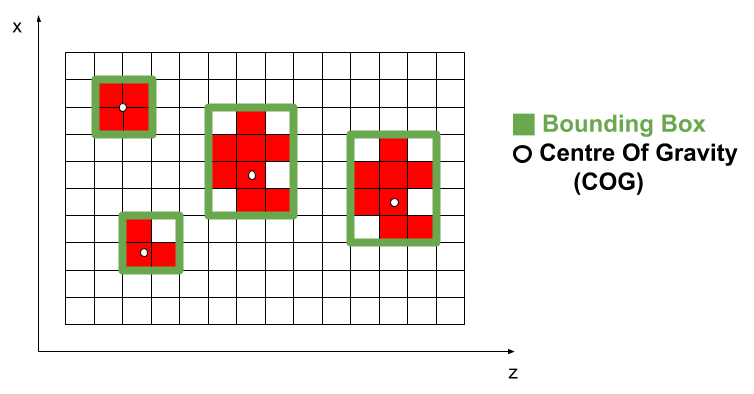
\includegraphics[scale=0.6]{figures/cluster.png}
  \caption{Example of different clusters on the same sensor. All the clusters have different positions, but two of them have the same shape.}
  \label{fig:clusters}
\end{figure}
%
A set of adjacent fired pixels forms a \textit{cluster}. Clusters are the data element of the ITS and are used for the reconstruction of the trajectories of the charged particles from which they have been generated. An example of clusters can be seen in Figure \ref{fig:clusters}. Each cluster in its raw format contains different kinds of information, which depend only on geometrical aspects. Each cluster has a particular shape, a specific pattern of fired pixels, which along my work is called \textit{topology}. As it can be seen in Figure \ref{fig:clusters}, different clusters can have the same topology.\\
Some characteristics are shared by clusters with the same topology. For example, the dimensions of the \textit{bounding box}, which is the smallest rectangle that can entirely contain the cluster, are clearly the same for all the clusters with the same shape. A second common piece of information is the position of the \textit{centre of gravity} (COG) of the topology within the bounding box, since this position is uniquely determined by the disposition of the fired pixels. The position of the COG is extremely important, since it is assumed to be the most probable impact position of the particle that generated the cluster. The uncertainty related to this quantity, which will be discussed later, is as well the same for all the clusters with the same topology.\\
The position of the cluster within the sensor is instead different from cluster to cluster. It is expressed as the coordinate of a reference pixel of the cluster within the matrix described by the pixels of the chip, in the form (\textit{row}, \textit{column}). The reference pixel of a cluster is defined as the pixel containing the COG of the cluster. This information is then converted into a physical length by a simple product of the coordinates by the pitch of the pixel. Each sensor has its own local frame, where z is the beam direction, x is orthogonal to z and lies on the surface of the sensor, y is orthogonal to the x-z plane, forming a right-handed Cartesian system. The passage from the local to the global frame is then performed during the reconstruction of the tracks, using matrices implemented in AliRoot.\\
In the next section the storage of the cluster data will be described, explaining the reasons behind this work.
\section{Data Compression}
The data size is an extremely important factor to hold in consideration during the design of a detector. The ALICE experiment, for example, has been designed for the study of heavy-ion collisions, with the necessity to identify all the particles produced in such collisions and to reconstruct their trajectories, and consequently a huge data volume is generated. As mentioned in section \ref{datavol}, after the trigger selection the data rate of all the detectors can reach 25 GB/s, while the physic content of many events could be small, with a DAQ archiving rate of about 1 GB/s. It is therefore clear that online processing is necessary to compress data avoiding the loss of physic content. The data rate will increase significantly after the upgrade, principally because of the higher collision rate. In particular, the data rate of all the detectors is estimated to be $\sim$ 1 TB/s \cite{o2}, where almost 1 TB/s is given by the TPC. For the ITS the data rate will increase both because of the higher collision rate and because of the higher number of readout channels ($\sim 10^{10}$). It is expected to be $\sim$ 40 GB/s, more than the current data rate of the whole ALICE apparatus. The data reduction starts immediately after the cluster-funding process and the information is compressed using Huffman coding, which will be shortly described in the next section. With Huffman compression it is possible to reduce the data size of a factor that depends on the the noise occupancy: in worst case scenario, with many noisy pixels, data size is reduced to  $\sim$ 26 GB/s, while in case of low noise it is reduced to $\sim$ 4.3 GB/s \cite{o2}.
\subsection{Huffman Coding}
\label{sec:huff}
Huffman coding is one of the most used lossless data compression algorithms, based on the relative frequency of the elements constituting a file. Huffman maps an element (for example a character in a text file) into a a bit sequence of variable length according to its frequency: the most frequent element is mapped into the shortest string. The result is a Huffman table, of which an example is given in Table\ref{tab:huff}. It is the Huffman table corresponding to the sentence ``\textit{Trentatrè trentini entrarono in Trento, tutti trentatrè trotterellando.}'': the most frequent character (t) is mapped into a two-bit sequence, while the least common ones are mapped in the longest bit strings. In this way it is possible to contain the information of the sentence in a shorter bit string. This example is trivial, but it allows to understand the utility of Huffman compression when applied to big files. Indeed, the most frequent character is encoded as the shortest bit string, therefore every time this character appears it is substituted by the corresponding Huffman code: the shortest string appears the highest number of times, allowing to save much storage space. Moreover, the less the frequency distribution of the elements is uniform, the more storage space is saved, since the most common character, hence the shortest bit string, appears much more often than the less common ones. This saving is obtained at the cost of creating a Huffman table and consulting it during the compression and the decompression processes, operations which are time consuming. For this reason, if the compression/decompression time is an important factor, it is necessary to pay attention to the number of entries in the table, since the former is proportional to the latter \cite{huffman}.
%
\begin{table}
\centering
 \begin{tabular}{|c|c|c|}
  \hline
  Character & Frequency & Huffman code\\
  \hline
  t & 15 & 01 \\
  r & 10 & 110 \\
  n & 9 & 101 \\
  e & 7 & 000 \\
  \_ & 7 & 001\\
  o & 5 & 1001 \\
  i & 4 & 11111 \\
  a & 3 & 11110 \\
  è & 2 & 10000 \\
  l & 2 & 10001 \\
  T & 2 & 111011 \\
  u & 1 & 111010 \\
  , & 1 & 111001 \\
  . & 1 & 111000 \\
  \hline
 \end{tabular}
 \caption{Huffman table related to the sentence ``\textit{Trentatrè trentini entrarono in Trento, tutti trentatrè trotterellando.}''.}
 \label{tab:huff}
\end{table}
%
\section{Cluster Data Encoding}
Every cluster is identified by its position and its topology. In section \ref{sec:cluster} it was said that the position of the cluster can be expressed as the coordinates of the reference pixel of the cluster within the sensor. This information must be combined with an identifier of the chip, whose position in the experiment frame is known. It is possible to store the position of the reference pixel not as its absolute raw number, but as the difference between its row number and that of the previous stored pixel. Studying the frequency distributions of these deltas, it can be seen that it is not uniform and consequently it is possible to benefit from this non uniformity using Huffman coding. Similarly, the identifiers of the chips can be stored as the difference between the identifier of the chip which is being analysed and the previous one. Its distribution is not uniform as well and this element can be compressed using Huffman too. Both this distributions are strongly dependent on the occupancy in the detector. For this reason it is possible to use different Huffman tables according to the multiplicity. In particular the multiplicity can be binned and for each multiplicity bin a Huffman table is defined. This information, together with the topology, defines the cluster data:
\begin{displaymath}
\begin{split}
  \mathrm{MultID[\textcolor{red}{\Delta ChipID_1}(\textcolor{Cerulean}{Col}, \textcolor{LimeGreen}{\Delta Row}, \textcolor{Plum}{Patt})_1 \  ... \ (\textcolor{Cerulean}{Col}, \textcolor{LimeGreen}{\Delta Row}, \textcolor{Plum}{Patt})_n \textcolor{SkyBlue}{\Delta EndChip}] }\\
 \mathrm{[\textcolor{red}{\Delta ChipID_2}(\textcolor{Cerulean}{Col}, \textcolor{LimeGreen}{\Delta Row}, \textcolor{Plum}{Patt})_1 \  ... \ (\textcolor{Cerulean}{Col}, \textcolor{LimeGreen}{\Delta Row}, \textcolor{Plum}{Patt})_n \textcolor{SkyBlue}{\Delta EndChip}]\ ...}
 \end{split}
\end{displaymath}
\textit{MultID} is the multiplicity bin, used to pick up the appropriate Huffman table to encode/decode the information about the row number and the identifier of the chip; \textit{$\Delta$ChipID} is the difference between the identifier of the cluster being analysed and the previous one; \textit{Col} is the column number of the reference pixel; \textit{$\Delta$Row} is the difference between the row number of the reference pixel of the current cluster and the previous one. \textit{EndChip} is a special identifier that flags the end of the chip. \textit{Patt} is instead the information related to the topology, which will be discussed in the next section.
\section{Cluster Topology Encoding}
The cluster topology, in its raw format, consists of a sequence of bits whose length depends on the number of pixels within the bounding box: a fired pixel is represented by a 1, while an off one by a 0. Such a string can become very long for large clusters, therefore storing the information about the cluster topology as the complete bit-mask would require the usage of much storage space.
%
\begin{figure}
  \centering
  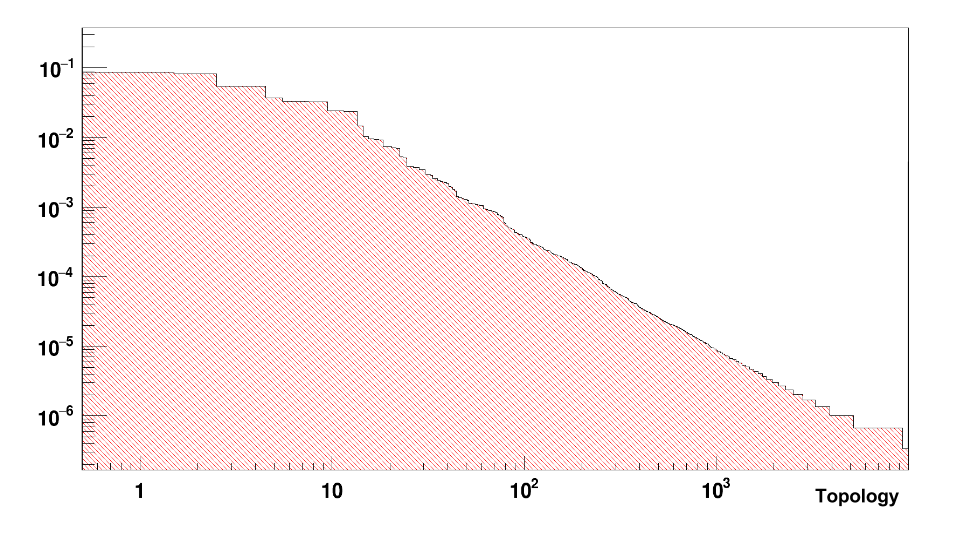
\includegraphics[scale=0.4]{figures/topdistro.png}
  \caption{Frequency distribution of the topologies obtained through a Monte Carlo simulation of 20 Pb-Pb events.}
  \label{fig:topdistro}
\end{figure}
%
This issue can be solved creating a dictionary containing all the topologies. In this way it is possible to store a reference to an entry of the dictionary instead of the complete bit-mask. Since a reference is an integer, its length is fixed. In Figure \ref{fig:topdistro} a frequency distribution of the topologies, obtained simulating 20 minimum-bias Pb-Pb events, is reported. This distribution is highly non uniform and consequently the compression via Huffman would be extremely convenient in terms of storage space. However, due to the high number of different elements, the processes of compression and decompression become inefficient. Therefore, there is the necessity to reduce the number of entries in the dictionary and this can be done grouping rare topologies, whose frequency is under a defined threshold, under a common reference.\\
In the next sections the steps to the construction of the dictionary of the topologies will be described and a detailed description about the method of grouping will be given.
\section{Software Development}
The objective of this work is the implementation of some software for the construction of the dictionary and for the realisation of the related mechanisms of matching between the cluster topology the corresponding entry in the dictionary. In particular this software will be used online, during the data acquisition in Run3. It must not be developed to work in AliRoot or ROOT environment: the two data analysis frameworks contain many features that are not necessary during the data acquisition and therefore the machines used for online operations have nor AliRoot and ROOT installed. For this reason several C++ classes, which can be used on every machine with a C++ compiler installed, have been implemented:
\begin{itemize}
 \item \textbf{MinimTopology} is a support class which contains the whole information necessary to characterize a topology;
 \item \textbf{Dictionary} is the proper dictionary, containing the information about all the common topologies and the groups of rare topologies;
 \item \textbf{BuildDictionary} is the class dedicated to the construction of the dictionary starting from the data;
 \item \textbf{LookUp} is used to match online the topology of clusters with the corresponding entry in the dictionary;
 \item \textbf{FastSimulation} can simulate a population of topologies with a frequency distribution determined by the dictionary. 
\end{itemize}
\section{Uniqueness of the Keys in the Dictionary: Hash Functions}
The dictionary must fulfill few requirements. First of all, each entry in the dictionary must be uniquely identified by a key. The key must have specific characteristics: it must have a defined length, which must be the same for each entry of the dictionary, and it must be comparable with the other keys, in order to be sortable. Typically in a database the key is an integer, since such a type has the needed characteristics. Unfortunately the topology is a bit string whose length is determined by the size of the bounding box and it cannot be used as a key. It is necessary to convert the topology as a string of variable length into a string of defined length. This operation is performed using a \textit{hash function}, which is a function that maps data of arbitrary size into data of fixed size. In particular in this work a C++ implementation of the function MurmurHash2 is used. The name suggests its working principle, since it is the combination of the words multiply (Mu) and rotate (r): MurmurHash2 processes the input string four bytes at a time, performing bitwise and multiplication operations, and combines all the four-byte chunks to give as a result a four-byte sequence. The choice of MurmurHash2 was made considering its characteristics: it has a good uniformity of the output distribution and is fast if compared with other algorithms \cite{hash}. Indeed, the hash function must be as fast as possible, since it must be used online. The uniformity of the output instead is related to the non injectivity of the hush function: while the input of the hash function can be any string of bits, the output must be a positive integer (four-byte sequence) and therefore can be each integer in the range [0, 2$^{32}$ - 1]. If the distribution of the outputs is uniform, then its more likely that two different input strings are mapped into two different integers. Unfortunately, even if the MurmurHash2 function has a good uniformity, it is not injective: in very rare cases (< 1/1000) two different strings are mapped into the same hashcode. All the classes must be solved to use the dictionary: this operation is done in the class \textit{MinimTopology}, which will be described in the next section.
%
\begin{figure}
  \centering
  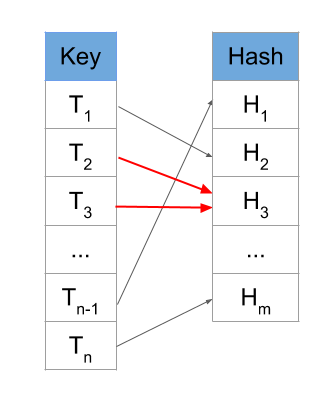
\includegraphics[scale=0.5]{figures/clash.png}
  \caption{Example of clash: MurmurHash2 maps two topologies (T$_2$ and T$_3$) into the same hashcode (H$_3$).}
  \label{fig:clash}
\end{figure}
%
\section{Class MinimTopology}
The class MinimTopology is the basis of this work since it is used by all the other classes. This class contains the information necessary to characterize a topology: the pattern, in string format, and the corresponding hashcode, generated from the first with a method that will be described soon. Starting from the pattern, the only sequence of bits is not enough to identify uniquely. For example, the sequence 1111 could represent four fired pixels in a raw, or four fire pixels in a column, or a square of four pixels, all fired. Beside this information also the dimensions of the bounding box are needed. In this way it is possible to correctly interpret the sequence of pixels that constitutes the pattern. An example of pattern encoding within the class MinimTopology is given in Figure \ref{fig:pattern}. This topology has three rows and three columns, corresponding to a sequence of nine pixels. The pattern is encoded in a string where the first two bytes are respectively the number of rows and the number of columns. The remaining bytes of the string are used to encode the proper pattern, i.e. the sequence of pixels that constitutes the topology itself. In the example the pattern consists of nine pixels, therefore two bytes are necessary, since a byte is made of 8 bits. A 1 is associated to each fired pixel, a 0 to each off one. From this string a four-byte hashcode is generated using MurmurHash2, but at this stage it is possible that two different patterns are mapped into the same 4-byte sequence. There is therefore the necessity to solve the clashes. One method could be to mark with a flag the entries of the dictionary for which there is a clash and then proceed with the direct comparison between the patterns until the ambiguity is erased. However this method require additional operations: first it is necessary to check whether the hashcode is marked with a clash-flag (even if there are not collisions) and then to resolve the ambiguities through a direct comparison. In fact there is a method to avoid the useless operation of the flag check: it is possible to use a eight-byte hashcode, in which the first four bytes are the usual four-byte hashcode previously described and the last four bytes are the first four byte which constitutes the pattern (the bytes starting from the third one of the string). In this way when two eight-byte hashcodes are compared it is performed both a comparison of the hash generated with MurmurHash2 and of the first 32 pixels, so that in case two different topologies are mapped into the same four-byte sequence by the hash function the clash is solved at the same time of the four-byte hashcode comparison.
\begin{figure}
  \centering
  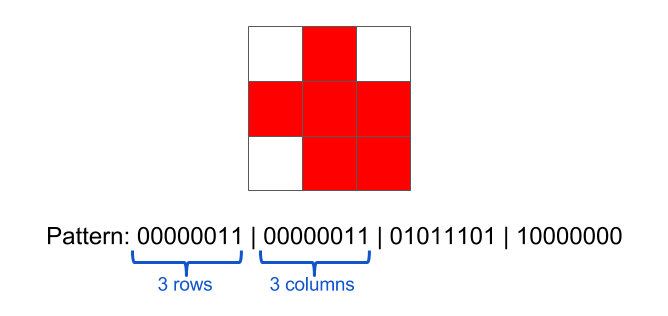
\includegraphics[scale=0.5]{figures/pattern.png}
  \caption{Example of pattern encoding: the first two bytes are respectively the number of rows and the number of columns; the remaining bytes are the pattern itself.}
  \label{fig:pattern}
\end{figure}
%
Summing up, the class MinimTopology has two data members:
\begin{enumerate}
 \item a string in which the pattern of pixels is stores;
 \item a eight-byte hashcode, generated from the pattern with the method just described, which uniquely identifies the topology.
\end{enumerate}
%
\section{Reduction of the Entries of the Dictionary: Grouping}
The second requirement for the dictionary concerns the number of entries. As said in section \ref{sec:huff}, the Huffman becomes inefficient when the number of different elements (in this case the number of topologies within the dictionary) is high. For this reason there is the necessity to limit the number of entries of the dictionary to at most O(10$^3$). This objective is achieved grouping rare topologies under a common reference, called \textit{GroupID}. The groups must be formed to gather rare topologies with similar characteristics, i.e. with similar errors related to the estimated impact position of the particle that generated the cluster. The grouping is necessary a lossy operation, since the information about the pattern of pixels, and therefore about the position of the impact point of the single rare topology, is lost in favour of average quantities. However this loss is bearable, since it concerns rare topologies and therefore it interests a very small fraction of the data.\\
The chosen grouping criterium concerns the dimensions of the bounding box: it is based on the assumption that topologies with similar dimensions have similar uncertainties related to the impact point position. As it will be seen later, for each topology the uncertainty on the impact point position is get from the distribution of the impact points themselves (or rather their first reconstruction) with respect to the COG position. In the case of groups of rare topologies this method is not applicable, since in different topologies the position of the COG within the bounding box can be extremely different and the distribution of the impact points (their first reconstruction) can be different too. Since it is not possible to rely on these distributions, the error is evaluated with the most pessimistic method: the position of the COG is assumed to be equally probable in the whole area of the bounding box. The error associated to the position of the COG is therefore that of a uniform distribution. In particular, a uniform distribution in the range of x(z) dimension of the bounding box:
\begin{equation}
 \sigma_x \; = \; \frac{N_{rows} \cdot d_x}{\sqrt{12}} \ \ \ \ \  \sigma_z \; = \; \frac{N_{columns} \cdot d_z}{\sqrt{12}}
\end{equation}
Considering a uniform distribution maybe the error is a bit overestimated, but it must be considered that this approximation involves rare topologies and hence a very small fraction of the data.\\
The grouping is based on a two-dimensional binning: a rare topology is assigned to a particular group according to its number of columns and rows. An example of grouping can be seen in Figure \ref{fig:gruppi}.

\begin{figure}
  \centering
  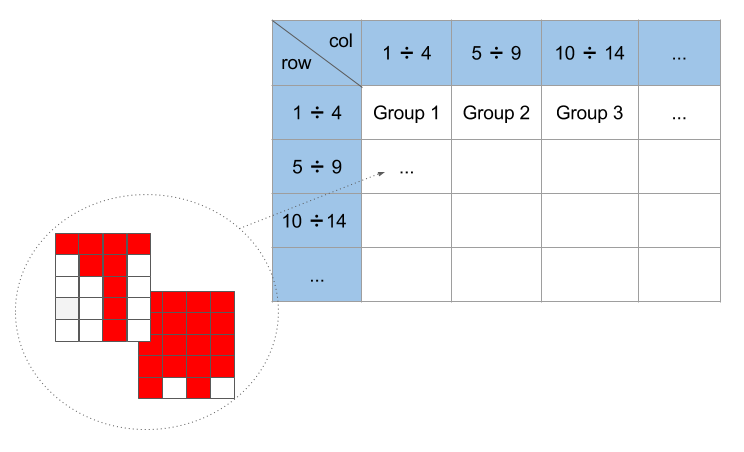
\includegraphics[scale=0.5]{figures/gruppi.png}
  \caption{Example of grouping: the two rare topologies have the same number of rows and columns and belong to the same group.}
  \label{fig:gruppi}
\end{figure}
%
\printbibliography


\end{document}          
